\documentclass[hyphens,aspectratio=169]{beamer}
\usepackage{tikz}
\usetikzlibrary{arrows.meta, positioning}
\usepackage{animate} % for \animategraphics
\usepackage{graphicx}
\usepackage[export]{adjustbox} 
\usepackage{amssymb}
\usepackage{amsmath}
\usepackage{mathtools}
\usepackage{textcomp}
 \usepackage[normalem]{ulem}
\usepackage{moresize}
\usepackage{framed}
\usepackage{minted}
\usepackage{relsize}
\usepackage{algorithm}
\usepackage{algpseudocode}
\graphicspath{{../}}
\usetheme{Berlin}
\usecolortheme[RGB={0,95,47}]{structure}
\beamertemplatenavigationsymbolsempty
\addtobeamertemplate{navigation symbols}{}{%
    \usebeamerfont{footline}%
    \usebeamercolor[fg]{footline}%
    \hspace{1em}%
    \insertframenumber/\inserttotalframenumber
}
\newcommand\blfootnote[1]{%
  \begingroup
  \renewcommand\thefootnote{}\footnote{#1}%
  \addtocounter{footnote}{-1}%
  \endgroup
}
\makeatletter
\AtBeginEnvironment{minted}{\dontdofcolorbox}
\def\dontdofcolorbox{\renewcommand\fcolorbox[4][]{##4}}
\setbeamertemplate{footline}{}            % removes the entire bottom bar
\makeatother
\title{Action This Day!}
\subtitle{The Mathematics and Machinations that Bested the German Enigma}
\author{Jonah Weinbaum}
\date{
July 28, 2025
}
\begin{document}

\frame{\titlepage}

\section{Action This Day}

% \begin{frame}[fragile]{D-Day}
% 	\begin{center}
% 		\begin{figure}
% 			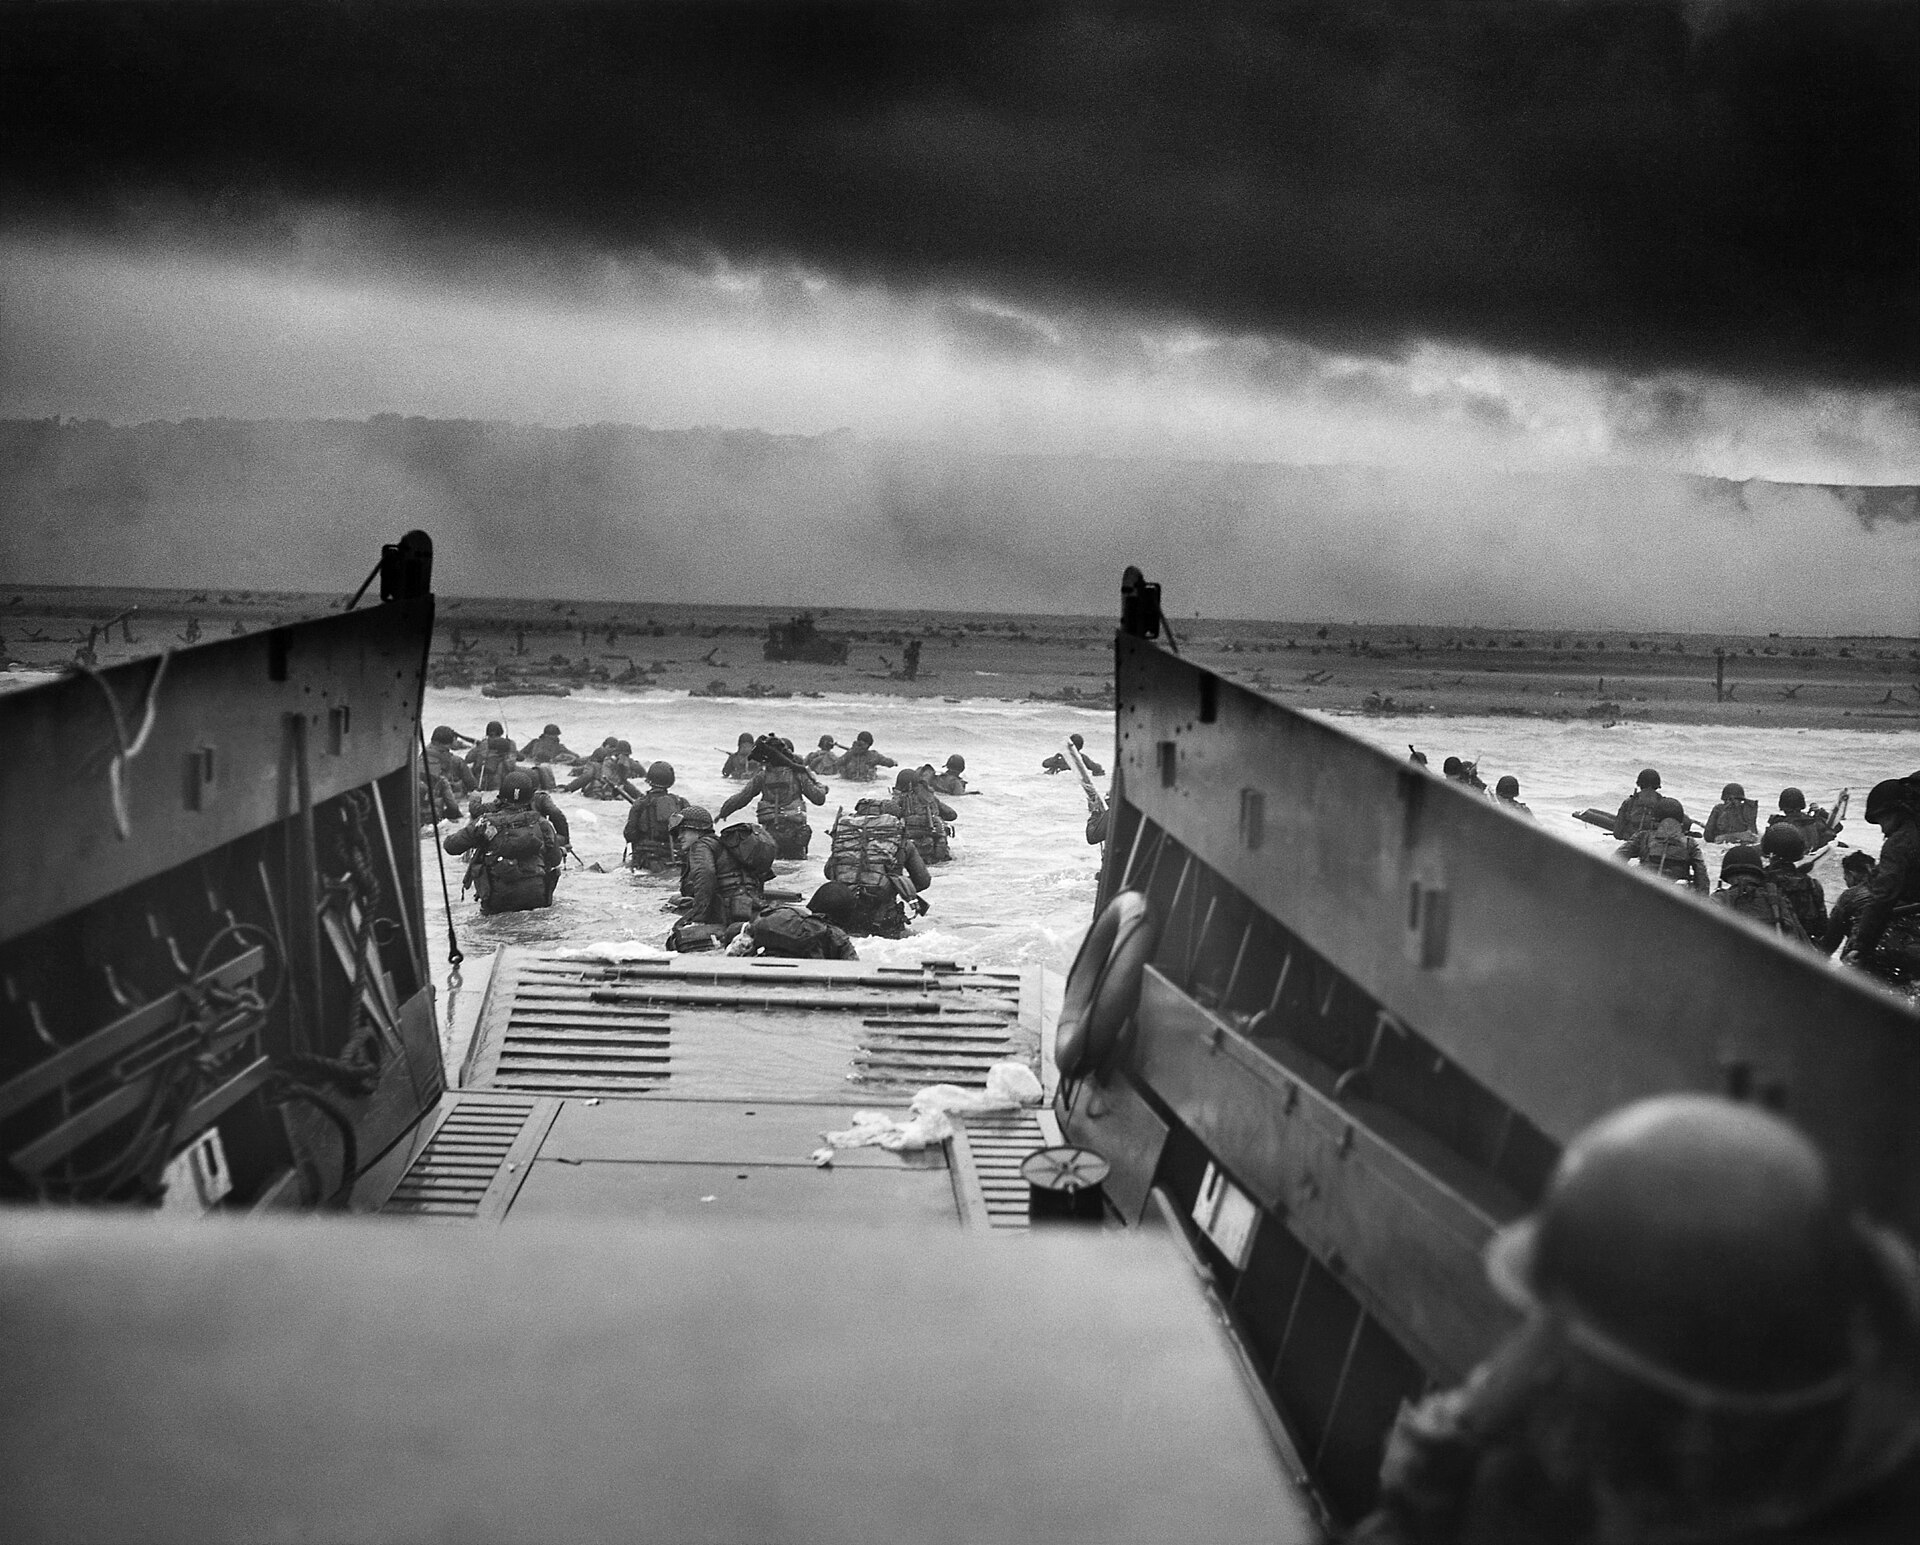
\includegraphics[scale=0.11]{paper/images/dday.jpg}
% 			\small
% 			\caption{\emph{Into the Jaws of Death} -- Robert F. Sargent -- June 6, 1944 (D-Day)}
% 		\end{figure}

% 	\end{center}
% \end{frame}

% \begin{frame}[fragile]{D-Day}
% 	\begin{center}
% 		\begin{figure}
% 			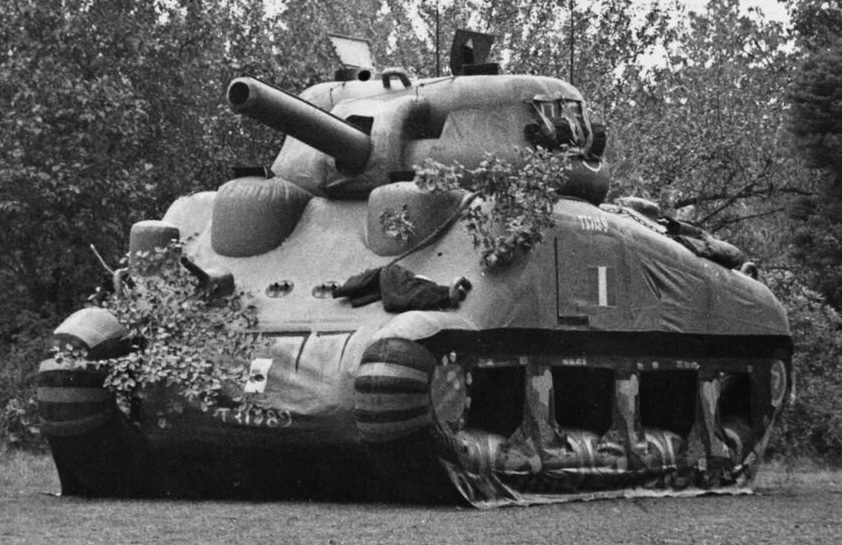
\includegraphics[scale=0.3]{paper/images/dummy_tank.jpg}
% 			\small
% 			\caption{Inflatable M4 Sherman Tank -- Operation Bodyguard}
% 		\end{figure}

% 	\end{center}
% \end{frame}

% \begin{frame}[fragile]{D-Day}
% 	Allied forces needed to time the invasion around
% 	\begin{itemize}
%         \setlength\itemsep{1em}
% 		\item Time of day
% 		      \pause
% 		\item Weather
% 		      \pause
% 		\item Tides
% 		      \pause
% 		\item Phase of the moon
% 	\end{itemize}

% \end{frame}

% \begin{frame}[fragile]{D-Day}
% 	The invasion was scheduled for June 5th,
% 	\pause
% 	then postponed to June 6th
% 	\pause
% 	\\\\Further postponement would move the plan a month.
% \end{frame}

% \begin{frame}[fragile]{D-Day}
% 	\begin{center}
% 		\begin{figure}
% 			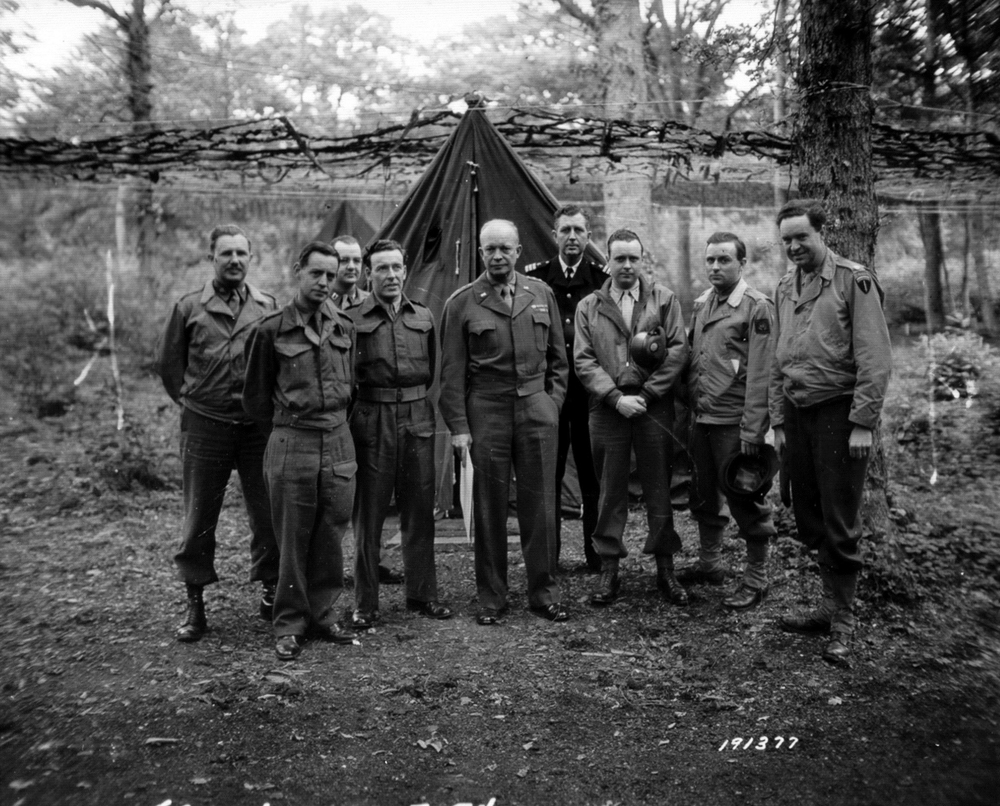
\includegraphics[scale=0.21]{paper/images/general_eisenhower.jpg}
% 			\small
% 			\caption{General Eisenhower's advance command post near Southwick House}
% 		\end{figure}

% 	\end{center}
% \end{frame}

% \begin{frame}[fragile]{D-Day}
% 	\begin{center}
% 			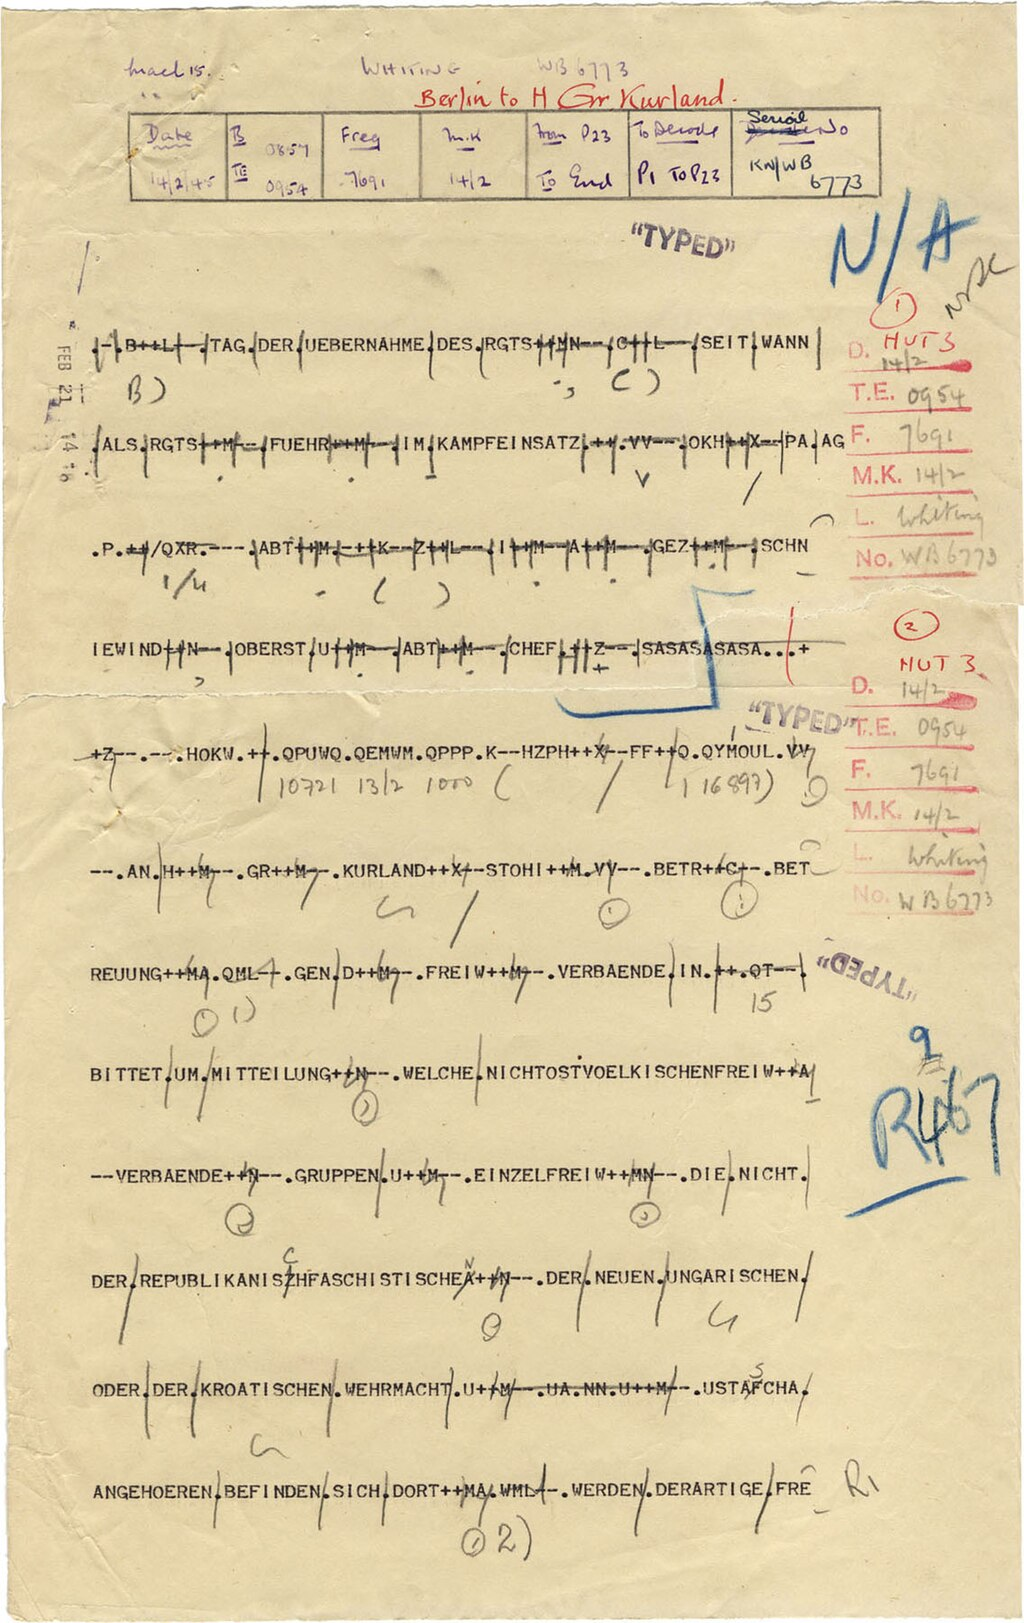
\includegraphics[scale=0.115]{paper/images/bletchley_decrypt.jpg}
% 	\end{center}
% \end{frame}

\begin{frame}[fragile]{Action This Day}
	\begin{center}
		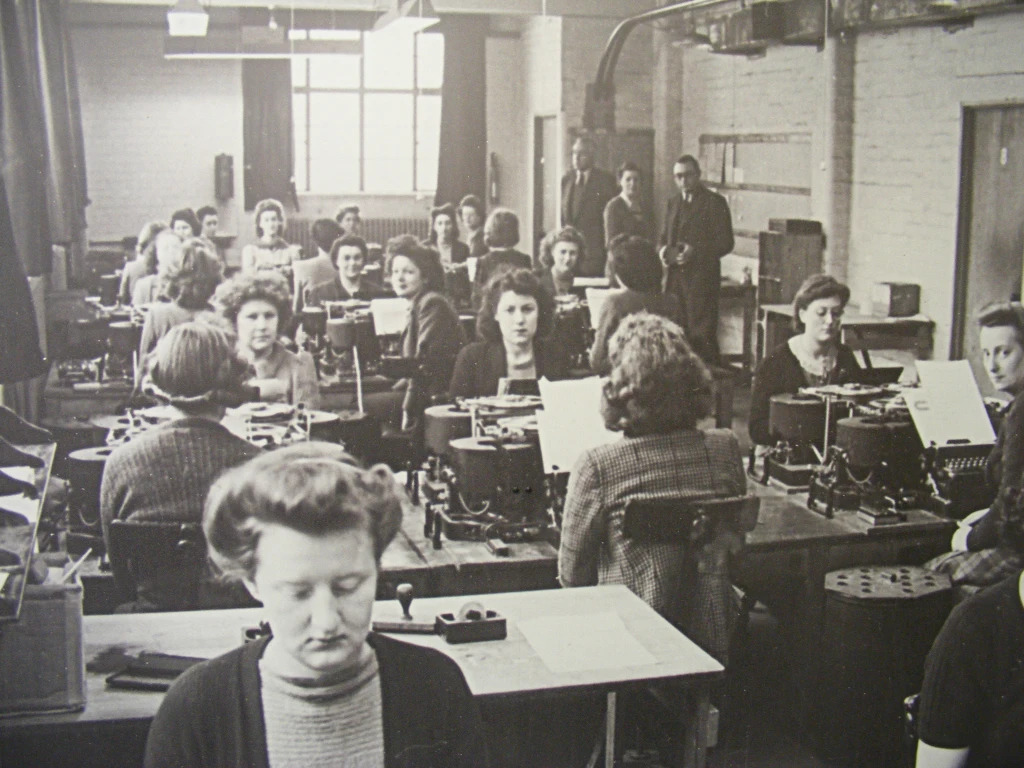
\includegraphics[scale=0.23]{paper/images/codebreakers.jpg}
	\end{center}
\end{frame}

\begin{frame}[fragile]{Action This Day}
	\begin{center}
		
\includegraphics[scale=0.3]{paper/images/action_this_day.jpg}
	\end{center}
\end{frame}

\begin{frame}[fragile]{Action This Day}
	\begin{center}
		\scalebox{0.9}{
			\begin{minipage}{0.48\textwidth}
				\centering
				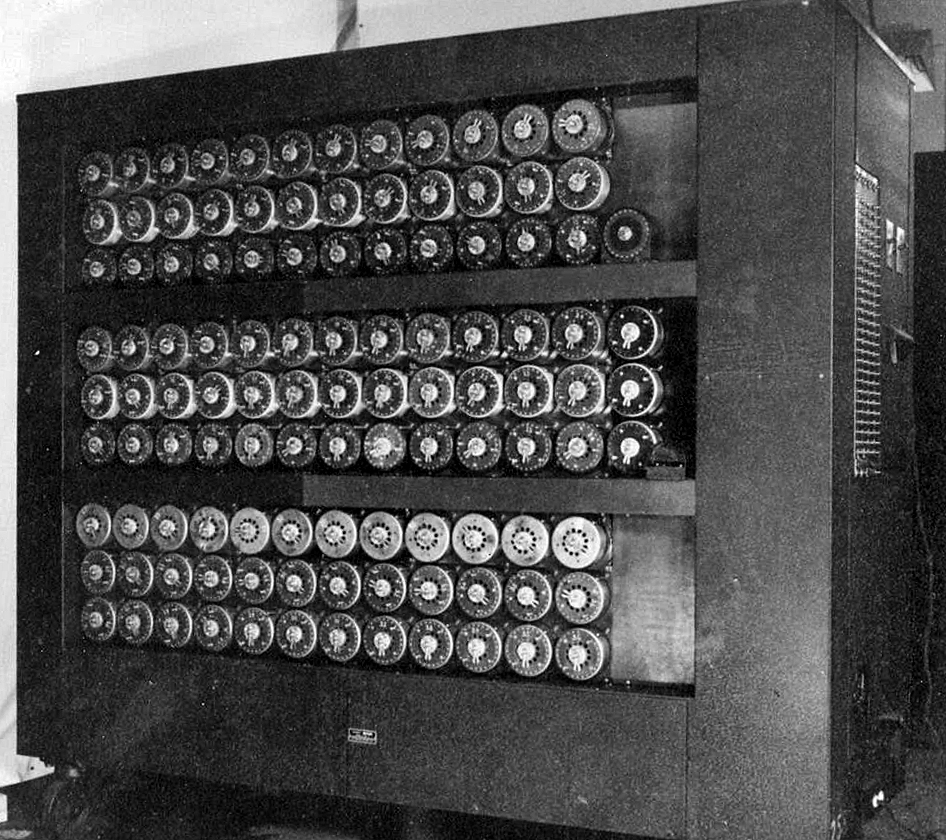
\includegraphics[width=\linewidth]{paper/images/bombe.jpg}
			\end{minipage}%
			\hfill
            
			\begin{minipage}{0.48\textwidth}
				\centering
				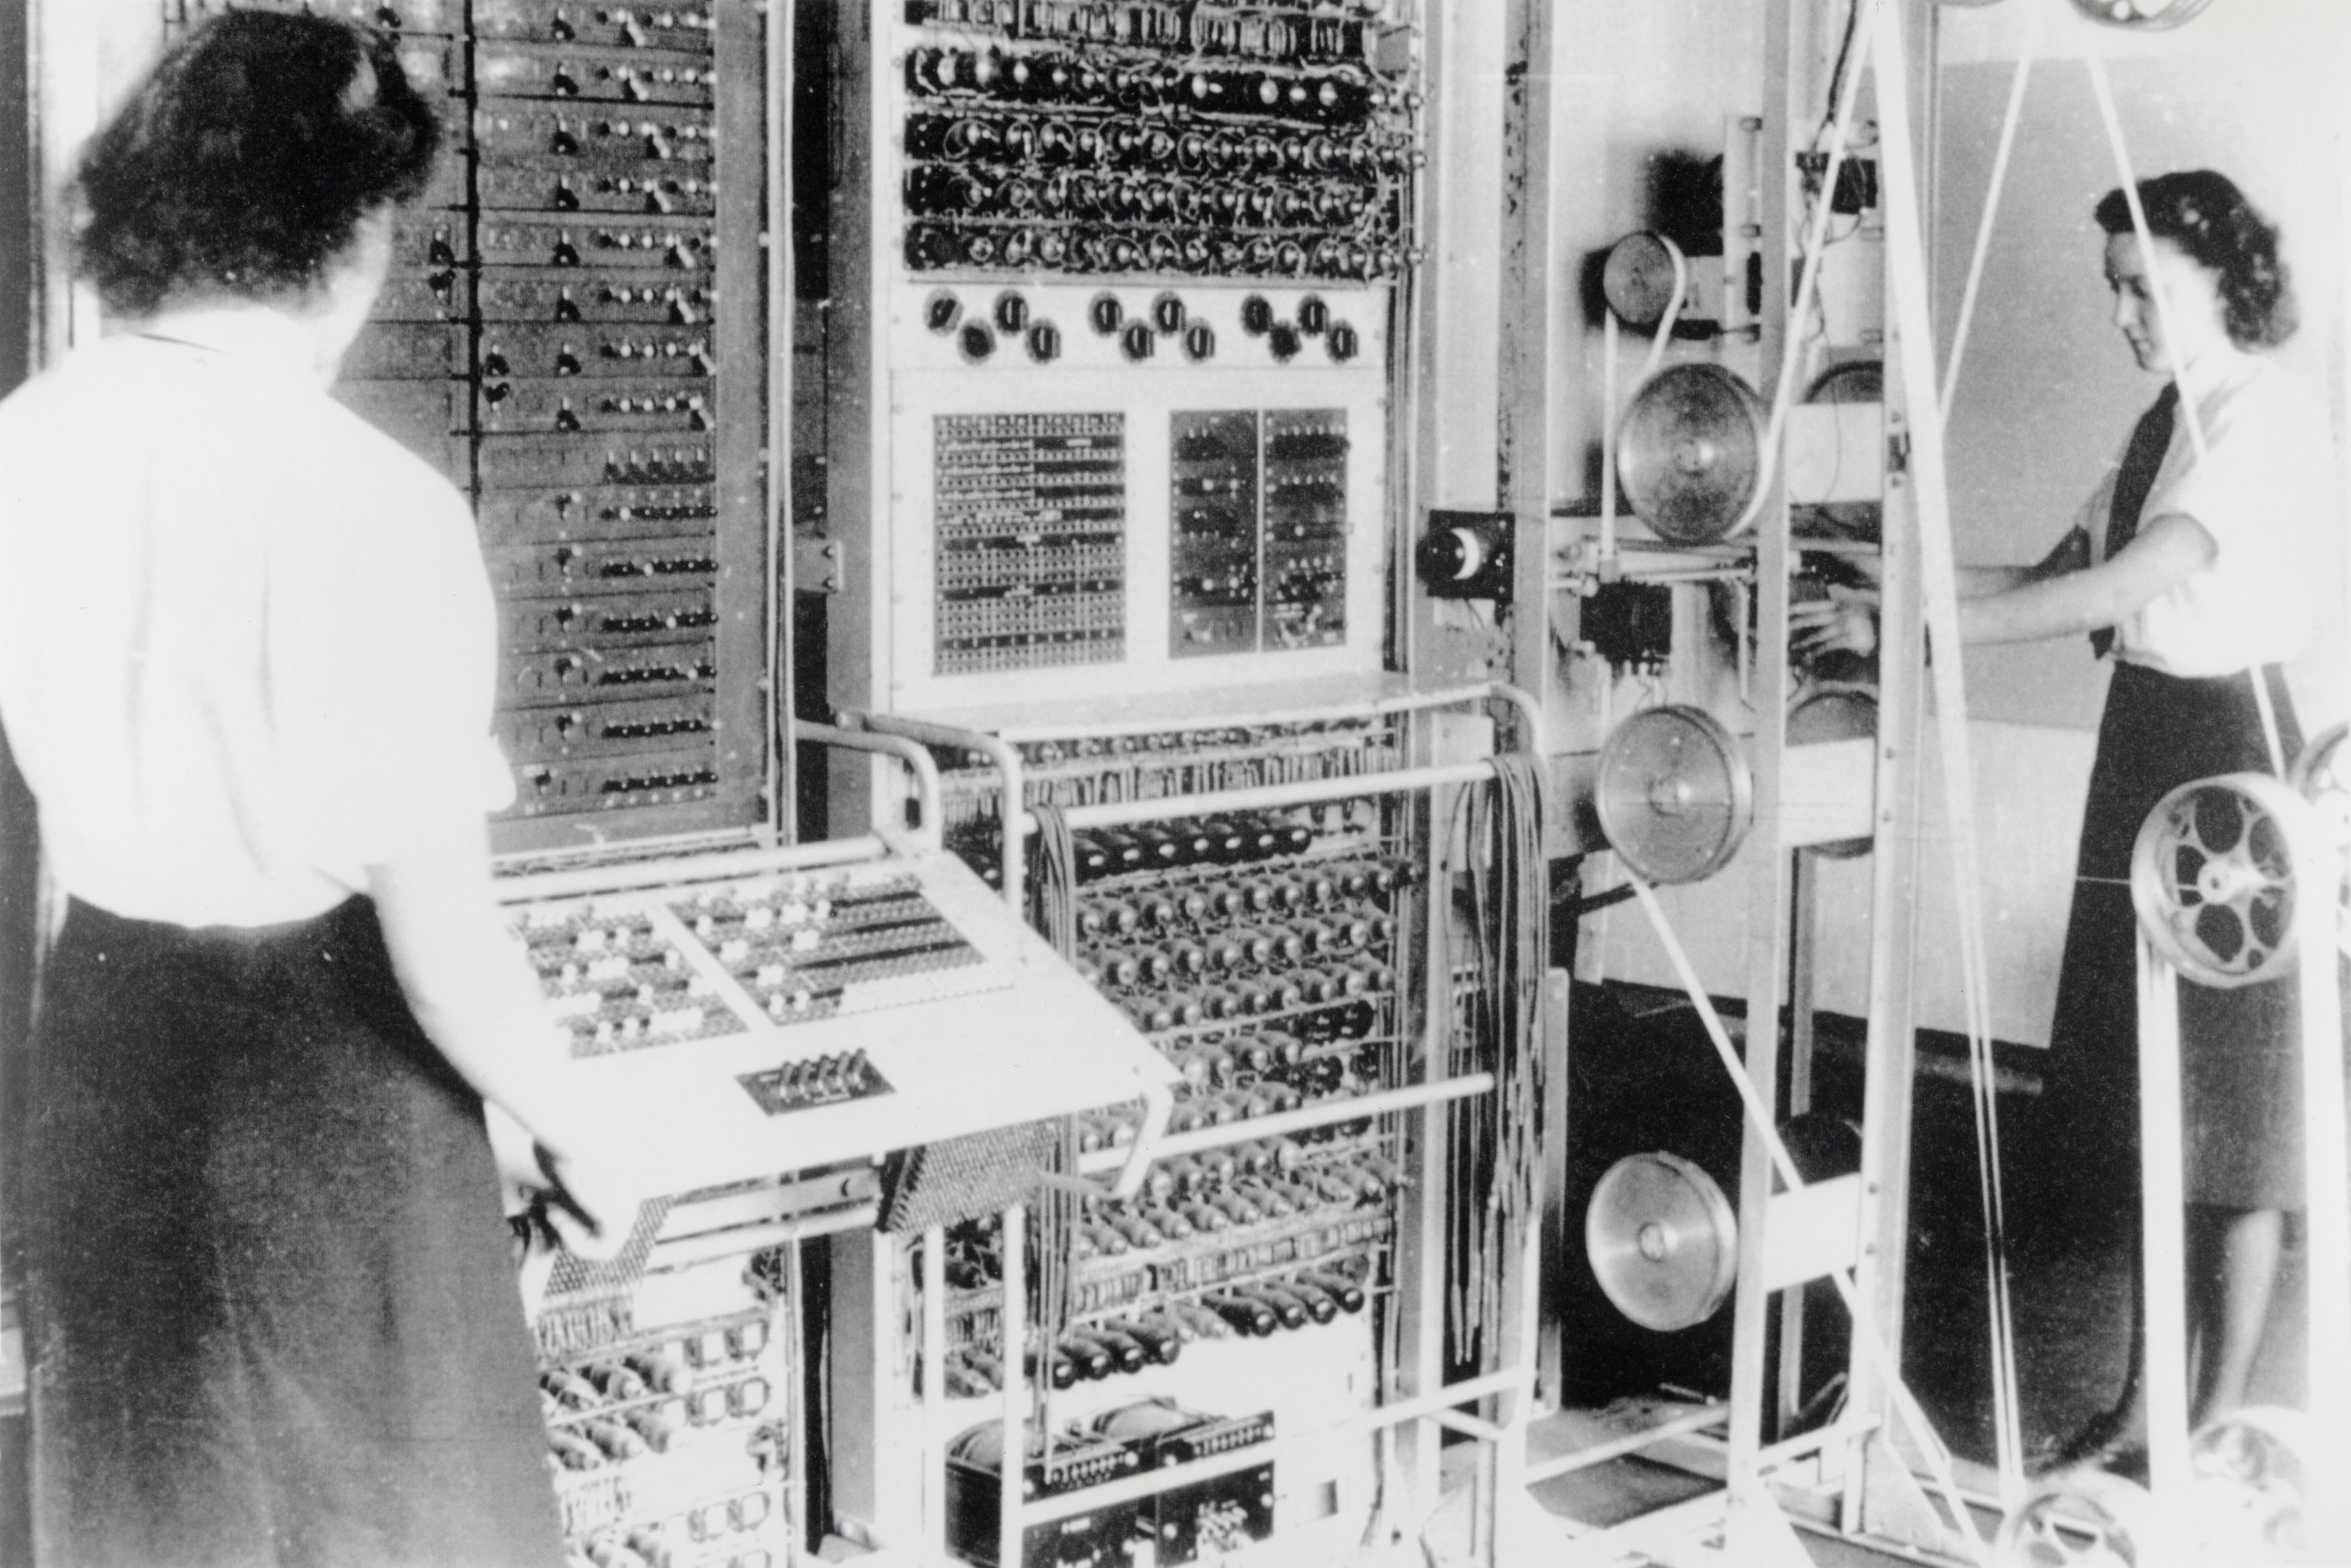
\includegraphics[width=\linewidth]{paper/images/colossus.jpg}
			\end{minipage}
		}
	\end{center}
\end{frame}

\begin{frame}[fragile]{Acknowledgments}
	\begin{itemize}
		\item Marian Rejewski, Jerzy Różycki, and Henryk Zygalski
		      \pause
		      \vspace{0.5em}
		\item Alan Turing, Gordon Welchman, Harold Keen, Hugh Alexander, and members of the Women's Royal Naval Service
		      \pause
		      \vspace{0.5em}
		\item Tony Sale, John Harper, Steve Hosgood, Graham Ellsbury, Andrew Martin, Dermot Turing, David Kenyon
		      and historians at Bletchley Park
		      \pause
		      \vspace{0.5em}
		\item Donald Davies and John Wright
		      \pause
		      \vspace{0.5em}
		\item Members of the committee and my advisor Christophe Hauser
		      \pause
		      \vspace{0.5em}
		\item Countless others
	\end{itemize}
\end{frame}

\begin{frame}[fragile]{Academic Contributions}
	\begin{enumerate}
		\item Present a chronological compendium of cryptographic attacks on Enigma -- focused on mathematically inclined readers
		      \pause
		      \vspace{5mm}
		\item Contribute code for analyzing attacks on Enigma
		      \pause
		      \vspace{5mm}

		\item {\bf{Analyze the Bombe through the lens of modern mathematics and simulation}}
	\end{enumerate}
\end{frame}

\begin{frame}[fragile]{Thesis Overview}
	\begin{itemize}
		\item Chapter \texttt{I} (The Enigma)
		      \vspace{1em}
		      \begin{itemize}
			      \setlength\itemsep{1em}
			      \item Key space
			      \item Enigma as a permutation
		      \end{itemize}
	\end{itemize}

\end{frame}

\begin{frame}[fragile]{Thesis Overview}
	\begin{itemize}

		\item Chapter \texttt{II} (The Polish Bomba)
		      \vspace{1em}
		      \begin{itemize}
			      \setlength\itemsep{1em}
			      \item Recovering Enigma wirings
			      \item The Grill Method
			      \item The Clock Method
			      \item The Cyclometer
			      \item Bomba Kryptologiczna
			      \item Zygalksi sheets
		      \end{itemize}
	\end{itemize}

\end{frame}


\begin{frame}[fragile]{Thesis Overview}
	\begin{itemize}
		\item Chapter \texttt{III} (The Turing-Welchman Bombe)
		      \vspace{1em}
		      \begin{itemize}
			      \setlength\itemsep{1em}
			      \item The Bombe
			      \item Diagonal board
			      \item Machine gun
			      \item Consecutive stecker knock out
			      \item Banburismus
		      \end{itemize}
	\end{itemize}

\end{frame}

\begin{frame}[fragile]{Thesis Overview}
	\begin{itemize}
		\item Chapter \texttt{IV} (Stops)
		      \vspace{1em}
		      \begin{itemize}
			      \setlength\itemsep{1em}
			      \item Turing's model
			      \item Development of a new cycle type model
			      \item H-M factor
		      \end{itemize}
	\end{itemize}

\end{frame}

\begin{frame}[fragile]{Presentation Overview}
	\begin{enumerate}
		\item The Enigma machine (Chapter \texttt{I})
		      \pause
		      \vspace{5mm}
		\item The Turing-Welchman Bombe (Chapter \texttt{III})
		      \pause
		      \vspace{5mm}

		\item Analysis of the Bombe (Chapter \texttt{IV})
	\end{enumerate}

\end{frame}


\part{}

\section{The Enigma}

\begin{frame}[fragile]{}
	\Huge
	\begin{center}
		The Enigma
	\end{center}
\end{frame}

\begin{frame}[fragile]{The Machine}
	\Huge
	\begin{center}
		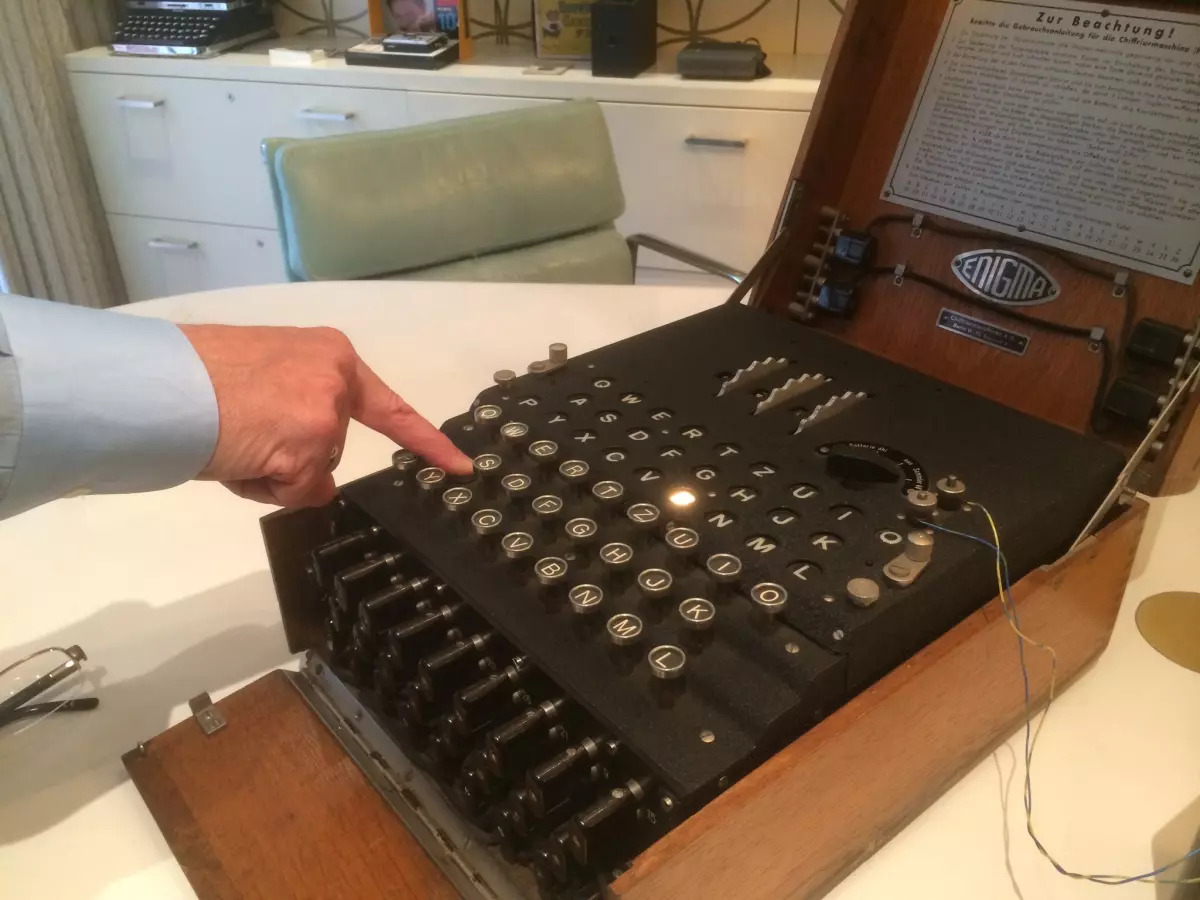
\includegraphics[scale=0.2]{paper/images/enigma.jpg}
	\end{center}
\end{frame}

\begin{frame}[fragile]{Overview}
	\begin{center}
		\scalebox{1}{
			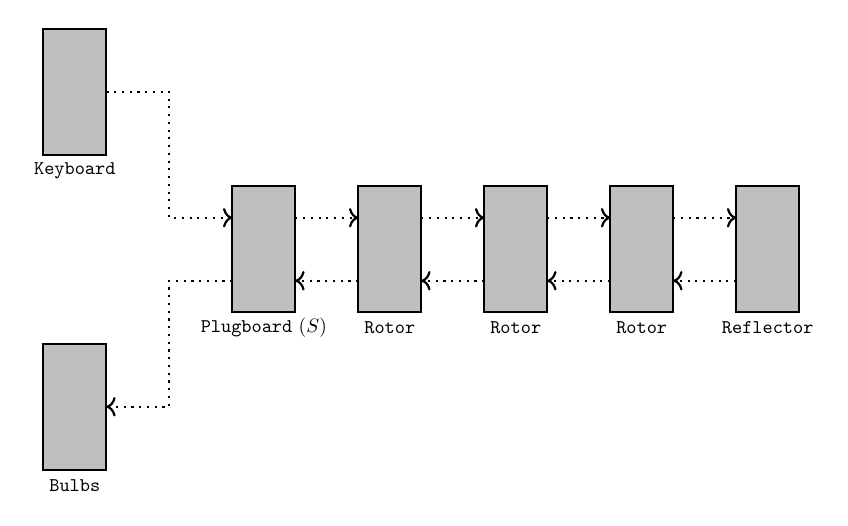
\begin{tikzpicture}[thick, scale=0.4, every node/.style={scale=0.7}]
				\draw[fill=lightgray] (0+5-14, 0+2+5) rectangle (2+5-14,4+2+5) node[midway] {};
				\node at (0+5+1-14, 0+2-0.5+5) {\texttt{Keyboard}};

				\draw[fill=lightgray] (0+5-14, 0+2-5) rectangle (2+5-14,4+2-5) node[midway] {};
				\node at (0+5+1-14, 0+2-0.5-5) {\texttt{Bulbs}};

				\draw[fill=lightgray] (0+5-8, 0+2) rectangle (2+5-8,4+2) node[midway] {};
				\node at (0+5+1-8, 0+2-0.5) {\texttt{Plugboard} ($S$)};

				\draw[fill=lightgray] (0+5, 0+2) rectangle (2+5,4+2) node[midway] {};
				\node at (0+5+1, 0+2-0.5) {\texttt{Rotor}};

				\draw[fill=lightgray] (0+5+4, 0+2) rectangle (2+5+4,4+2) node[midway] {};
				\node at (0+5+1+4, 0+2-0.5) {\texttt{Rotor}};

				\draw[fill=lightgray] (0+5+8, 0+2) rectangle (2+5+8,4+2) node[midway] {};
				\node at (0+5+1+8, 0+2-0.5) {\texttt{Reflector}};

				\draw[fill=lightgray] (0+5-4, 0+2) rectangle (2+5-4,4+2) node[midway] {};
				\node at (0+5+1-4, 0+2-0.5) {\texttt{Rotor}};

				\draw[->,dotted] (0+5-14+2, 0+2+5+2) -- (0+5-10, 0+2+5+2)
				-- (0+5-10, 0+2+5-2) -- (0+5-8, 0+2+5-2);

				\draw[->,dotted] (0+5-6, 0+2+5-2) -- (0+5-4, 0+2+5-2);
				\draw[->,dotted] (0+5-2, 0+2+5-2) -- (0+5, 0+2+5-2);
				\draw[->,dotted] (0+5+2, 0+2+5-2) -- (0+5+4, 0+2+5-2);
				\draw[->,dotted] (0+5+6, 0+2+5-2) -- (0+5+8, 0+2+5-2);

				\draw[->,dotted] (0+5+8, 0+2+5-4) -- (0+5+6, 0+2+5-4);
				\draw[->,dotted] (0+5+4, 0+2+5-4) -- (0+5+2, 0+2+5-4);
				\draw[->,dotted] (0+5, 0+2+5-4) -- (0+5-2, 0+2+5-4);
				\draw[->,dotted] (0+5-4, 0+2+5-4) -- (0+5-6, 0+2+5-4);

				\draw[->,dotted]  (0+5-8, 0+2+5-4) -- (0+5-10, 0+2+5-4)
				-- (0+5-10, 0+2+5-8) -- (0+5-14+2, 0+2+5-8) ;


			\end{tikzpicture}
		}
	\end{center}
\end{frame}

\begin{frame}[fragile]{Overview}
	\begin{center}
		\scalebox{1}{
			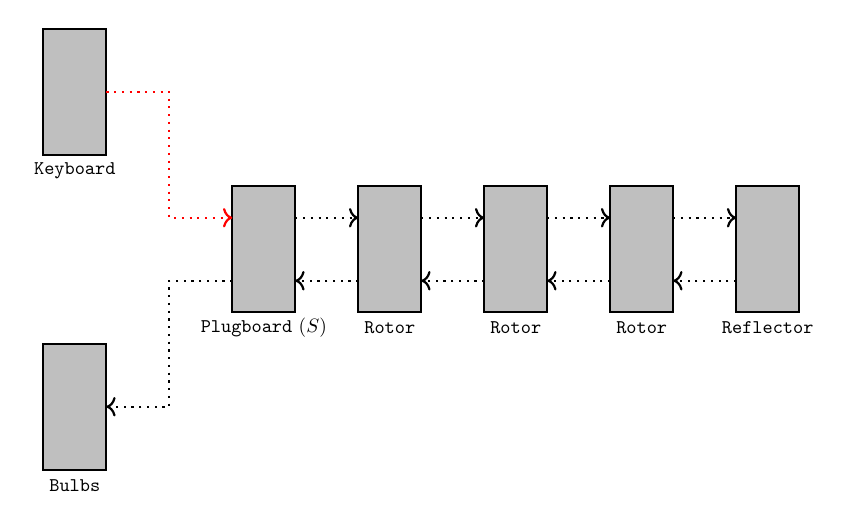
\begin{tikzpicture}[thick, scale=0.4, every node/.style={scale=0.7}]
				\draw[fill=lightgray] (0+5-14, 0+2+5) rectangle (2+5-14,4+2+5) node[midway] {};
				\node at (0+5+1-14, 0+2-0.5+5) {\texttt{Keyboard}};

				\draw[fill=lightgray] (0+5-14, 0+2-5) rectangle (2+5-14,4+2-5) node[midway] {};
				\node at (0+5+1-14, 0+2-0.5-5) {\texttt{Bulbs}};

				\draw[fill=lightgray] (0+5-8, 0+2) rectangle (2+5-8,4+2) node[midway] {};
				\node at (0+5+1-8, 0+2-0.5) {\texttt{Plugboard} ($S$)};

				\draw[fill=lightgray] (0+5, 0+2) rectangle (2+5,4+2) node[midway] {};
				\node at (0+5+1, 0+2-0.5) {\texttt{Rotor}};

				\draw[fill=lightgray] (0+5+4, 0+2) rectangle (2+5+4,4+2) node[midway] {};
				\node at (0+5+1+4, 0+2-0.5) {\texttt{Rotor}};

				\draw[fill=lightgray] (0+5+8, 0+2) rectangle (2+5+8,4+2) node[midway] {};
				\node at (0+5+1+8, 0+2-0.5) {\texttt{Reflector}};

				\draw[fill=lightgray] (0+5-4, 0+2) rectangle (2+5-4,4+2) node[midway] {};
				\node at (0+5+1-4, 0+2-0.5) {\texttt{Rotor}};

				\draw[->, red ,dotted] (0+5-14+2, 0+2+5+2) -- (0+5-10, 0+2+5+2)
				-- (0+5-10, 0+2+5-2) -- (0+5-8, 0+2+5-2);

				\draw[->,dotted] (0+5-6, 0+2+5-2) -- (0+5-4, 0+2+5-2);
				\draw[->,dotted] (0+5-2, 0+2+5-2) -- (0+5, 0+2+5-2);
				\draw[->,dotted] (0+5+2, 0+2+5-2) -- (0+5+4, 0+2+5-2);
				\draw[->,dotted] (0+5+6, 0+2+5-2) -- (0+5+8, 0+2+5-2);

				\draw[->,dotted] (0+5+8, 0+2+5-4) -- (0+5+6, 0+2+5-4);
				\draw[->,dotted] (0+5+4, 0+2+5-4) -- (0+5+2, 0+2+5-4);
				\draw[->,dotted] (0+5, 0+2+5-4) -- (0+5-2, 0+2+5-4);
				\draw[->,dotted] (0+5-4, 0+2+5-4) -- (0+5-6, 0+2+5-4);

				\draw[->,dotted]  (0+5-8, 0+2+5-4) -- (0+5-10, 0+2+5-4)
				-- (0+5-10, 0+2+5-8) -- (0+5-14+2, 0+2+5-8) ;


			\end{tikzpicture}
		}
	\end{center}
\end{frame}

\begin{frame}[fragile]{The Plugboard}
	\begin{center}
		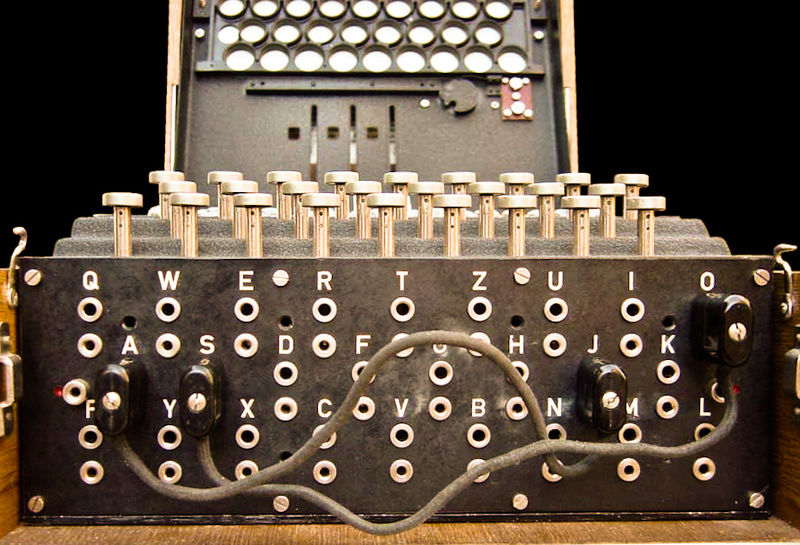
\includegraphics[]{paper/images/plugboard.jpg}
	\end{center}
\end{frame}

\begin{frame}[fragile]{Overview}
	\begin{center}
		\scalebox{1}{
			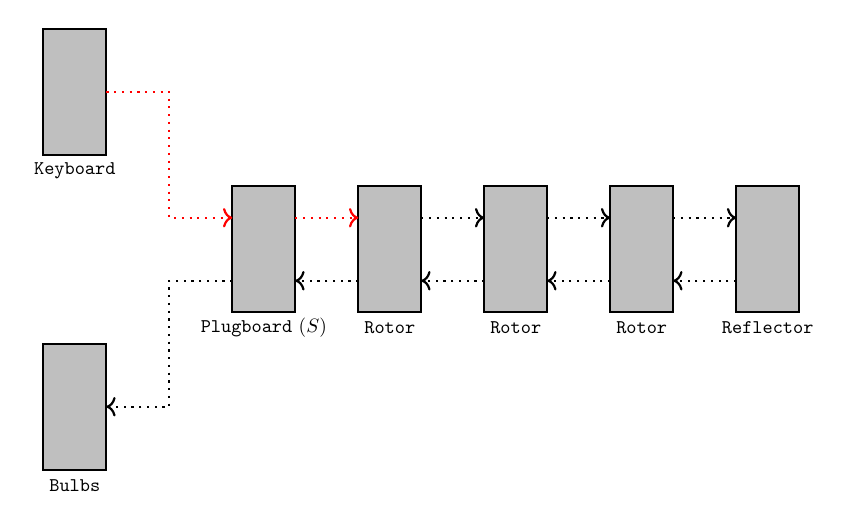
\begin{tikzpicture}[thick, scale=0.4, every node/.style={scale=0.7}]
				\draw[fill=lightgray] (0+5-14, 0+2+5) rectangle (2+5-14,4+2+5) node[midway] {};
				\node at (0+5+1-14, 0+2-0.5+5) {\texttt{Keyboard}};

				\draw[fill=lightgray] (0+5-14, 0+2-5) rectangle (2+5-14,4+2-5) node[midway] {};
				\node at (0+5+1-14, 0+2-0.5-5) {\texttt{Bulbs}};

				\draw[fill=lightgray] (0+5-8, 0+2) rectangle (2+5-8,4+2) node[midway] {};
				\node at (0+5+1-8, 0+2-0.5) {\texttt{Plugboard} ($S$)};

				\draw[fill=lightgray] (0+5, 0+2) rectangle (2+5,4+2) node[midway] {};
				\node at (0+5+1, 0+2-0.5) {\texttt{Rotor}};

				\draw[fill=lightgray] (0+5+4, 0+2) rectangle (2+5+4,4+2) node[midway] {};
				\node at (0+5+1+4, 0+2-0.5) {\texttt{Rotor}};

				\draw[fill=lightgray] (0+5+8, 0+2) rectangle (2+5+8,4+2) node[midway] {};
				\node at (0+5+1+8, 0+2-0.5) {\texttt{Reflector}};

				\draw[fill=lightgray] (0+5-4, 0+2) rectangle (2+5-4,4+2) node[midway] {};
				\node at (0+5+1-4, 0+2-0.5) {\texttt{Rotor}};

				\draw[->, red,dotted] (0+5-14+2, 0+2+5+2) -- (0+5-10, 0+2+5+2)
				-- (0+5-10, 0+2+5-2) -- (0+5-8, 0+2+5-2);

				\draw[->, red,dotted] (0+5-6, 0+2+5-2) -- (0+5-4, 0+2+5-2);
				\draw[->,dotted] (0+5-2, 0+2+5-2) -- (0+5, 0+2+5-2);
				\draw[->,dotted] (0+5+2, 0+2+5-2) -- (0+5+4, 0+2+5-2);
				\draw[->,dotted] (0+5+6, 0+2+5-2) -- (0+5+8, 0+2+5-2);

				\draw[->,dotted] (0+5+8, 0+2+5-4) -- (0+5+6, 0+2+5-4);
				\draw[->,dotted] (0+5+4, 0+2+5-4) -- (0+5+2, 0+2+5-4);
				\draw[->,dotted] (0+5, 0+2+5-4) -- (0+5-2, 0+2+5-4);
				\draw[->,dotted] (0+5-4, 0+2+5-4) -- (0+5-6, 0+2+5-4);

				\draw[->,dotted]  (0+5-8, 0+2+5-4) -- (0+5-10, 0+2+5-4)
				-- (0+5-10, 0+2+5-8) -- (0+5-14+2, 0+2+5-8) ;


			\end{tikzpicture}
		}
	\end{center}
\end{frame}

\begin{frame}[fragile]{The Rotors}
	\begin{center}
		\scalebox{0.9}{
			\begin{minipage}{0.48\textwidth}
				\centering
				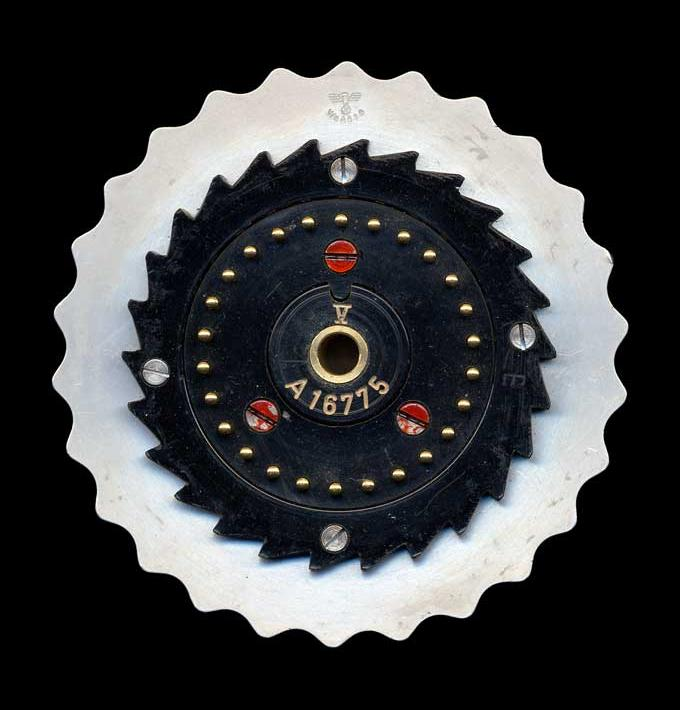
\includegraphics[width=\linewidth]{paper/images/entry.jpg}
			\end{minipage}%
			\hfill
			\begin{minipage}{0.48\textwidth}
				\centering
				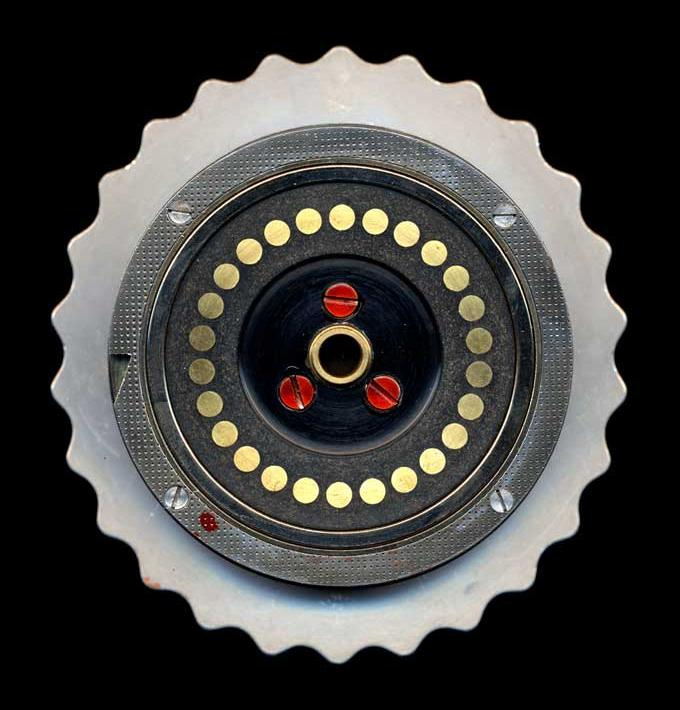
\includegraphics[width=\linewidth]{paper/images/exit.jpg}
			\end{minipage}
		}
	\end{center}
\end{frame}


\begin{frame}[fragile]{The Rotors}
	\begin{center}
		\animategraphics[loop,width=10cm]{10}{paper/images/ratchet_gif/ratchet_gif-}{0}{59}
	\end{center}
\end{frame}


% \begin{frame}[fragile]{The Rotors}
% 	\begin{figure}
% 		\centering
% 		\[\left(
% 			\begin{array}{llllllllllllllllllllllllll}
% 					\texttt{A} & \texttt{B} & \texttt{C} & \texttt{D} &
% 					\texttt{E} & \texttt{F} & \texttt{G} & \texttt{H} &
% 					\texttt{I} & \texttt{J} & \texttt{K} & \texttt{L} &
% 					\texttt{M} & \texttt{N} & \texttt{O} & \texttt{P} &
% 					\texttt{Q} & \texttt{R} & \texttt{S} & \texttt{T} &
% 					\texttt{U} & \texttt{V} & \texttt{W} & \texttt{X} &
% 					\texttt{Y} & \texttt{Z}                             \\
% 					\texttt{B} & \texttt{C} & \texttt{D} &
% 					\texttt{E} & \texttt{F} & \texttt{G} & \texttt{H} &
% 					\texttt{I} & \texttt{J} & \texttt{K} & \texttt{L} &
% 					\texttt{M} & \texttt{N} & \texttt{O} & \texttt{P} &
% 					\texttt{Q} & \texttt{R} & \texttt{S} & \texttt{T} &
% 					\texttt{U} & \texttt{V} & \texttt{W} & \texttt{X} &
% 					\texttt{Y} & \texttt{Z} & \texttt{A}
% 				\end{array}
% 			\right)\]
% 		\caption{The Caesar Permutation $P$}
% 	\end{figure}
% \end{frame}


% \begin{frame}[fragile]{The Rotors}
% 	After $r$ steps forward we have,
% 	\[
% 		{P^{-r}}N{P^{r}}.
% 	\]
% \end{frame}

\begin{frame}[fragile]{Overview}
	\begin{center}
		\scalebox{1}{
			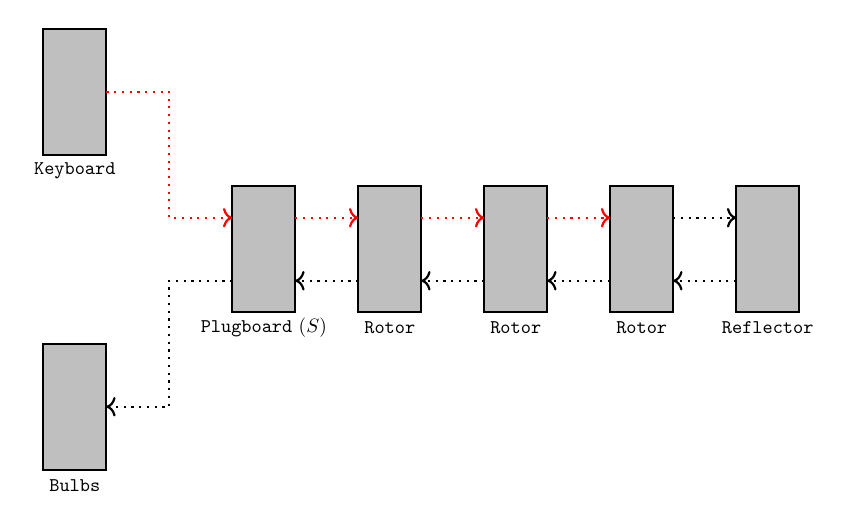
\begin{tikzpicture}[thick, scale=0.4, every node/.style={scale=0.7}]
				\draw[fill=lightgray] (0+5-14, 0+2+5) rectangle (2+5-14,4+2+5) node[midway] {};
				\node at (0+5+1-14, 0+2-0.5+5) {\texttt{Keyboard}};

				\draw[fill=lightgray] (0+5-14, 0+2-5) rectangle (2+5-14,4+2-5) node[midway] {};
				\node at (0+5+1-14, 0+2-0.5-5) {\texttt{Bulbs}};

				\draw[fill=lightgray] (0+5-8, 0+2) rectangle (2+5-8,4+2) node[midway] {};
				\node at (0+5+1-8, 0+2-0.5) {\texttt{Plugboard} ($S$)};

				\draw[fill=lightgray] (0+5, 0+2) rectangle (2+5,4+2) node[midway] {};
				\node at (0+5+1, 0+2-0.5) {\texttt{Rotor}};

				\draw[fill=lightgray] (0+5+4, 0+2) rectangle (2+5+4,4+2) node[midway] {};
				\node at (0+5+1+4, 0+2-0.5) {\texttt{Rotor}};

				\draw[fill=lightgray] (0+5+8, 0+2) rectangle (2+5+8,4+2) node[midway] {};
				\node at (0+5+1+8, 0+2-0.5) {\texttt{Reflector}};

				\draw[fill=lightgray] (0+5-4, 0+2) rectangle (2+5-4,4+2) node[midway] {};
				\node at (0+5+1-4, 0+2-0.5) {\texttt{Rotor}};

				\draw[->, red,dotted] (0+5-14+2, 0+2+5+2) -- (0+5-10, 0+2+5+2)
				-- (0+5-10, 0+2+5-2) -- (0+5-8, 0+2+5-2);

				\draw[->, red,dotted] (0+5-6, 0+2+5-2) -- (0+5-4, 0+2+5-2);
				\draw[->, red,dotted] (0+5-2, 0+2+5-2) -- (0+5, 0+2+5-2);
				\draw[->, red,dotted] (0+5+2, 0+2+5-2) -- (0+5+4, 0+2+5-2);
				\draw[->,dotted] (0+5+6, 0+2+5-2) -- (0+5+8, 0+2+5-2);

				\draw[->,dotted] (0+5+8, 0+2+5-4) -- (0+5+6, 0+2+5-4);
				\draw[->,dotted] (0+5+4, 0+2+5-4) -- (0+5+2, 0+2+5-4);
				\draw[->,dotted] (0+5, 0+2+5-4) -- (0+5-2, 0+2+5-4);
				\draw[->,dotted] (0+5-4, 0+2+5-4) -- (0+5-6, 0+2+5-4);

				\draw[->,dotted]  (0+5-8, 0+2+5-4) -- (0+5-10, 0+2+5-4)
				-- (0+5-10, 0+2+5-8) -- (0+5-14+2, 0+2+5-8) ;


			\end{tikzpicture}
		}
	\end{center}
\end{frame}


\begin{frame}[fragile]{The Rotors}
	\begin{center}
		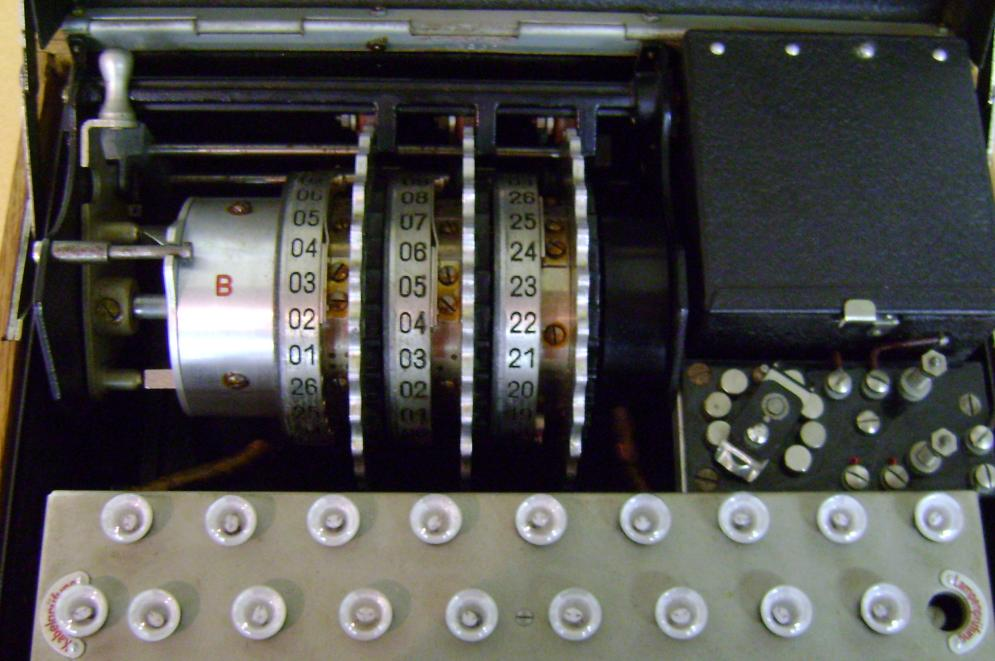
\includegraphics[scale=0.28]{paper/images/internals_rotor.jpg}
	\end{center}
\end{frame}

\begin{frame}[fragile]{The Rotors}
	\begin{center}
		\animategraphics[loop,width=10cm]{10}{paper/images/turnover_gif/double_step_gif-}{0}{262}
	\end{center}
\end{frame}


\begin{frame}[fragile]{Overview}
	\begin{center}
		\scalebox{1}{
			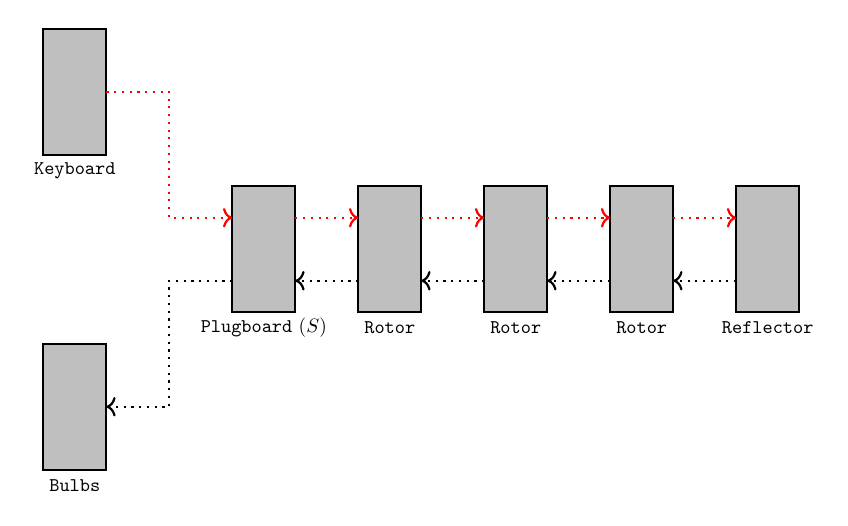
\begin{tikzpicture}[thick, scale=0.4, every node/.style={scale=0.7}]
				\draw[fill=lightgray] (0+5-14, 0+2+5) rectangle (2+5-14,4+2+5) node[midway] {};
				\node at (0+5+1-14, 0+2-0.5+5) {\texttt{Keyboard}};

				\draw[fill=lightgray] (0+5-14, 0+2-5) rectangle (2+5-14,4+2-5) node[midway] {};
				\node at (0+5+1-14, 0+2-0.5-5) {\texttt{Bulbs}};

				\draw[fill=lightgray] (0+5-8, 0+2) rectangle (2+5-8,4+2) node[midway] {};
				\node at (0+5+1-8, 0+2-0.5) {\texttt{Plugboard} ($S$)};

				\draw[fill=lightgray] (0+5, 0+2) rectangle (2+5,4+2) node[midway] {};
				\node at (0+5+1, 0+2-0.5) {\texttt{Rotor}};

				\draw[fill=lightgray] (0+5+4, 0+2) rectangle (2+5+4,4+2) node[midway] {};
				\node at (0+5+1+4, 0+2-0.5) {\texttt{Rotor}};

				\draw[fill=lightgray] (0+5+8, 0+2) rectangle (2+5+8,4+2) node[midway] {};
				\node at (0+5+1+8, 0+2-0.5) {\texttt{Reflector}};

				\draw[fill=lightgray] (0+5-4, 0+2) rectangle (2+5-4,4+2) node[midway] {};
				\node at (0+5+1-4, 0+2-0.5) {\texttt{Rotor}};

				\draw[->, red,dotted] (0+5-14+2, 0+2+5+2) -- (0+5-10, 0+2+5+2)
				-- (0+5-10, 0+2+5-2) -- (0+5-8, 0+2+5-2);

				\draw[->, red,dotted] (0+5-6, 0+2+5-2) -- (0+5-4, 0+2+5-2);
				\draw[->, red,dotted] (0+5-2, 0+2+5-2) -- (0+5, 0+2+5-2);
				\draw[->, red,dotted] (0+5+2, 0+2+5-2) -- (0+5+4, 0+2+5-2);
				\draw[->, red,dotted] (0+5+6, 0+2+5-2) -- (0+5+8, 0+2+5-2);

				\draw[->,dotted] (0+5+8, 0+2+5-4) -- (0+5+6, 0+2+5-4);
				\draw[->,dotted] (0+5+4, 0+2+5-4) -- (0+5+2, 0+2+5-4);
				\draw[->,dotted] (0+5, 0+2+5-4) -- (0+5-2, 0+2+5-4);
				\draw[->,dotted] (0+5-4, 0+2+5-4) -- (0+5-6, 0+2+5-4);

				\draw[->,dotted]  (0+5-8, 0+2+5-4) -- (0+5-10, 0+2+5-4)
				-- (0+5-10, 0+2+5-8) -- (0+5-14+2, 0+2+5-8) ;


			\end{tikzpicture}
		}
	\end{center}
\end{frame}


\begin{frame}[fragile]{The Reflector}
	\begin{center}
		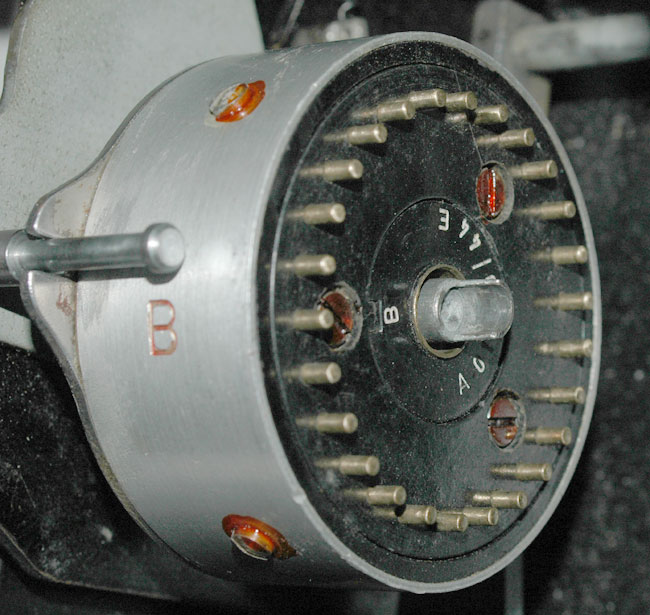
\includegraphics[scale=0.28]{paper/images/reflector.jpg}
	\end{center}
\end{frame}

\begin{frame}[fragile]{Overview}
	\begin{center}
		\scalebox{1}{
			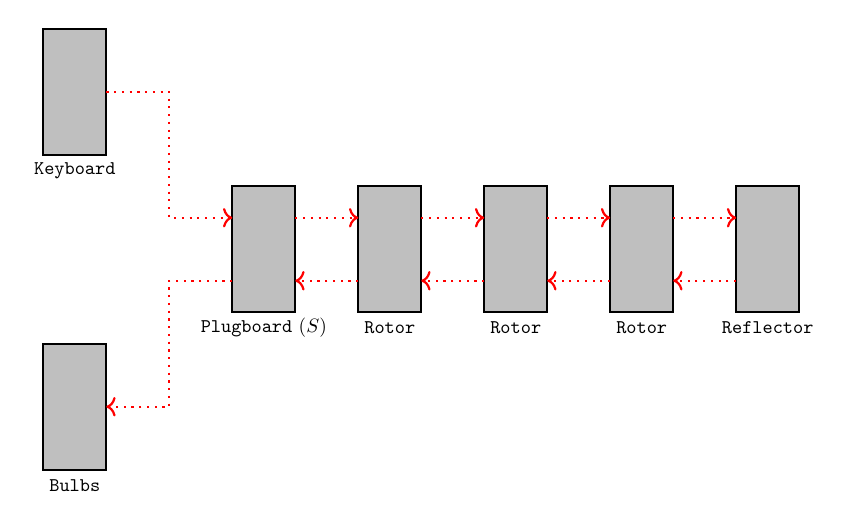
\begin{tikzpicture}[thick, scale=0.4, every node/.style={scale=0.7}]
				\draw[fill=lightgray] (0+5-14, 0+2+5) rectangle (2+5-14,4+2+5) node[midway] {};
				\node at (0+5+1-14, 0+2-0.5+5) {\texttt{Keyboard}};

				\draw[fill=lightgray] (0+5-14, 0+2-5) rectangle (2+5-14,4+2-5) node[midway] {};
				\node at (0+5+1-14, 0+2-0.5-5) {\texttt{Bulbs}};

				\draw[fill=lightgray] (0+5-8, 0+2) rectangle (2+5-8,4+2) node[midway] {};
				\node at (0+5+1-8, 0+2-0.5) {\texttt{Plugboard} ($S$)};

				\draw[fill=lightgray] (0+5, 0+2) rectangle (2+5,4+2) node[midway] {};
				\node at (0+5+1, 0+2-0.5) {\texttt{Rotor}};

				\draw[fill=lightgray] (0+5+4, 0+2) rectangle (2+5+4,4+2) node[midway] {};
				\node at (0+5+1+4, 0+2-0.5) {\texttt{Rotor}};

				\draw[fill=lightgray] (0+5+8, 0+2) rectangle (2+5+8,4+2) node[midway] {};
				\node at (0+5+1+8, 0+2-0.5) {\texttt{Reflector}};

				\draw[fill=lightgray] (0+5-4, 0+2) rectangle (2+5-4,4+2) node[midway] {};
				\node at (0+5+1-4, 0+2-0.5) {\texttt{Rotor}};

				\draw[->, red,dotted] (0+5-14+2, 0+2+5+2) -- (0+5-10, 0+2+5+2)
				-- (0+5-10, 0+2+5-2) -- (0+5-8, 0+2+5-2);

				\draw[->, red,dotted] (0+5-6, 0+2+5-2) -- (0+5-4, 0+2+5-2);
				\draw[->, red,dotted] (0+5-2, 0+2+5-2) -- (0+5, 0+2+5-2);
				\draw[->, red,dotted] (0+5+2, 0+2+5-2) -- (0+5+4, 0+2+5-2);
				\draw[->, red,dotted] (0+5+6, 0+2+5-2) -- (0+5+8, 0+2+5-2);

				\draw[->, red,dotted] (0+5+8, 0+2+5-4) -- (0+5+6, 0+2+5-4);
				\draw[->, red,dotted] (0+5+4, 0+2+5-4) -- (0+5+2, 0+2+5-4);
				\draw[->, red,dotted] (0+5, 0+2+5-4) -- (0+5-2, 0+2+5-4);
				\draw[->, red,dotted] (0+5-4, 0+2+5-4) -- (0+5-6, 0+2+5-4);

				\draw[->, red,dotted]  (0+5-8, 0+2+5-4) -- (0+5-10, 0+2+5-4)
				-- (0+5-10, 0+2+5-8) -- (0+5-14+2, 0+2+5-8) ;


			\end{tikzpicture}
		}
	\end{center}
\end{frame}

% \begin{frame}{Enigma Permutation}
% 	Then an Enigma permutation takes the form,
% 	\begin{center}
% 		$\pi_0 = S^{-1}N^{-1}M^{-1}L^{-1}RLMNS$
% 	\end{center}
% \end{frame}

% \begin{frame}{Enigma Permutation}
% 	After $i$ steps, without turnover,
% 	\begin{center}
% 		$\pi_i = S^{-1}P^{i}N^{-1}P^{-i}M^{-1}L^{-1}RLMP^{-i}NP^{i}S$
% 	\end{center}
% \end{frame}

% \begin{frame}{Enigma Permutation}
% 	We note,
% 	\begin{align*}
% 		\pi_i & = S^{-1}P^{i}N^{-1}P^{-i}M^{-1}L^{-1}RLMP^{-i}NP^{i}S
% 		\\ &= (LMP^{-i}NP^{i}S)^{-1}R(LMP^{-i}NP^{i}S)
% 	\end{align*}
% \end{frame}

\begin{frame}{Enigma Permutation}
	\begin{theorem}
		$\forall\text{ }\alpha, \beta \in S_n$ we have
		\begin{center}
			$\alpha$ and $\beta$ are conjugates $\iff$ $\alpha$ and $\beta$
			have the same cycle type.
		\end{center}
	\end{theorem}

\end{frame}

\begin{frame}{Enigma Permutation}
	The reflector is composed of $13$ disjoint transpositions. Then, at any given position,
	\vspace{1em}
	\begin{enumerate}

		\item The Enigma is an involution -- $\forall \text{ }x\in\mathbb{N}_n$, $\pi_i(\pi_i(x)) = x$
		      \vspace{1em}
		\item The Enigma has no fixed points -- $\forall\text{ }x\in\mathbb{N}_n$, $\pi_i(x) \ne x$
	\end{enumerate}
\end{frame}



\begin{frame}{Sending Messages}
	\begin{center}
		\begin{figure}[H]
			\begin{center}
				\resizebox{0.98\textwidth}{!}{
					\begin{tabular}{|c|c|c|c|}
						\hline
						\textbf{\emph{\texttt{Datum}}}        &
						\textbf{\emph{\texttt{Walzenlage}}}   &
						\textbf{\emph{\texttt{Ringstellung}}} &
						\textbf{\emph{\texttt{Steckerverbindungen}}}                                                                            \\
						% \textbf{\emph{\texttt{Grundstellung}}}
						% \\
						\hline
						\texttt{31.}                          & \texttt{IV V I}    & \texttt{21 15 16} & \texttt{KL IT FQ HY XC NP VZ JB SE OG} %                                          & \texttt{VAR}
						\\
						\texttt{30.}                          & \texttt{IV II III} & \texttt{26 14 11} & \texttt{ZN YO QB ER DK XU GP TV SJ LM} %                                          & \texttt{PAQ}
						\\
						\texttt{29.}                          & \texttt{II V IV}   & \texttt{19 09 24} & \texttt{ZU HL CQ WM OA PY EB TR DN VI} %                                         & \texttt{ZJB}
						\\
						$\vdots$                              & $\vdots$
						                                      & $\vdots$           & $\vdots$                                                   \\
						\hline
					\end{tabular}}
			\end{center}
			\caption{Mock Enigma key sheet}
			\label{fig:keysheet_early}
		\end{figure}
	\end{center}
\end{frame}

\begin{frame}{Sending Messages}
	When sending a message the operator was to use the following protocol
	\begin{enumerate}
		\item The operator sets up their machine according to the key sheet
		      \pause
		      \vspace{1em}
		\item A random window setting (\emph{Grundstellung}) is chosen and sent in plaintext
		      \pause
		      \vspace{1em}
		\item A random message key (\emph{Spruchschlüssel}) is chosen and the window setting (\emph{Grundstellung}) is used to encipher this message key
        		      \pause
		      \vspace{1em}
        \item Send the enciphered message key (\emph{Spruchschlüssel})
        		      \pause
		      \vspace{1em}
		\item The remainder of the message is enciphered using the message key (\emph{Spruchschlüssel}) and sent
	\end{enumerate}
\end{frame}

% DEMO ON ENIGMA MACHINE SIM


\begin{frame}{Sending Messages}
    On the 31st of the month we set 
    \begin{itemize}
        \item Rotor order to \texttt{IV V I}
        \item Ring setting to \texttt{21 15 16}
        \item Plugboard to \texttt{KL IT FQ HY XC NP VZ JB SE OG}
        \item Window setting to a random choice \texttt{XYZ}
    \end{itemize}
\end{frame}

\begin{frame}{Sending Messages}
We send
    \begin{center}
        \texttt{XYZ}
    \end{center}
\end{frame}

\begin{frame}{Sending Messages}
We encipher a random message key \texttt{ABC} as
    \begin{center}
        \texttt{FZK}
    \end{center}
\end{frame}

\begin{frame}{Sending Messages}
We send
    \begin{center}
        \texttt{XYZ FZK}
    \end{center}
\end{frame}

\begin{frame}{Sending Messages}
We change our window setting to \texttt{ABC} and encipher our message \texttt{HELLOXWORLD} as
    \begin{center}
        \texttt{BQAQMQCQPEX}
    \end{center}
\end{frame}

\begin{frame}{Sending Messages}
We send
    \begin{center}
        \texttt{XYZ FZK BQAQMQCQPEX}
    \end{center}
\end{frame}

\begin{frame}{Sending Messages}
    We recieve \texttt{XYZ FZK BQAQMQCQPEX} and set
    \begin{itemize}
        \item Rotor order to \texttt{IV V I}
        \item Ring setting to \texttt{21 15 16}
        \item Plugboard to \texttt{KL IT FQ HY XC NP VZ JB SE OG}
        \item Window setting to \texttt{XYZ}
    \end{itemize}
\end{frame}

\begin{frame}{Sending Messages}
We decipher \texttt{FZK} as
    \begin{center}
        \texttt{ABC}
    \end{center}
\end{frame}

\begin{frame}{Sending Messages}
We change our window setting to \texttt{ABC} and decipher our message \texttt{BQAQMQCQPEX} as
    \begin{center}
        \texttt{HELLOXWORLD}
    \end{center}
\end{frame}

% \subsection{Key Space}

% \begin{frame}[fragile]{Slide}
% \end{frame}

% \part{}

% \section{Group Theory and Permutations}

% \begin{frame}[fragile]{Slide}
% \end{frame}

% \subsection{Enigma as a Permutation}

% \begin{frame}[fragile]{Slide}
% \end{frame}

% \part{}
% \section{The Cyclometer}

% \subsection{Characteristics}
% \begin{frame}[fragile]{Slide}
% \end{frame}

% \subsection{The Cyclometer}
% \begin{frame}[fragile]{Slide}
% \end{frame}

\part{}
\section{The Turing-Welchman Bombe}

\begin{frame}[fragile]{}
	\Huge
	\begin{center}
		The Turing-Welchman Bombe
	\end{center}
\end{frame}

\begin{frame}[fragile]{Plaintext Attack}
	\begin{center}
		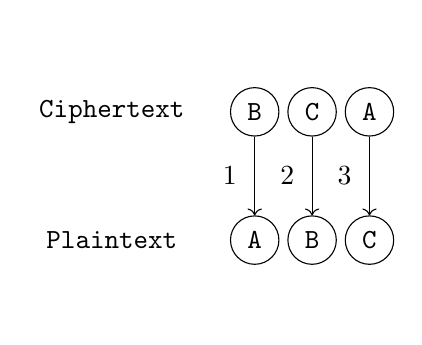
\begin{tikzpicture}[node distance=1cm, every node/.style={draw,
						circle, minimum height=0.1cm, minimum width=0.1cm}]

			% Centering the diagram
			\node (a1) [] {\texttt{B}};
			\node (a2) [right=0.1cm of a1] {\texttt{C}};
			\node (a3) [right=0.1cm of a2] {\texttt{A}};

			% Nodes for ciphertext
			\node (x1) [below=1cm of a1] {\texttt{A}};
			\node (x2) [below=1cm of a2] {\texttt{B}};
			\node (x3) [below=1cm of a3] {\texttt{C}};

			% Arrows for mapping
			\draw[->] (a1) -- (x1) node[midway, left, draw=none, fill=none] {1};
			\draw[->] (a2) -- (x2) node[midway, left, draw=none, fill=none] {2};
			\draw[->] (a3) -- (x3) node[midway, left, draw=none, fill=none] {3};

                 \node[draw=none] at ([xshift=-1.5cm]a1.west) {\texttt{Ciphertext }};
                 \node[draw=none] at ([xshift=-1.5cm]x1.west) {\texttt{Plaintext  }};

		\end{tikzpicture}
	\end{center}\blfootnote{For many examples we will switch to a $4$ letter alphabet.}
\end{frame}

\begin{frame}[fragile]{Plaintext Attack}
	\begin{center}
		$\pi_1(\texttt{B}) = {\texttt{A}}$\\
		\vspace{1em}
		$\pi_2(\texttt{C}) = {\texttt{B}}$\\
		\vspace{1em}
		$\pi_{3}(\texttt{A}) = {\texttt{C}}$\\
	\end{center}
\end{frame}

\begin{frame}[fragile]{Plaintext Attack}
	\begin{center}
		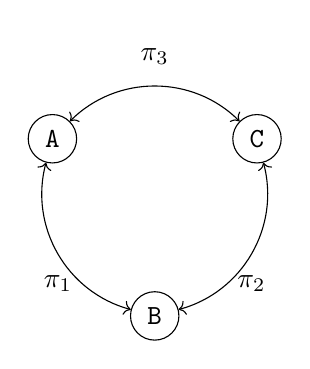
\begin{tikzpicture}[node distance=1cm, every node/.style={draw,
						circle, minimum height=0.1cm, minimum width=0.1cm}]
			\node (A) at (270-120:1.5) {$\texttt{A}$};
			\node (B) at (270:1.5) {$\texttt{B}$};
			\node (C) at (270+120:1.5) {$\texttt{C}$};

			\draw[<->, bend right=45] (A) to node[midway, draw=none, below] {$\pi_1$} (B);
			\draw[<->, bend right=45] (B) to node[midway, draw=none, below] {$\pi_2$} (C);
			\draw[<->, bend right=45] (C) to node[midway, draw=none, above] {$\pi_{3}$} (A);

		\end{tikzpicture}
	\end{center}
\end{frame}


\begin{frame}[fragile]{Plaintext Attack}
	Then our loop,
	\begin{center}
		$\pi_{3}\pi_2\pi_1$
	\end{center}
	has a fixed point at \texttt{A}.
\end{frame}

\begin{frame}[fragile]{Plaintext Attack}
	We denote $\pi_i$ separated from the plugboard as $\overline{\pi_i}$, that is \\\\
	\begin{center}
		$\pi_i = S^{-1}\overline{\pi_i}S$
		(conversely, $\overline\pi_i = S^{-1}\pi_iS$)
	\end{center}
\end{frame}

\begin{frame}[fragile]{Plaintext Attack}
	Further, we denote\\
	\begin{center}
		$\pi = \pi_{3}\pi_2\pi_1$\\\text{}\\
		$\overline{\pi} = \overline{\pi_{3}\pi_2\pi_1}$
	\end{center}
\end{frame}


\begin{frame}[fragile]{Plaintext Attack}
	We note that $\forall$ $i\in\mathbb{N}$,
	\begin{align*}
		\pi^{i} & = (\pi_{3}\pi_2\pi_1)^{i}                                                      \\
		    & = (S^{-1}\overline{\pi_{3}}SS^{-1}\overline{\pi_2}SS^{-1}\overline{\pi_1}S)^{i}
		\\&= (S^{-1}\overline{\pi_{3}}\overline{\pi_2}\overline{\pi_1}S)^{i}
		\\&= (S^{-1}\overline{\pi}S)^{i}
        \\&= (S^{-1}\overline{\pi}S)\dots(S^{-1}\overline{\pi}S)
        \\&= S^{-1}\overline\pi^{i}S
	\end{align*}
\end{frame}

% \begin{frame}[fragile]{Plaintext Attack}
% 	Then,
% 	\begin{align*}
% 		\pi & = \pi_{3}\pi_2\pi_1                                                       \\
% 		    & = S^{-1}\overline{\pi_{3}}SS^{-1}\overline{\pi_2}SS^{-1}\overline{\pi_1}S
% 		\\&= S^{-1}\overline{\pi_{3}}\overline{\pi_2}\overline{\pi_1}S
% 		\\&= S^{-1}\overline{\pi}S
% 	\end{align*}
% 	has a fixed point at \texttt{A}.
% \end{frame}

\begin{frame}[fragile]{Plaintext Attack}
	\huge
	\begin{center}
		Suppose $S(\texttt{A})= \alpha$.
	\end{center}
\end{frame}

\begin{frame}[fragile]{Plaintext Attack}
	Then $\forall\text{ }i\in\mathbb{N}$,
	\begin{center}
        \begin{align*}
			S(\texttt{A}) & = S^{-1}(\texttt{A})
			\\&= S^{-1} \pi^i(\texttt{A})
            \\&= S^{-1} \pi^iS(\alpha)
            \\&= \overline\pi^{i}(\alpha)
		\end{align*}
	\end{center}
\end{frame}

\begin{frame}[fragile]{Plaintext Attack}
	Then,
	\begin{center}
		$S(\texttt{A}) = \alpha \Rightarrow S(\texttt{A}) =
			\overline{\pi}^i(\alpha)\text{
			}\forall\text{ }i\in\mathbb{N}$
	\end{center}
\end{frame}

\begin{frame}[fragile]{Plaintext Attack}
	That is,
	\begin{center}
		$S(\texttt{A}) = \alpha \Rightarrow \texttt{A} \text{ is steckered to all } \{\overline{\pi}^i(\alpha)\text{ }\vert\text{ }i\in\mathbb{N}\}$.
	\end{center}
	Alternately,
	\begin{center}
		$S(\texttt{A}) = \alpha \Rightarrow \texttt{A}\text{ is steckered to all }\langle\overline{\pi}\rangle\cdot{\alpha}$.
	\end{center}
\end{frame}

\begin{frame}[fragile]{Plaintext Attack}
	\large
	If $|\langle\overline{\pi}\rangle\cdot \alpha| > 1$ then we have a contradiction!
\end{frame}

\begin{frame}[fragile]{Plaintext Attack}
	\large
	If $|\langle\overline{\pi}\rangle\cdot \alpha| > 1$ then \texttt{A} cannot be steckered to any value in $\langle\overline{\pi}\rangle\cdot \alpha$!
\end{frame}

\begin{frame}[fragile]{Plaintext Attack}
\large
	\begin{center}
		$\overline\pi =
			(\texttt{ABCDEF})(\texttt{GHIJK})(\texttt{L})(\texttt{MNOPQRSTUVWXYZ})$.
	\end{center}
\end{frame}

\begin{frame}
	\frametitle{Scanning Methods
	}
	\large
	Turing describes various methods of mechanising the above analysis of cycle type to determine when we can eliminate rotor positions.
\end{frame}

\begin{frame}{Single Line Scanning}
	Suppose $S(A) = \alpha$, we can rule out this steckering if $\overline\pi(\alpha
		) \ne \alpha$.
\end{frame}

\begin{frame}{Serial Scanning}
	If we perform single line scanning in sequence, that is, for each steckering hypothesis, we can rule out rotor positions which have all steckering hypotheses invalid.
\end{frame}

\begin{frame}{Simultaneous Scanning}
	Turing proposed a machine which could concurrently examine all steckering possibilities and eliminate rotor positions
	which had no valid steckerings.

\end{frame}

\begin{frame}{Spider Scanning}
	If $|\langle\overline\pi\rangle\cdot\alpha| = 26$, then we must have that there are no valid steckerings.
	\\\\Note, however, that this method
	would not, for example, detect that a $13^{2}$-cycle contains no valid steckerings.
\end{frame}

\begin{frame}{Spider Scanning}
	Turing explained, ``The ideal machine that Welchman was aiming at was to reject any position in which a certain fixed-for-the-time Stecker hypothesis led to any direct contradiction... The spider does more than this in one way and
	less in another. It is not restricted to dealing with one Stecker hypothesis at a time, and it does not find all direct contradictions.''
\end{frame}

\begin{frame}{Spider Scanning}
	This is the method that the Bombe uses to eliminate rotor positions. For this reason, the Bombe can produce many false positives -- that is, it can stop at positions at which there are direct contradictions but we do not detect them.
\end{frame}



\begin{frame}[fragile]{The Bombe}
	Returning to our loop,
	\begin{center}
		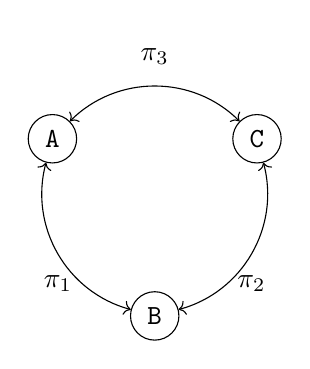
\begin{tikzpicture}[node distance=1cm, every node/.style={draw,
						circle, minimum height=0.1cm, minimum width=0.1cm}]
			\node (A) at (270-120:1.5) {$\texttt{A}$};
			\node (B) at (270:1.5) {$\texttt{B}$};
			\node (C) at (270+120:1.5) {$\texttt{C}$};

			\draw[<->, bend right=45] (A) to node[midway, draw=none, below] {$\pi_1$} (B);
			\draw[<->, bend right=45] (B) to node[midway, draw=none, below] {$\pi_2$} (C);
			\draw[<->, bend right=45] (C) to node[midway, draw=none, above] {$\pi_{3}$} (A);
		\end{tikzpicture}
	\end{center}
\end{frame}

\begin{frame}[fragile]{The Bombe}
	\begin{center}
\begin{tikzpicture}[node distance=1cm, 
  every node/.style={minimum size=0.6cm},
  round/.style={draw, circle, minimum size=0.6cm},
  box/.style={draw, rectangle, minimum width=0.8cm, minimum height=0.6cm}
]
  % Main triangle nodes
  \node[round] (A) at (150:2cm) {\texttt{A}};
  \node[round] (B) at (270:2cm) {\texttt{?}};
  \node[round] (C) at (30:2cm) {\texttt{?}};

  \node[box, rotate=172-90, fill=lightgray] (PreA) at (172:2cm) {$S^$};
  \node[box, rotate=126.5-90, fill=lightgray] (PostA) at (126.5:2cm) {$S^{-1}$};
  % Arcs between main triangle nodes
  \draw[<->, bend right=43] (PreA) to node[midway, left] {$\overline\pi_1$} (B);
  \draw[<->, bend right=50] (B) to node[midway, right] {$\overline\pi_2$} (C);
  \draw[<->, bend right=42] (C) to node[midway, above] {$\overline\pi_3$} (PostA);
    % Boxes before and after A (along the same radial line)

\end{tikzpicture}
	\end{center}
\end{frame}


\begin{frame}{The Bombe}
	\begin{center}
		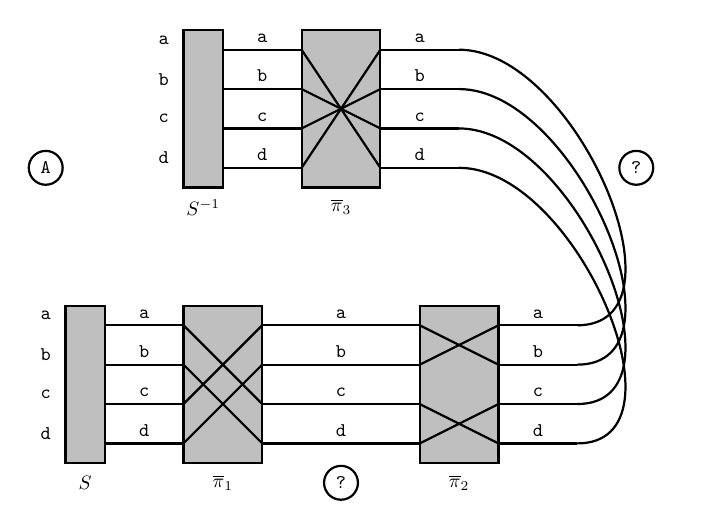
\begin{tikzpicture}[thick, scale=0.5, every node/.style={scale=0.7}]
			% Draw the box
			\draw[fill=lightgray] (2,-1.5) rectangle (4,2.5) node[midway] {};

			\node at (3, -2) {$\overline\pi_{3}$};

            \draw[fill=lightgray] (2-3,-1.5) rectangle (4-4,2.5) node[midway] {};
			\node at (3-3.5, -2) {$S^{-1}$};

            \node (Plain) at (2-3-0.5, 2+0.25) {\texttt{a}};
            \node (Plain) at (2-3-0.5, 2+0.25-1) {\texttt{b}};
            \node (Plain) at (2-3-0.5, 2+0.25-2) {\texttt{c}};
            \node (Plain) at (2-3-0.5, 2+0.25-3) {\texttt{d}};



			% Draw the wires entering the box
			\draw[-] (0, 2) -- (2, 2) node[midway, above] {\texttt{a}};
			\draw[-] (0, 1) -- (2, 1) node[midway, above] {\texttt{b}};
			\draw[-] (0, 0) -- (2, 0) node[midway, above] {\texttt{c}};
			\draw[-] (0,-1) -- (2,-1) node[midway, above] {\texttt{d}};

			% Draw the wires exiting the box with crossed mappings
			\draw[-] (4, 2) -- (6,2) node[midway, above] {\texttt{a}};
			\draw[-] (4, 1) -- (6, 1) node[midway, above] {\texttt{b}};
			\draw[-] (4, 0) -- (6, 0) node[midway, above] {\texttt{c}};
			\draw[-] (4,-1) -- (6, -1) node[midway, above] {\texttt{d}};

			% Draw the lines inside the box to represent the mapping
			\draw[-] (2, 2) -- (4,-1);
			\draw[-] (2, 1) -- (4, 0);
			\draw[-] (2, 0) -- (4, 1);
			\draw[-] (2,-1) -- (4, 2);

			\draw[-] (6+3, 2-7) to[out=360, in=360] (6, 2) node[midway, above] {};
			\draw[-] (6+3, 1-7) to[out=360, in=360] (6, 1) node[midway, above] {};
			\draw[-] (6+3, 0-7) to[out=360, in=360] (6, 0) node[midway, above] {};
			\draw[-] (6+3, -1-7) to[out=360, in=360] (6, -1) node[midway, above] {};

			\draw[fill=lightgray] (2-3,-1.5-7) rectangle (4-3,2.5-7) node[midway] {};

			\node at (3-3, -2-7) {$\overline\pi_1$};

            \draw[fill=lightgray] (2-3-3,-1.5-7) rectangle (4-4-3,2.5-7) node[midway] {};
			\node at (3-3.5-3, -2-7) {$S$};

			% Draw the wires entering the box
			\draw[-] (0-3, 2-7) -- (2-3, 2-7) node[midway, above] {\texttt{a}};
			\draw[-] (0-3, 1-7) -- (2-3, 1-7) node[midway, above] {\texttt{b}};
			\draw[-] (0-3, 0-7) -- (2-3, 0-7) node[midway, above] {\texttt{c}};
			\draw[-] (0-3,-1-7) -- (2-3,-1-7) node[midway, above] {\texttt{d}};

			% Draw the wires exiting the box
			\draw[-] (4-3, 2-7) -- (6-3,2-7) node[right, above] {\texttt{a}};
			\draw[-] (4-3, 1-7) -- (6-3, 1-7) node[right, above] {\texttt{b}};
			\draw[-] (4-3, 0-7) -- (6-3, 0-7) node[right, above] {\texttt{c}};
			\draw[-] (4-3,-1-7) -- (6-3, -1-7) node[right, above] {\texttt{d}};

			% Draw the lines inside the box to represent the mapping

			\draw[-] (2-3, 2-7) -- (4-3, 0-7);
			\draw[-] (2-3, 1-7) -- (4-3, -1-7);
			\draw[-] (2-3, 0-7) -- (4-3, 2-7);
			\draw[-] (2-3,-1-7) -- (4-3, 1-7);

            \node (Plain) at (2-3-3-0.5, 2-7+0.25) {\texttt{a}};
            \node (Plain) at (2-3-3-0.5, 2-7+0.25-1) {\texttt{b}};
            \node (Plain) at (2-3-3-0.5, 2-7+0.25-2) {\texttt{c}};
            \node (Plain) at (2-3-3-0.5, 2-7+0.25-3) {\texttt{d}};

			\draw[fill=lightgray] (2+3,-1.5-7) rectangle (4+3,2.5-7) node[midway] {};

			\node at (3+3, -2-7) {$\overline\pi_2$};

			% Draw the wires entering the box
			\draw[-] (0+3, 2-7) -- (2+3, 2-7) node[midway, above] {};
			\draw[-] (0+3, 1-7) -- (2+3, 1-7) node[midway, above] {};
			\draw[-] (0+3, 0-7) -- (2+3, 0-7) node[midway, above] {};
			\draw[-] (0+3,-1-7) -- (2+3,-1-7) node[midway, above] {};

			% Draw the wires exiting the box
			\draw[-] (4+3, 2-7) -- (6+3,2-7) node[midway, above] {\texttt{a}};
			\draw[-] (4+3, 1-7) -- (6+3, 1-7) node[midway, above] {\texttt{b}};
			\draw[-] (4+3, 0-7) -- (6+3, 0-7) node[midway, above] {\texttt{c}};
			\draw[-] (4+3,-1-7) -- (6+3, -1-7) node[midway, above] {\texttt{d}};

			\draw[-] (2+3, 2-7) -- (4+3, 1-7);
			\draw[-] (2+3, 1-7) -- (4+3, 2-7);
			\draw[-] (2+3, 0-7) -- (4+3, -1-7);
			\draw[-] (2+3,-1-7) -- (4+3, 0-7);

			\node[draw,circle] at (-4.5, -1) {\texttt{A}};
			\node[draw,circle] at (3, -9) {\texttt{?}};
			\node[draw,circle] at (10.5, -1) {\texttt{?}};

		\end{tikzpicture}.
	\end{center}
\end{frame}


\begin{frame}{The Bombe}
	\begin{center}
		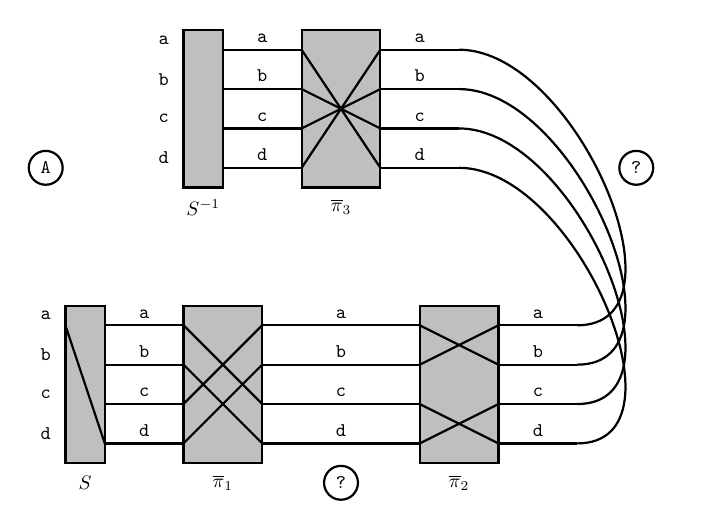
\begin{tikzpicture}[thick, scale=0.5, every node/.style={scale=0.7}]
			% Draw the box
			\draw[fill=lightgray] (2,-1.5) rectangle (4,2.5) node[midway] {};

			\node at (3, -2) {$\overline\pi_{3}$};

            \draw[fill=lightgray] (2-3,-1.5) rectangle (4-4,2.5) node[midway] {};
			\node at (3-3.5, -2) {$S^{-1}$};

            \node (Plain) at (2-3-0.5, 2+0.25) {\texttt{a}};
            \node (Plain) at (2-3-0.5, 2+0.25-1) {\texttt{b}};
            \node (Plain) at (2-3-0.5, 2+0.25-2) {\texttt{c}};
            \node (Plain) at (2-3-0.5, 2+0.25-3) {\texttt{d}};

			% Draw the wires entering the box
			\draw[-] (0, 2) -- (2, 2) node[midway, above] {\texttt{a}};
			\draw[-] (0, 1) -- (2, 1) node[midway, above] {\texttt{b}};
			\draw[-] (0, 0) -- (2, 0) node[midway, above] {\texttt{c}};
			\draw[-] (0,-1) -- (2,-1) node[midway, above] {\texttt{d}};

			% Draw the wires exiting the box with crossed mappings
			\draw[-] (4, 2) -- (6,2) node[midway, above] {\texttt{a}};
			\draw[-] (4, 1) -- (6, 1) node[midway, above] {\texttt{b}};
			\draw[-] (4, 0) -- (6, 0) node[midway, above] {\texttt{c}};
			\draw[-] (4,-1) -- (6, -1) node[midway, above] {\texttt{d}};

			% Draw the lines inside the box to represent the mapping
			\draw[-] (2, 2) -- (4,-1);
			\draw[-] (2, 1) -- (4, 0);
			\draw[-] (2, 0) -- (4, 1);
			\draw[-] (2,-1) -- (4, 2);

			% \draw[-] (0-3, 2-7) to[out=180, in=180] (0, 2) node[midway, above] {};
			% \draw[-] (0-3, 1-7) to[out=180, in=180] (0, 1) node[midway, above] {};
			% \draw[-] (0-3, 0-7) to[out=180, in=180] (0, 0) node[midway, above] {};
			% \draw[-] (0-3, -1-7) to[out=180, in=180] (0, -1) node[midway, above] {};

			\draw[-] (6+3, 2-7) to[out=360, in=360] (6, 2) node[midway, above] {};
			\draw[-] (6+3, 1-7) to[out=360, in=360] (6, 1) node[midway, above] {};
			\draw[-] (6+3, 0-7) to[out=360, in=360] (6, 0) node[midway, above] {};
			\draw[-] (6+3, -1-7) to[out=360, in=360] (6, -1) node[midway, above] {};

			\draw[fill=lightgray] (2-3,-1.5-7) rectangle (4-3,2.5-7) node[midway] {};

			\node at (3-3, -2-7) {$\overline\pi_1$};

            \draw[fill=lightgray] (2-3-3,-1.5-7) rectangle (4-4-3,2.5-7) node[midway] {};
			\node at (3-3.5-3, -2-7) {$S$};

			% Draw the wires entering the box
			\draw[-] (0-3, 2-7) -- (2-3, 2-7) node[midway, above] {\texttt{a}};
			\draw[-] (0-3, 1-7) -- (2-3, 1-7) node[midway, above] {\texttt{b}};
			\draw[-] (0-3, 0-7) -- (2-3, 0-7) node[midway, above] {\texttt{c}};
			\draw[-] (0-3,-1-7) -- (2-3,-1-7) node[midway, above] {\texttt{d}};

			% Draw the wires exiting the box
			\draw[-] (4-3, 2-7) -- (6-3,2-7) node[right, above] {\texttt{a}};
			\draw[-] (4-3, 1-7) -- (6-3, 1-7) node[right, above] {\texttt{b}};
			\draw[-] (4-3, 0-7) -- (6-3, 0-7) node[right, above] {\texttt{c}};
			\draw[-] (4-3,-1-7) -- (6-3, -1-7) node[right, above] {\texttt{d}};

			% Draw the lines inside the box to represent the mapping
            \draw[-] (2-3-3, 2-7) -- (4-3-4, -1-7);
			\draw[-] (2-3, 2-7) -- (4-3, 0-7);
			\draw[-] (2-3, 1-7) -- (4-3, -1-7);
			\draw[-] (2-3, 0-7) -- (4-3, 2-7);
			\draw[-] (2-3,-1-7) -- (4-3, 1-7);

            \node (Plain) at (2-3-3-0.5, 2-7+0.25) {\texttt{a}};
            \node (Plain) at (2-3-3-0.5, 2-7+0.25-1) {\texttt{b}};
            \node (Plain) at (2-3-3-0.5, 2-7+0.25-2) {\texttt{c}};
            \node (Plain) at (2-3-3-0.5, 2-7+0.25-3) {\texttt{d}};

			\draw[fill=lightgray] (2+3,-1.5-7) rectangle (4+3,2.5-7) node[midway] {};

			\node at (3+3, -2-7) {$\overline\pi_2$};

			% Draw the wires entering the box
			\draw[-] (0+3, 2-7) -- (2+3, 2-7) node[midway, above] {};
			\draw[-] (0+3, 1-7) -- (2+3, 1-7) node[midway, above] {};
			\draw[-] (0+3, 0-7) -- (2+3, 0-7) node[midway, above] {};
			\draw[-] (0+3,-1-7) -- (2+3,-1-7) node[midway, above] {};

			% Draw the wires exiting the box
			\draw[-] (4+3, 2-7) -- (6+3,2-7) node[midway, above] {\texttt{a}};
			\draw[-] (4+3, 1-7) -- (6+3, 1-7) node[midway, above] {\texttt{b}};
			\draw[-] (4+3, 0-7) -- (6+3, 0-7) node[midway, above] {\texttt{c}};
			\draw[-] (4+3,-1-7) -- (6+3, -1-7) node[midway, above] {\texttt{d}};

			\draw[-] (2+3, 2-7) -- (4+3, 1-7);
			\draw[-] (2+3, 1-7) -- (4+3, 2-7);
			\draw[-] (2+3, 0-7) -- (4+3, -1-7);
			\draw[-] (2+3,-1-7) -- (4+3, 0-7);

			\node[draw,circle] at (-4.5, -1) {\texttt{A}};
			\node[draw,circle] at (3, -9) {\texttt{?}};
			\node[draw,circle] at (10.5, -1) {\texttt{?}};

		\end{tikzpicture}.
	\end{center}
\end{frame}

\begin{frame}{The Bombe}
	\begin{center}
		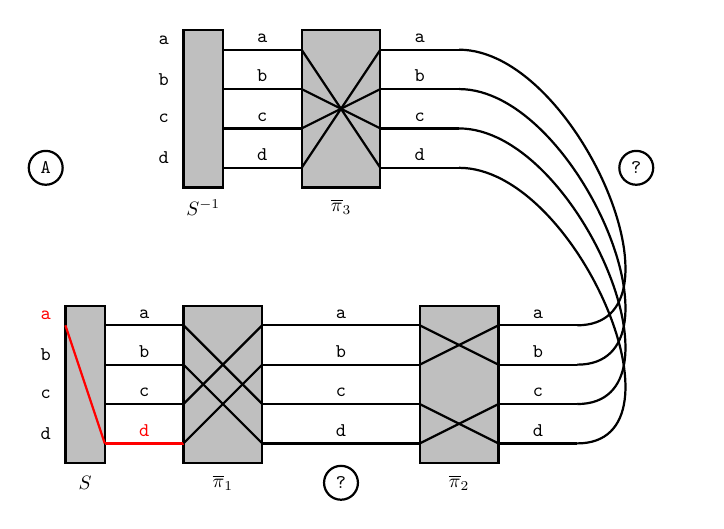
\begin{tikzpicture}[thick, scale=0.5, every node/.style={scale=0.7}]
			% Draw the box
			\draw[fill=lightgray] (2,-1.5) rectangle (4,2.5) node[midway] {};

			\node at (3, -2) {$\overline\pi_{3}$};

            \draw[fill=lightgray] (2-3,-1.5) rectangle (4-4,2.5) node[midway] {};
			\node at (3-3.5, -2) {$S^{-1}$};

            \node (Plain) at (2-3-0.5, 2+0.25) {\texttt{a}};
            \node (Plain) at (2-3-0.5, 2+0.25-1) {\texttt{b}};
            \node (Plain) at (2-3-0.5, 2+0.25-2) {\texttt{c}};
            \node (Plain) at (2-3-0.5, 2+0.25-3) {\texttt{d}};

			% Draw the wires entering the box
			\draw[-] (0, 2) -- (2, 2) node[midway, above] {\texttt{a}};
			\draw[-] (0, 1) -- (2, 1) node[midway, above] {\texttt{b}};
			\draw[-] (0, 0) -- (2, 0) node[midway, above] {\texttt{c}};
			\draw[-] (0,-1) -- (2,-1) node[midway, above] {\texttt{d}};

			% Draw the wires exiting the box with crossed mappings
			\draw[-] (4, 2) -- (6,2) node[midway, above] {\texttt{a}};
			\draw[-] (4, 1) -- (6, 1) node[midway, above] {\texttt{b}};
			\draw[-] (4, 0) -- (6, 0) node[midway, above] {\texttt{c}};
			\draw[-] (4,-1) -- (6, -1) node[midway, above] {\texttt{d}};

			% Draw the lines inside the box to represent the mapping
			\draw[-] (2, 2) -- (4,-1);
			\draw[-] (2, 1) -- (4, 0);
			\draw[-] (2, 0) -- (4, 1);
			\draw[-] (2,-1) -- (4, 2);

			% \draw[-] (0-3, 2-7) to[out=180, in=180] (0, 2) node[midway, above] {};
			% \draw[-] (0-3, 1-7) to[out=180, in=180] (0, 1) node[midway, above] {};
			% \draw[-] (0-3, 0-7) to[out=180, in=180] (0, 0) node[midway, above] {};
			% \draw[-] (0-3, -1-7) to[out=180, in=180] (0, -1) node[midway, above] {};

			\draw[-] (6+3, 2-7) to[out=360, in=360] (6, 2) node[midway, above] {};
			\draw[-] (6+3, 1-7) to[out=360, in=360] (6, 1) node[midway, above] {};
			\draw[-] (6+3, 0-7) to[out=360, in=360] (6, 0) node[midway, above] {};
			\draw[-] (6+3, -1-7) to[out=360, in=360] (6, -1) node[midway, above] {};

			\draw[fill=lightgray] (2-3,-1.5-7) rectangle (4-3,2.5-7) node[midway] {};

			\node at (3-3, -2-7) {$\overline\pi_1$};

            \draw[fill=lightgray] (2-3-3,-1.5-7) rectangle (4-4-3,2.5-7) node[midway] {};
			\node at (3-3.5-3, -2-7) {$S$};

			% Draw the wires entering the box
			\draw[-] (0-3, 2-7) -- (2-3, 2-7) node[midway, above] {\texttt{a}};
			\draw[-] (0-3, 1-7) -- (2-3, 1-7) node[midway, above] {\texttt{b}};
			\draw[-] (0-3, 0-7) -- (2-3, 0-7) node[midway, above] {\texttt{c}};
			\draw[-, red] (0-3,-1-7) -- (2-3,-1-7) node[midway, above] {\texttt{d}};

			% Draw the wires exiting the box
			\draw[-] (4-3, 2-7) -- (6-3,2-7) node[right, above] {\texttt{a}};
			\draw[-] (4-3, 1-7) -- (6-3, 1-7) node[right, above] {\texttt{b}};
			\draw[-] (4-3, 0-7) -- (6-3, 0-7) node[right, above] {\texttt{c}};
			\draw[-] (4-3,-1-7) -- (6-3, -1-7) node[right, above] {\texttt{d}};

			% Draw the lines inside the box to represent the mapping
            \draw[-, red] (2-3-3, 2-7) -- (4-3-4, -1-7);
			\draw[-] (2-3, 2-7) -- (4-3, 0-7);
			\draw[-] (2-3, 1-7) -- (4-3, -1-7);
			\draw[-] (2-3, 0-7) -- (4-3, 2-7);
			\draw[-] (2-3,-1-7) -- (4-3, 1-7);

            \node[text=red] (Plain) at (2-3-3-0.5, 2-7+0.25) {\texttt{a}};
            \node (Plain) at (2-3-3-0.5, 2-7+0.25-1) {\texttt{b}};
            \node (Plain) at (2-3-3-0.5, 2-7+0.25-2) {\texttt{c}};
            \node (Plain) at (2-3-3-0.5, 2-7+0.25-3) {\texttt{d}};

			\draw[fill=lightgray] (2+3,-1.5-7) rectangle (4+3,2.5-7) node[midway] {};

			\node at (3+3, -2-7) {$\overline\pi_2$};

			% Draw the wires entering the box
			\draw[-] (0+3, 2-7) -- (2+3, 2-7) node[midway, above] {};
			\draw[-] (0+3, 1-7) -- (2+3, 1-7) node[midway, above] {};
			\draw[-] (0+3, 0-7) -- (2+3, 0-7) node[midway, above] {};
			\draw[-] (0+3,-1-7) -- (2+3,-1-7) node[midway, above] {};

			% Draw the wires exiting the box
			\draw[-] (4+3, 2-7) -- (6+3,2-7) node[midway, above] {\texttt{a}};
			\draw[-] (4+3, 1-7) -- (6+3, 1-7) node[midway, above] {\texttt{b}};
			\draw[-] (4+3, 0-7) -- (6+3, 0-7) node[midway, above] {\texttt{c}};
			\draw[-] (4+3,-1-7) -- (6+3, -1-7) node[midway, above] {\texttt{d}};

			\draw[-] (2+3, 2-7) -- (4+3, 1-7);
			\draw[-] (2+3, 1-7) -- (4+3, 2-7);
			\draw[-] (2+3, 0-7) -- (4+3, -1-7);
			\draw[-] (2+3,-1-7) -- (4+3, 0-7);

			\node[draw,circle] at (-4.5, -1) {\texttt{A}};
			\node[draw,circle] at (3, -9) {\texttt{?}};
			\node[draw,circle] at (10.5, -1) {\texttt{?}};

		\end{tikzpicture}.
	\end{center}
\end{frame}


\begin{frame}{The Bombe}
	\begin{center}
		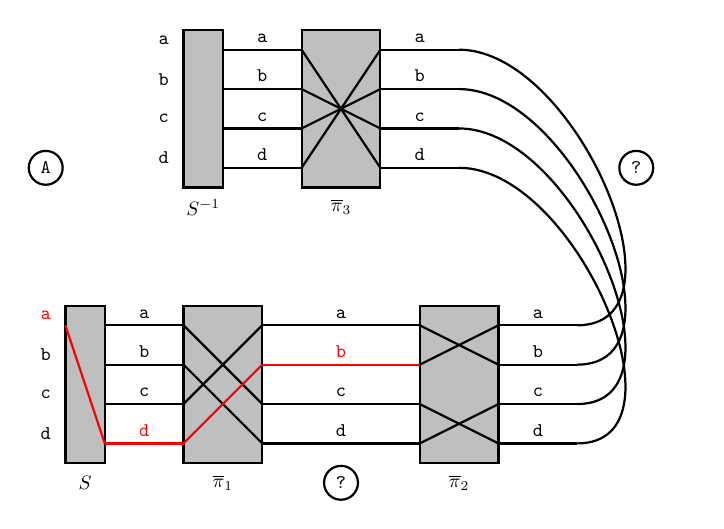
\begin{tikzpicture}[thick, scale=0.5, every node/.style={scale=0.7}]
			% Draw the box
			\draw[fill=lightgray] (2,-1.5) rectangle (4,2.5) node[midway] {};

			\node at (3, -2) {$\overline\pi_{3}$};

            \draw[fill=lightgray] (2-3,-1.5) rectangle (4-4,2.5) node[midway] {};
			\node at (3-3.5, -2) {$S^{-1}$};

            \node (Plain) at (2-3-0.5, 2+0.25) {\texttt{a}};
            \node (Plain) at (2-3-0.5, 2+0.25-1) {\texttt{b}};
            \node (Plain) at (2-3-0.5, 2+0.25-2) {\texttt{c}};
            \node (Plain) at (2-3-0.5, 2+0.25-3) {\texttt{d}};

			% Draw the wires entering the box
			\draw[-] (0, 2) -- (2, 2) node[midway, above] {\texttt{a}};
			\draw[-] (0, 1) -- (2, 1) node[midway, above] {\texttt{b}};
			\draw[-] (0, 0) -- (2, 0) node[midway, above] {\texttt{c}};
			\draw[-] (0,-1) -- (2,-1) node[midway, above] {\texttt{d}};

			% Draw the wires exiting the box with crossed mappings
			\draw[-] (4, 2) -- (6,2) node[midway, above] {\texttt{a}};
			\draw[-] (4, 1) -- (6, 1) node[midway, above] {\texttt{b}};
			\draw[-] (4, 0) -- (6, 0) node[midway, above] {\texttt{c}};
			\draw[-] (4,-1) -- (6, -1) node[midway, above] {\texttt{d}};

			% Draw the lines inside the box to represent the mapping
			\draw[-] (2, 2) -- (4,-1);
			\draw[-] (2, 1) -- (4, 0);
			\draw[-] (2, 0) -- (4, 1);
			\draw[-] (2,-1) -- (4, 2);

			% \draw[-] (0-3, 2-7) to[out=180, in=180] (0, 2) node[midway, above] {};
			% \draw[-] (0-3, 1-7) to[out=180, in=180] (0, 1) node[midway, above] {};
			% \draw[-] (0-3, 0-7) to[out=180, in=180] (0, 0) node[midway, above] {};
			% \draw[-] (0-3, -1-7) to[out=180, in=180] (0, -1) node[midway, above] {};

			\draw[-] (6+3, 2-7) to[out=360, in=360] (6, 2) node[midway, above] {};
			\draw[-] (6+3, 1-7) to[out=360, in=360] (6, 1) node[midway, above] {};
			\draw[-] (6+3, 0-7) to[out=360, in=360] (6, 0) node[midway, above] {};
			\draw[-] (6+3, -1-7) to[out=360, in=360] (6, -1) node[midway, above] {};

			\draw[fill=lightgray] (2-3,-1.5-7) rectangle (4-3,2.5-7) node[midway] {};

			\node at (3-3, -2-7) {$\overline\pi_1$};

            \draw[fill=lightgray] (2-3-3,-1.5-7) rectangle (4-4-3,2.5-7) node[midway] {};
			\node at (3-3.5-3, -2-7) {$S$};

			% Draw the wires entering the box
			\draw[-] (0-3, 2-7) -- (2-3, 2-7) node[midway, above] {\texttt{a}};
			\draw[-] (0-3, 1-7) -- (2-3, 1-7) node[midway, above] {\texttt{b}};
			\draw[-] (0-3, 0-7) -- (2-3, 0-7) node[midway, above] {\texttt{c}};
			\draw[-, red] (0-3,-1-7) -- (2-3,-1-7) node[midway, above] {\texttt{d}};

			% Draw the wires exiting the box
			\draw[-] (4-3, 2-7) -- (6-3,2-7) node[right, above] {\texttt{a}};
			\draw[-, red] (4-3, 1-7) -- (6-3, 1-7) node[right, above] {\texttt{b}};
			\draw[-] (4-3, 0-7) -- (6-3, 0-7) node[right, above] {\texttt{c}};
			\draw[-] (4-3,-1-7) -- (6-3, -1-7) node[right, above] {\texttt{d}};

			% Draw the lines inside the box to represent the mapping
            \draw[-, red] (2-3-3, 2-7) -- (4-3-4, -1-7);
			\draw[-] (2-3, 2-7) -- (4-3, 0-7);
			\draw[-] (2-3, 1-7) -- (4-3, -1-7);
			\draw[-] (2-3, 0-7) -- (4-3, 2-7);
			\draw[-, red] (2-3,-1-7) -- (4-3, 1-7);

            \node[text=red] (Plain) at (2-3-3-0.5, 2-7+0.25) {\texttt{a}};
            \node (Plain) at (2-3-3-0.5, 2-7+0.25-1) {\texttt{b}};
            \node (Plain) at (2-3-3-0.5, 2-7+0.25-2) {\texttt{c}};
            \node (Plain) at (2-3-3-0.5, 2-7+0.25-3) {\texttt{d}};

			\draw[fill=lightgray] (2+3,-1.5-7) rectangle (4+3,2.5-7) node[midway] {};

			\node at (3+3, -2-7) {$\overline\pi_2$};

			% Draw the wires entering the box
			\draw[-] (0+3, 2-7) -- (2+3, 2-7) node[midway, above] {};
			\draw[-, red] (0+3, 1-7) -- (2+3, 1-7) node[midway, above] {};
			\draw[-] (0+3, 0-7) -- (2+3, 0-7) node[midway, above] {};
			\draw[-] (0+3,-1-7) -- (2+3,-1-7) node[midway, above] {};

			% Draw the wires exiting the box
			\draw[-] (4+3, 2-7) -- (6+3,2-7) node[midway, above] {\texttt{a}};
			\draw[-] (4+3, 1-7) -- (6+3, 1-7) node[midway, above] {\texttt{b}};
			\draw[-] (4+3, 0-7) -- (6+3, 0-7) node[midway, above] {\texttt{c}};
			\draw[-] (4+3,-1-7) -- (6+3, -1-7) node[midway, above] {\texttt{d}};

			\draw[-] (2+3, 2-7) -- (4+3, 1-7);
			\draw[-] (2+3, 1-7) -- (4+3, 2-7);
			\draw[-] (2+3, 0-7) -- (4+3, -1-7);
			\draw[-] (2+3,-1-7) -- (4+3, 0-7);

			\node[draw,circle] at (-4.5, -1) {\texttt{A}};
			\node[draw,circle] at (3, -9) {\texttt{?}};
			\node[draw,circle] at (10.5, -1) {\texttt{?}};

		\end{tikzpicture}.
	\end{center}
\end{frame}

\begin{frame}{The Bombe}
	\begin{center}
		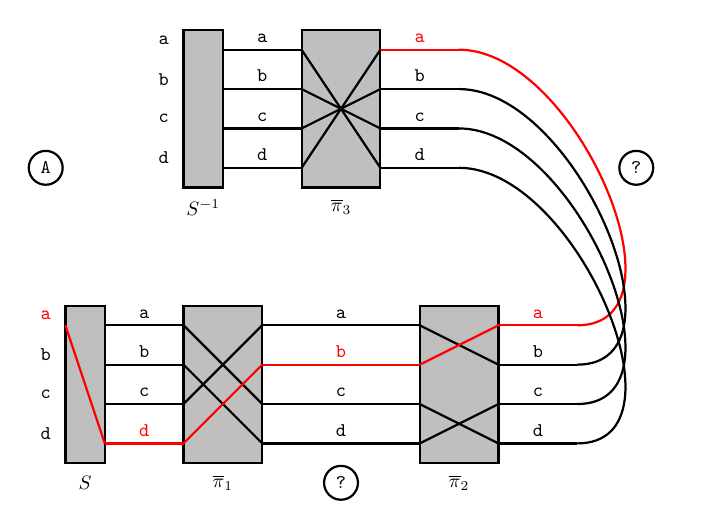
\begin{tikzpicture}[thick, scale=0.5, every node/.style={scale=0.7}]
			% Draw the box
			\draw[fill=lightgray] (2,-1.5) rectangle (4,2.5) node[midway] {};

			\node at (3, -2) {$\overline\pi_{3}$};

            \draw[fill=lightgray] (2-3,-1.5) rectangle (4-4,2.5) node[midway] {};
			\node at (3-3.5, -2) {$S^{-1}$};

            \node (Plain) at (2-3-0.5, 2+0.25) {\texttt{a}};
            \node (Plain) at (2-3-0.5, 2+0.25-1) {\texttt{b}};
            \node (Plain) at (2-3-0.5, 2+0.25-2) {\texttt{c}};
            \node (Plain) at (2-3-0.5, 2+0.25-3) {\texttt{d}};

			% Draw the wires entering the box
			\draw[-] (0, 2) -- (2, 2) node[midway, above] {\texttt{a}};
			\draw[-] (0, 1) -- (2, 1) node[midway, above] {\texttt{b}};
			\draw[-] (0, 0) -- (2, 0) node[midway, above] {\texttt{c}};
			\draw[-] (0,-1) -- (2,-1) node[midway, above] {\texttt{d}};

			% Draw the wires exiting the box with crossed mappings
			\draw[-, red] (4, 2) -- (6,2) node[midway, above] {\texttt{a}};
			\draw[-] (4, 1) -- (6, 1) node[midway, above] {\texttt{b}};
			\draw[-] (4, 0) -- (6, 0) node[midway, above] {\texttt{c}};
			\draw[-] (4,-1) -- (6, -1) node[midway, above] {\texttt{d}};

			% Draw the lines inside the box to represent the mapping
			\draw[-] (2, 2) -- (4,-1);
			\draw[-] (2, 1) -- (4, 0);
			\draw[-] (2, 0) -- (4, 1);
			\draw[-] (2,-1) -- (4, 2);

			% \draw[-] (0-3, 2-7) to[out=180, in=180] (0, 2) node[midway, above] {};
			% \draw[-] (0-3, 1-7) to[out=180, in=180] (0, 1) node[midway, above] {};
			% \draw[-] (0-3, 0-7) to[out=180, in=180] (0, 0) node[midway, above] {};
			% \draw[-] (0-3, -1-7) to[out=180, in=180] (0, -1) node[midway, above] {};

			\draw[-, red] (6+3, 2-7) to[out=360, in=360] (6, 2) node[midway, above] {};
			\draw[-] (6+3, 1-7) to[out=360, in=360] (6, 1) node[midway, above] {};
			\draw[-] (6+3, 0-7) to[out=360, in=360] (6, 0) node[midway, above] {};
			\draw[-] (6+3, -1-7) to[out=360, in=360] (6, -1) node[midway, above] {};

			\draw[fill=lightgray] (2-3,-1.5-7) rectangle (4-3,2.5-7) node[midway] {};

			\node at (3-3, -2-7) {$\overline\pi_1$};

            \draw[fill=lightgray] (2-3-3,-1.5-7) rectangle (4-4-3,2.5-7) node[midway] {};
			\node at (3-3.5-3, -2-7) {$S$};

			% Draw the wires entering the box
			\draw[-] (0-3, 2-7) -- (2-3, 2-7) node[midway, above] {\texttt{a}};
			\draw[-] (0-3, 1-7) -- (2-3, 1-7) node[midway, above] {\texttt{b}};
			\draw[-] (0-3, 0-7) -- (2-3, 0-7) node[midway, above] {\texttt{c}};
			\draw[-, red] (0-3,-1-7) -- (2-3,-1-7) node[midway, above] {\texttt{d}};

			% Draw the wires exiting the box
			\draw[-] (4-3, 2-7) -- (6-3,2-7) node[right, above] {\texttt{a}};
			\draw[-, red] (4-3, 1-7) -- (6-3, 1-7) node[right, above] {\texttt{b}};
			\draw[-] (4-3, 0-7) -- (6-3, 0-7) node[right, above] {\texttt{c}};
			\draw[-] (4-3,-1-7) -- (6-3, -1-7) node[right, above] {\texttt{d}};

			% Draw the lines inside the box to represent the mapping
            \draw[-, red] (2-3-3, 2-7) -- (4-3-4, -1-7);
			\draw[-] (2-3, 2-7) -- (4-3, 0-7);
			\draw[-] (2-3, 1-7) -- (4-3, -1-7);
			\draw[-] (2-3, 0-7) -- (4-3, 2-7);
			\draw[-, red] (2-3,-1-7) -- (4-3, 1-7);

            \node[text=red] (Plain) at (2-3-3-0.5, 2-7+0.25) {\texttt{a}};
            \node (Plain) at (2-3-3-0.5, 2-7+0.25-1) {\texttt{b}};
            \node (Plain) at (2-3-3-0.5, 2-7+0.25-2) {\texttt{c}};
            \node (Plain) at (2-3-3-0.5, 2-7+0.25-3) {\texttt{d}};

			\draw[fill=lightgray] (2+3,-1.5-7) rectangle (4+3,2.5-7) node[midway] {};

			\node at (3+3, -2-7) {$\overline\pi_2$};

			% Draw the wires entering the box
			\draw[-] (0+3, 2-7) -- (2+3, 2-7) node[midway, above] {};
			\draw[-, red] (0+3, 1-7) -- (2+3, 1-7) node[midway, above] {};
			\draw[-] (0+3, 0-7) -- (2+3, 0-7) node[midway, above] {};
			\draw[-] (0+3,-1-7) -- (2+3,-1-7) node[midway, above] {};

			% Draw the wires exiting the box
			\draw[-, red] (4+3, 2-7) -- (6+3,2-7) node[midway, above] {\texttt{a}};
			\draw[-] (4+3, 1-7) -- (6+3, 1-7) node[midway, above] {\texttt{b}};
			\draw[-] (4+3, 0-7) -- (6+3, 0-7) node[midway, above] {\texttt{c}};
			\draw[-] (4+3,-1-7) -- (6+3, -1-7) node[midway, above] {\texttt{d}};

			\draw[-] (2+3, 2-7) -- (4+3, 1-7);
			\draw[-, red] (2+3, 1-7) -- (4+3, 2-7);
			\draw[-] (2+3, 0-7) -- (4+3, -1-7);
			\draw[-] (2+3,-1-7) -- (4+3, 0-7);

			\node[draw,circle] at (-4.5, -1) {\texttt{A}};
			\node[draw,circle] at (3, -9) {\texttt{?}};
			\node[draw,circle] at (10.5, -1) {\texttt{?}};

		\end{tikzpicture}.
	\end{center}
\end{frame}

\begin{frame}{The Bombe}
	\begin{center}
		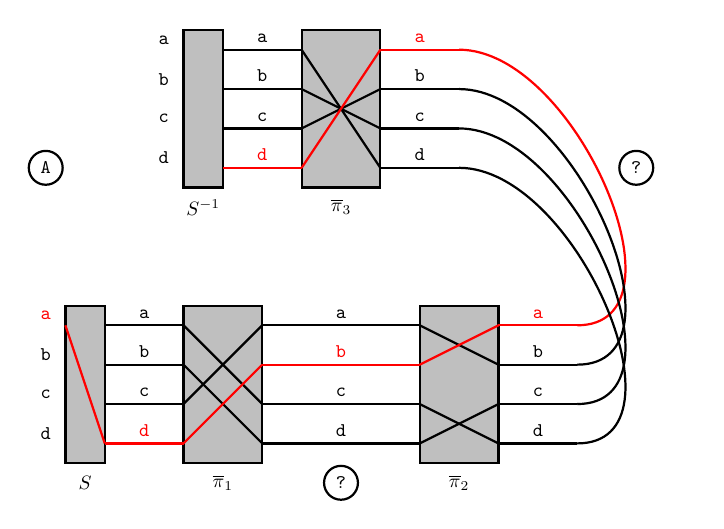
\begin{tikzpicture}[thick, scale=0.5, every node/.style={scale=0.7}]
			% Draw the box
			\draw[fill=lightgray] (2,-1.5) rectangle (4,2.5) node[midway] {};

			\node at (3, -2) {$\overline\pi_{3}$};

            \draw[fill=lightgray] (2-3,-1.5) rectangle (4-4,2.5) node[midway] {};
			\node at (3-3.5, -2) {$S^{-1}$};

            \node (Plain) at (2-3-0.5, 2+0.25) {\texttt{a}};
            \node (Plain) at (2-3-0.5, 2+0.25-1) {\texttt{b}};
            \node (Plain) at (2-3-0.5, 2+0.25-2) {\texttt{c}};
            \node (Plain) at (2-3-0.5, 2+0.25-3) {\texttt{d}};

			% Draw the wires entering the box
			\draw[-] (0, 2) -- (2, 2) node[midway, above] {\texttt{a}};
			\draw[-] (0, 1) -- (2, 1) node[midway, above] {\texttt{b}};
			\draw[-] (0, 0) -- (2, 0) node[midway, above] {\texttt{c}};
			\draw[-, red] (0,-1) -- (2,-1) node[midway, above] {\texttt{d}};

			% Draw the wires exiting the box with crossed mappings
			\draw[-, red] (4, 2) -- (6,2) node[midway, above] {\texttt{a}};
			\draw[-] (4, 1) -- (6, 1) node[midway, above] {\texttt{b}};
			\draw[-] (4, 0) -- (6, 0) node[midway, above] {\texttt{c}};
			\draw[-] (4,-1) -- (6, -1) node[midway, above] {\texttt{d}};

			% Draw the lines inside the box to represent the mapping
			\draw[-] (2, 2) -- (4,-1);
			\draw[-] (2, 1) -- (4, 0);
			\draw[-] (2, 0) -- (4, 1);
			\draw[-, red] (2,-1) -- (4, 2);

			% \draw[-] (0-3, 2-7) to[out=180, in=180] (0, 2) node[midway, above] {};
			% \draw[-] (0-3, 1-7) to[out=180, in=180] (0, 1) node[midway, above] {};
			% \draw[-] (0-3, 0-7) to[out=180, in=180] (0, 0) node[midway, above] {};
			% \draw[-] (0-3, -1-7) to[out=180, in=180] (0, -1) node[midway, above] {};

			\draw[-, red] (6+3, 2-7) to[out=360, in=360] (6, 2) node[midway, above] {};
			\draw[-] (6+3, 1-7) to[out=360, in=360] (6, 1) node[midway, above] {};
			\draw[-] (6+3, 0-7) to[out=360, in=360] (6, 0) node[midway, above] {};
			\draw[-] (6+3, -1-7) to[out=360, in=360] (6, -1) node[midway, above] {};

			\draw[fill=lightgray] (2-3,-1.5-7) rectangle (4-3,2.5-7) node[midway] {};

			\node at (3-3, -2-7) {$\overline\pi_1$};

            \draw[fill=lightgray] (2-3-3,-1.5-7) rectangle (4-4-3,2.5-7) node[midway] {};
			\node at (3-3.5-3, -2-7) {$S$};

			% Draw the wires entering the box
			\draw[-] (0-3, 2-7) -- (2-3, 2-7) node[midway, above] {\texttt{a}};
			\draw[-] (0-3, 1-7) -- (2-3, 1-7) node[midway, above] {\texttt{b}};
			\draw[-] (0-3, 0-7) -- (2-3, 0-7) node[midway, above] {\texttt{c}};
			\draw[-, red] (0-3,-1-7) -- (2-3,-1-7) node[midway, above] {\texttt{d}};

			% Draw the wires exiting the box
			\draw[-] (4-3, 2-7) -- (6-3,2-7) node[right, above] {\texttt{a}};
			\draw[-, red] (4-3, 1-7) -- (6-3, 1-7) node[right, above] {\texttt{b}};
			\draw[-] (4-3, 0-7) -- (6-3, 0-7) node[right, above] {\texttt{c}};
			\draw[-] (4-3,-1-7) -- (6-3, -1-7) node[right, above] {\texttt{d}};

			% Draw the lines inside the box to represent the mapping
            \draw[-, red] (2-3-3, 2-7) -- (4-3-4, -1-7);
			\draw[-] (2-3, 2-7) -- (4-3, 0-7);
			\draw[-] (2-3, 1-7) -- (4-3, -1-7);
			\draw[-] (2-3, 0-7) -- (4-3, 2-7);
			\draw[-, red] (2-3,-1-7) -- (4-3, 1-7);

            \node[text=red] (Plain) at (2-3-3-0.5, 2-7+0.25) {\texttt{a}};
            \node (Plain) at (2-3-3-0.5, 2-7+0.25-1) {\texttt{b}};
            \node (Plain) at (2-3-3-0.5, 2-7+0.25-2) {\texttt{c}};
            \node (Plain) at (2-3-3-0.5, 2-7+0.25-3) {\texttt{d}};

			\draw[fill=lightgray] (2+3,-1.5-7) rectangle (4+3,2.5-7) node[midway] {};

			\node at (3+3, -2-7) {$\overline\pi_2$};

			% Draw the wires entering the box
			\draw[-] (0+3, 2-7) -- (2+3, 2-7) node[midway, above] {};
			\draw[-, red] (0+3, 1-7) -- (2+3, 1-7) node[midway, above] {};
			\draw[-] (0+3, 0-7) -- (2+3, 0-7) node[midway, above] {};
			\draw[-] (0+3,-1-7) -- (2+3,-1-7) node[midway, above] {};

			% Draw the wires exiting the box
			\draw[-, red] (4+3, 2-7) -- (6+3,2-7) node[midway, above] {\texttt{a}};
			\draw[-] (4+3, 1-7) -- (6+3, 1-7) node[midway, above] {\texttt{b}};
			\draw[-] (4+3, 0-7) -- (6+3, 0-7) node[midway, above] {\texttt{c}};
			\draw[-] (4+3,-1-7) -- (6+3, -1-7) node[midway, above] {\texttt{d}};

			\draw[-] (2+3, 2-7) -- (4+3, 1-7);
			\draw[-, red] (2+3, 1-7) -- (4+3, 2-7);
			\draw[-] (2+3, 0-7) -- (4+3, -1-7);
			\draw[-] (2+3,-1-7) -- (4+3, 0-7);

			\node[draw,circle] at (-4.5, -1) {\texttt{A}};
			\node[draw,circle] at (3, -9) {\texttt{?}};
			\node[draw,circle] at (10.5, -1) {\texttt{?}};

		\end{tikzpicture}.
	\end{center}
\end{frame}

\begin{frame}{The Bombe}
	\begin{center}
		\begin{tikzpicture}[thick, scale=0.5, every node/.style={scale=0.7}]
			% Draw the box
			\draw[fill=lightgray] (2,-1.5) rectangle (4,2.5) node[midway] {};

			\node at (3, -2) {$\overline\pi_{3}$};

            \draw[fill=lightgray] (2-3,-1.5) rectangle (4-4,2.5) node[midway] {};
			\node at (3-3.5, -2) {$S^{-1}$};

            \node[text=red] (Plain) at (2-3-0.5, 2+0.25) {\texttt{a}};
            \node (Plain) at (2-3-0.5, 2+0.25-1) {\texttt{b}};
            \node (Plain) at (2-3-0.5, 2+0.25-2) {\texttt{c}};
            \node (Plain) at (2-3-0.5, 2+0.25-3) {\texttt{d}};

			% Draw the wires entering the box
			\draw[-] (0, 2) -- (2, 2) node[midway, above] {\texttt{a}};
			\draw[-] (0, 1) -- (2, 1) node[midway, above] {\texttt{b}};
			\draw[-] (0, 0) -- (2, 0) node[midway, above] {\texttt{c}};
			\draw[-, red] (0,-1) -- (2,-1) node[midway, above] {\texttt{d}};
            \draw[-, red] (2-3,2) -- (3-3,-1) node[midway, above];

			% Draw the wires exiting the box with crossed mappings
			\draw[-, red] (4, 2) -- (6,2) node[midway, above] {\texttt{a}};
			\draw[-] (4, 1) -- (6, 1) node[midway, above] {\texttt{b}};
			\draw[-] (4, 0) -- (6, 0) node[midway, above] {\texttt{c}};
			\draw[-] (4,-1) -- (6, -1) node[midway, above] {\texttt{d}};

			% Draw the lines inside the box to represent the mapping
			\draw[-] (2, 2) -- (4,-1);
			\draw[-] (2, 1) -- (4, 0);
			\draw[-] (2, 0) -- (4, 1);
			\draw[-, red] (2,-1) -- (4, 2);

			% \draw[-] (0-3, 2-7) to[out=180, in=180] (0, 2) node[midway, above] {};
			% \draw[-] (0-3, 1-7) to[out=180, in=180] (0, 1) node[midway, above] {};
			% \draw[-] (0-3, 0-7) to[out=180, in=180] (0, 0) node[midway, above] {};
			% \draw[-] (0-3, -1-7) to[out=180, in=180] (0, -1) node[midway, above] {};

			\draw[-, red] (6+3, 2-7) to[out=360, in=360] (6, 2) node[midway, above] {};
			\draw[-] (6+3, 1-7) to[out=360, in=360] (6, 1) node[midway, above] {};
			\draw[-] (6+3, 0-7) to[out=360, in=360] (6, 0) node[midway, above] {};
			\draw[-] (6+3, -1-7) to[out=360, in=360] (6, -1) node[midway, above] {};

			\draw[fill=lightgray] (2-3,-1.5-7) rectangle (4-3,2.5-7) node[midway] {};

			\node at (3-3, -2-7) {$\overline\pi_1$};

            \draw[fill=lightgray] (2-3-3,-1.5-7) rectangle (4-4-3,2.5-7) node[midway] {};
			\node at (3-3.5-3, -2-7) {$S$};

			% Draw the wires entering the box
			\draw[-] (0-3, 2-7) -- (2-3, 2-7) node[midway, above] {\texttt{a}};
			\draw[-] (0-3, 1-7) -- (2-3, 1-7) node[midway, above] {\texttt{b}};
			\draw[-] (0-3, 0-7) -- (2-3, 0-7) node[midway, above] {\texttt{c}};
			\draw[-, red] (0-3,-1-7) -- (2-3,-1-7) node[midway, above] {\texttt{d}};

			% Draw the wires exiting the box
			\draw[-] (4-3, 2-7) -- (6-3,2-7) node[right, above] {\texttt{a}};
			\draw[-, red] (4-3, 1-7) -- (6-3, 1-7) node[right, above] {\texttt{b}};
			\draw[-] (4-3, 0-7) -- (6-3, 0-7) node[right, above] {\texttt{c}};
			\draw[-] (4-3,-1-7) -- (6-3, -1-7) node[right, above] {\texttt{d}};

			% Draw the lines inside the box to represent the mapping
            \draw[-, red] (2-3-3, 2-7) -- (4-3-4, -1-7);
			\draw[-] (2-3, 2-7) -- (4-3, 0-7);
			\draw[-] (2-3, 1-7) -- (4-3, -1-7);
			\draw[-] (2-3, 0-7) -- (4-3, 2-7);
			\draw[-, red] (2-3,-1-7) -- (4-3, 1-7);

            \node[text=red] (Plain) at (2-3-3-0.5, 2-7+0.25) {\texttt{a}};
            \node (Plain) at (2-3-3-0.5, 2-7+0.25-1) {\texttt{b}};
            \node (Plain) at (2-3-3-0.5, 2-7+0.25-2) {\texttt{c}};
            \node (Plain) at (2-3-3-0.5, 2-7+0.25-3) {\texttt{d}};

			\draw[fill=lightgray] (2+3,-1.5-7) rectangle (4+3,2.5-7) node[midway] {};

			\node at (3+3, -2-7) {$\overline\pi_2$};

			% Draw the wires entering the box
			\draw[-] (0+3, 2-7) -- (2+3, 2-7) node[midway, above] {};
			\draw[-, red] (0+3, 1-7) -- (2+3, 1-7) node[midway, above] {};
			\draw[-] (0+3, 0-7) -- (2+3, 0-7) node[midway, above] {};
			\draw[-] (0+3,-1-7) -- (2+3,-1-7) node[midway, above] {};

			% Draw the wires exiting the box
			\draw[-, red] (4+3, 2-7) -- (6+3,2-7) node[midway, above] {\texttt{a}};
			\draw[-] (4+3, 1-7) -- (6+3, 1-7) node[midway, above] {\texttt{b}};
			\draw[-] (4+3, 0-7) -- (6+3, 0-7) node[midway, above] {\texttt{c}};
			\draw[-] (4+3,-1-7) -- (6+3, -1-7) node[midway, above] {\texttt{d}};

			\draw[-] (2+3, 2-7) -- (4+3, 1-7);
			\draw[-, red] (2+3, 1-7) -- (4+3, 2-7);
			\draw[-] (2+3, 0-7) -- (4+3, -1-7);
			\draw[-] (2+3,-1-7) -- (4+3, 0-7);

			\node[draw,circle] at (-4.5, -1) {\texttt{A}};
			\node[draw,circle] at (3, -9) {\texttt{?}};
			\node[draw,circle] at (10.5, -1) {\texttt{?}};

		\end{tikzpicture}.
	\end{center}
\end{frame}

\begin{frame}{The Bombe}
    \begin{center}
    For a different set of $\overline\pi_i$...
    \end{center}
	\begin{center}
		\begin{tikzpicture}[thick, scale=0.42, every node/.style={scale=0.7}]
			% Draw the box
			\draw[fill=lightgray] (2,-1.5) rectangle (4,2.5) node[midway] {};

			\node at (3, -2) {$\overline\pi_{3}$};

            \draw[fill=lightgray] (2-3,-1.5) rectangle (4-4,2.5) node[midway] {};
			\node at (3-3.5, -2) {$S^{-1}$};

            \node[text=red] (Plain) at (2-3-0.5, 2+0.25) {\texttt{a}};
            \node (Plain) at (2-3-0.5, 2+0.25-1) {\texttt{b}};
            \node (Plain) at (2-3-0.5, 2+0.25-2) {\texttt{c}};
            \node (Plain) at (2-3-0.5, 2+0.25-3) {\texttt{d}};

			% Draw the wires entering the box
			\draw[-, red] (0, 2) -- (2, 2) node[midway, above] {\texttt{a}};
			\draw[-] (0, 1) -- (2, 1) node[midway, above] {\texttt{b}};
			\draw[-] (0, 0) -- (2, 0) node[midway, above] {\texttt{c}};
			\draw[-] (0,-1) -- (2,-1) node[midway, above] {\texttt{d}};
            \draw[-, red] (2-3,2) -- (3-3,2) node[midway, above];

			% Draw the wires exiting the box with crossed mappings
			\draw[-] (4, 2) -- (6,2) node[midway, above] {\texttt{a}};
			\draw[-] (4, 1) -- (6, 1) node[midway, above] {\texttt{b}};
			\draw[-] (4, 0) -- (6, 0) node[midway, above] {\texttt{c}};
			\draw[-, red] (4,-1) -- (6, -1) node[midway, above] {\texttt{d}};

			% Draw the lines inside the box to represent the mapping
			\draw[-, red] (2, 2) -- (4,-1);
			\draw[-] (2, 1) -- (4, 0);
			\draw[-] (2, 0) -- (4, 1);
			\draw[-] (2,-1) -- (4, 2);

			% \draw[-] (0-3, 2-7) to[out=180, in=180] (0, 2) node[midway, above] {};
			% \draw[-] (0-3, 1-7) to[out=180, in=180] (0, 1) node[midway, above] {};
			% \draw[-] (0-3, 0-7) to[out=180, in=180] (0, 0) node[midway, above] {};
			% \draw[-] (0-3, -1-7) to[out=180, in=180] (0, -1) node[midway, above] {};

			\draw[-] (6+3, 2-7) to[out=360, in=360] (6, 2) node[midway, above] {};
			\draw[-] (6+3, 1-7) to[out=360, in=360] (6, 1) node[midway, above] {};
			\draw[-] (6+3, 0-7) to[out=360, in=360] (6, 0) node[midway, above] {};
			\draw[-, red] (6+3, -1-7) to[out=360, in=360] (6, -1) node[midway, above] {};

			\draw[fill=lightgray] (2-3,-1.5-7) rectangle (4-3,2.5-7) node[midway] {};

			\node at (3-3, -2-7) {$\overline\pi_1$};

            \draw[fill=lightgray] (2-3-3,-1.5-7) rectangle (4-4-3,2.5-7) node[midway] {};
			\node at (3-3.5-3, -2-7) {$S$};

			% Draw the wires entering the box
			\draw[-] (0-3, 2-7) -- (2-3, 2-7) node[midway, above] {\texttt{a}};
			\draw[-] (0-3, 1-7) -- (2-3, 1-7) node[midway, above] {\texttt{b}};
			\draw[-] (0-3, 0-7) -- (2-3, 0-7) node[midway, above] {\texttt{c}};
			\draw[-, red] (0-3,-1-7) -- (2-3,-1-7) node[midway, above] {\texttt{d}};

			% Draw the wires exiting the box
			\draw[-] (4-3, 2-7) -- (6-3,2-7) node[right, above] {\texttt{a}};
			\draw[-, red] (4-3, 1-7) -- (6-3, 1-7) node[right, above] {\texttt{b}};
			\draw[-] (4-3, 0-7) -- (6-3, 0-7) node[right, above] {\texttt{c}};
			\draw[-] (4-3,-1-7) -- (6-3, -1-7) node[right, above] {\texttt{d}};

			% Draw the lines inside the box to represent the mapping
            \draw[-, red] (2-3-3, 2-7) -- (4-3-4, -1-7);
			\draw[-] (2-3, 2-7) -- (4-3, 0-7);
			\draw[-] (2-3, 1-7) -- (4-3, -1-7);
			\draw[-] (2-3, 0-7) -- (4-3, 2-7);
			\draw[-, red] (2-3,-1-7) -- (4-3, 1-7);

            \node[text=red] (Plain) at (2-3-3-0.5, 2-7+0.25) {\texttt{a}};
            \node (Plain) at (2-3-3-0.5, 2-7+0.25-1) {\texttt{b}};
            \node (Plain) at (2-3-3-0.5, 2-7+0.25-2) {\texttt{c}};
            \node (Plain) at (2-3-3-0.5, 2-7+0.25-3) {\texttt{d}};

			\draw[fill=lightgray] (2+3,-1.5-7) rectangle (4+3,2.5-7) node[midway] {};

			\node at (3+3, -2-7) {$\overline\pi_2$};

			% Draw the wires entering the box
			\draw[-] (0+3, 2-7) -- (2+3, 2-7) node[midway, above] {};
			\draw[-, red] (0+3, 1-7) -- (2+3, 1-7) node[midway, above] {};
			\draw[-] (0+3, 0-7) -- (2+3, 0-7) node[midway, above] {};
			\draw[-] (0+3,-1-7) -- (2+3,-1-7) node[midway, above] {};

			% Draw the wires exiting the box
			\draw[-] (4+3, 2-7) -- (6+3,2-7) node[midway, above] {\texttt{a}};
			\draw[-] (4+3, 1-7) -- (6+3, 1-7) node[midway, above] {\texttt{b}};
			\draw[-] (4+3, 0-7) -- (6+3, 0-7) node[midway, above] {\texttt{c}};
			\draw[-, red] (4+3,-1-7) -- (6+3, -1-7) node[midway, above] {\texttt{d}};

			\draw[-] (2+3, 2-7) -- (4+3, 0-7);
			\draw[-,red] (2+3, 1-7) -- (4+3, -1-7);
			\draw[-] (2+3, 0-7) -- (4+3, 2-7);
			\draw[-] (2+3,-1-7) -- (4+3, 1-7);

			\node[draw,circle] at (-4.5, -1) {\texttt{A}};
			\node[draw,circle] at (3, -9) {\texttt{?}};
			\node[draw,circle] at (10.5, -1) {\texttt{?}};

		\end{tikzpicture}.
	\end{center}
    \begin{center}
        a contradiction!
    \end{center}
\end{frame}

% \begin{frame}{The Bombe}
% 	\begin{center}
% 		\begin{tikzpicture}[thick, scale=0.5, every node/.style={scale=0.7}]
% 			% Draw the box
% 			\draw[fill=lightgray] (2,-1.5) rectangle (4,2.5) node[midway] {};

% 			\node at (3, -2) {$\overline\pi_{3}$};


% 			% Draw the wires entering the box
% 			\draw[-] (0, 2) -- (2, 2) node[midway, above] {\texttt{a}};
% 			\draw[-] (0, 1) -- (2, 1) node[midway, above] {\texttt{b}};
% 			\draw[-] (0, 0) -- (2, 0) node[midway, above] {\texttt{c}};
% 			\draw[-] (0,-1) -- (2,-1) node[midway, above] {\texttt{d}};

% 			% Draw the wires exiting the box with crossed mappings
% 			\draw[-] (4, 2) -- (6,2) node[midway, above] {\texttt{a}};
% 			\draw[-] (4, 1) -- (6, 1) node[midway, above] {\texttt{b}};
% 			\draw[-] (4, 0) -- (6, 0) node[midway, above] {\texttt{c}};
% 			\draw[-] (4,-1) -- (6, -1) node[midway, above] {\texttt{d}};

% 			% Draw the lines inside the box to represent the mapping
% 			\draw[-] (2, 2) -- (4,-1);
% 			\draw[-] (2, 1) -- (4, 0);
% 			\draw[-] (2, 0) -- (4, 1);
% 			\draw[-] (2,-1) -- (4, 2);

% 			% \draw[-] (0-3, 2-7) to[out=180, in=180] (0, 2) node[midway, above] {};
% 			% \draw[-] (0-3, 1-7) to[out=180, in=180] (0, 1) node[midway, above] {};
% 			% \draw[-] (0-3, 0-7) to[out=180, in=180] (0, 0) node[midway, above] {};
% 			% \draw[-] (0-3, -1-7) to[out=180, in=180] (0, -1) node[midway, above] {};

% 			\draw[-] (6+3, 2-7) to[out=360, in=360] (6, 2) node[midway, above] {};
% 			\draw[-] (6+3, 1-7) to[out=360, in=360] (6, 1) node[midway, above] {};
% 			\draw[-] (6+3, 0-7) to[out=360, in=360] (6, 0) node[midway, above] {};
% 			\draw[-] (6+3, -1-7) to[out=360, in=360] (6, -1) node[midway, above] {};

% 			\draw[fill=lightgray] (2-3,-1.5-7) rectangle (4-3,2.5-7) node[midway] {};

% 			\node at (3-3, -2-7) {$\overline\pi_1$};

% 			% Draw the wires entering the box
% 			\draw[-] (0-3, 2-7) -- (2-3, 2-7) node[midway, above] {\texttt{a}};
% 			\draw[-] (0-3, 1-7) -- (2-3, 1-7) node[midway, above] {\texttt{b}};
% 			\draw[-] (0-3, 0-7) -- (2-3, 0-7) node[midway, above] {\texttt{c}};
% 			\draw[-] (0-3,-1-7) -- (2-3,-1-7) node[midway, above] {\texttt{d}};

% 			% Draw the wires exiting the box
% 			\draw[-] (4-3, 2-7) -- (6-3,2-7) node[right, above] {\texttt{a}};
% 			\draw[-] (4-3, 1-7) -- (6-3, 1-7) node[right, above] {\texttt{b}};
% 			\draw[-] (4-3, 0-7) -- (6-3, 0-7) node[right, above] {\texttt{c}};
% 			\draw[-] (4-3,-1-7) -- (6-3, -1-7) node[right, above] {\texttt{d}};

% 			% Draw the lines inside the box to represent the mapping
% 			\draw[-] (2-3, 2-7) -- (4-3, 0-7);
% 			\draw[-] (2-3, 1-7) -- (4-3, -1-7);
% 			\draw[-] (2-3, 0-7) -- (4-3, 2-7);
% 			\draw[-] (2-3,-1-7) -- (4-3, 1-7);

% 			\draw[fill=lightgray] (2+3,-1.5-7) rectangle (4+3,2.5-7) node[midway] {};

% 			\node at (3+3, -2-7) {$\overline\pi_2$};

% 			% Draw the wires entering the box
% 			\draw[-] (0+3, 2-7) -- (2+3, 2-7) node[midway, above] {};
% 			\draw[-] (0+3, 1-7) -- (2+3, 1-7) node[midway, above] {};
% 			\draw[-] (0+3, 0-7) -- (2+3, 0-7) node[midway, above] {};
% 			\draw[-] (0+3,-1-7) -- (2+3,-1-7) node[midway, above] {};

% 			% Draw the wires exiting the box
% 			\draw[-] (4+3, 2-7) -- (6+3,2-7) node[midway, above] {\texttt{a}};
% 			\draw[-] (4+3, 1-7) -- (6+3, 1-7) node[midway, above] {\texttt{b}};
% 			\draw[-] (4+3, 0-7) -- (6+3, 0-7) node[midway, above] {\texttt{c}};
% 			\draw[-] (4+3,-1-7) -- (6+3, -1-7) node[midway, above] {\texttt{d}};

% 			\draw[-] (2+3, 2-7) -- (4+3, 1-7);
% 			\draw[-] (2+3, 1-7) -- (4+3, 2-7);
% 			\draw[-] (2+3, 0-7) -- (4+3, -1-7);
% 			\draw[-] (2+3,-1-7) -- (4+3, 0-7);

% 			\node[draw,circle] at (-4.5, -1) {\texttt{A}};
% 			\node[draw,circle] at (3, -9) {\texttt{B}};
% 			\node[draw,circle] at (10.5, -1) {\texttt{C}};

% 		\end{tikzpicture}.
% 	\end{center}
% \end{frame}


% \begin{frame}{The Bombe}
% 	\begin{center}
% 		\begin{tikzpicture}[thick, scale=0.5, every node/.style={scale=0.7}]
% 			% Draw the box
% 			\draw[fill=lightgray] (2,-1.5) rectangle (4,2.5) node[midway] {};

% 			\node at (3, -2) {$\overline\pi_{3}$};

% 			% Draw the wires entering the box
% 			\draw[-] (0, 2) -- (2, 2) node[midway, above] {\texttt{a}};
% 			\draw[-] (0, 1) -- (2, 1) node[midway, above] {\texttt{b}};
% 			\draw[-] (0, 0) -- (2, 0) node[midway, above] {\texttt{c}};
% 			\draw[-, red] (0,-1) -- (2,-1) node[midway, above] {\texttt{d}};

% 			% Draw the wires exiting the box with crossed mappings
% 			\draw[-] (4, 2) -- (6,2) node[midway, above] {\texttt{a}};
% 			\draw[-] (4, 1) -- (6, 1) node[midway, above] {\texttt{b}};
% 			\draw[-] (4, 0) -- (6, 0) node[midway, above] {\texttt{c}};
% 			\draw[-] (4,-1) -- (6, -1) node[midway, above] {\texttt{d}};

% 			% Draw the lines inside the box to represent the mapping
% 			\draw[-] (2, 2) -- (4,-1);
% 			\draw[-] (2, 1) -- (4, 0);
% 			\draw[-] (2, 0) -- (4, 1);
% 			\draw[-] (2,-1) -- (4, 2);

% 			\draw[-] (0-3, 2-7) to[out=180, in=180] (0, 2) node[midway, above] {};
% 			\draw[-] (0-3, 1-7) to[out=180, in=180] (0, 1) node[midway, above] {};
% 			\draw[-] (0-3, 0-7) to[out=180, in=180] (0, 0) node[midway, above] {};
% 			\draw[-, red] (0-3, -1-7) to[out=180, in=180] (0, -1) node[midway, above] {};

% 			\draw[-] (6+3, 2-7) to[out=360, in=360] (6, 2) node[midway, above] {};
% 			\draw[-] (6+3, 1-7) to[out=360, in=360] (6, 1) node[midway, above] {};
% 			\draw[-] (6+3, 0-7) to[out=360, in=360] (6, 0) node[midway, above] {};
% 			\draw[-] (6+3, -1-7) to[out=360, in=360] (6, -1) node[midway, above] {};

% 			\draw[fill=lightgray] (2-3,-1.5-7) rectangle (4-3,2.5-7) node[midway] {};

% 			\node at (3-3, -2-7) {$\overline\pi_1$};

% 			% Draw the wires entering the box
% 			\draw[-] (0-3, 2-7) -- (2-3, 2-7) node[midway, above] {\texttt{a}};
% 			\draw[-] (0-3, 1-7) -- (2-3, 1-7) node[midway, above] {\texttt{b}};
% 			\draw[-] (0-3, 0-7) -- (2-3, 0-7) node[midway, above] {\texttt{c}};
% 			\draw[-, red] (0-3,-1-7) -- (2-3,-1-7) node[midway, above] {\texttt{d}};

% 			% Draw the wires exiting the box
% 			\draw[-] (4-3, 2-7) -- (6-3,2-7) node[right, above] {\texttt{a}};
% 			\draw[-] (4-3, 1-7) -- (6-3, 1-7) node[right, above] {\texttt{b}};
% 			\draw[-] (4-3, 0-7) -- (6-3, 0-7) node[right, above] {\texttt{c}};
% 			\draw[-] (4-3,-1-7) -- (6-3, -1-7) node[right, above] {\texttt{d}};

% 			% Draw the lines inside the box to represent the mapping
% 			\draw[-] (2-3, 2-7) -- (4-3, 0-7);
% 			\draw[-] (2-3, 1-7) -- (4-3, -1-7);
% 			\draw[-] (2-3, 0-7) -- (4-3, 2-7);
% 			\draw[-] (2-3,-1-7) -- (4-3, 1-7);

% 			\draw[fill=lightgray] (2+3,-1.5-7) rectangle (4+3,2.5-7) node[midway] {};

% 			\node at (3+3, -2-7) {$\overline\pi_2$};

% 			% Draw the wires entering the box
% 			\draw[-] (0+3, 2-7) -- (2+3, 2-7) node[midway, above] {};
% 			\draw[-] (0+3, 1-7) -- (2+3, 1-7) node[midway, above] {};
% 			\draw[-] (0+3, 0-7) -- (2+3, 0-7) node[midway, above] {};
% 			\draw[-] (0+3,-1-7) -- (2+3,-1-7) node[midway, above] {};

% 			% Draw the wires exiting the box
% 			\draw[-] (4+3, 2-7) -- (6+3,2-7) node[midway, above] {\texttt{a}};
% 			\draw[-] (4+3, 1-7) -- (6+3, 1-7) node[midway, above] {\texttt{b}};
% 			\draw[-] (4+3, 0-7) -- (6+3, 0-7) node[midway, above] {\texttt{c}};
% 			\draw[-] (4+3,-1-7) -- (6+3, -1-7) node[midway, above] {\texttt{d}};

% 			\draw[-] (2+3, 2-7) -- (4+3, 1-7);
% 			\draw[-] (2+3, 1-7) -- (4+3, 2-7);
% 			\draw[-] (2+3, 0-7) -- (4+3, -1-7);
% 			\draw[-] (2+3,-1-7) -- (4+3, 0-7);

% 			\node[draw,circle] at (-4.5, -1) {\texttt{A}};
% 			\node[draw,circle] at (3, -9) {\texttt{B}};
% 			\node[draw,circle] at (10.5, -1) {\texttt{C}};

% 		\end{tikzpicture}.
% 	\end{center}
% \end{frame}


% \begin{frame}{The Bombe}
% 	\begin{center}
% 		\begin{tikzpicture}[thick, scale=0.5, every node/.style={scale=0.7}]
% 			% Draw the box
% 			\draw[fill=lightgray] (2,-1.5) rectangle (4,2.5) node[midway] {};

% 			\node at (3, -2) {$\overline\pi_{3}$};

% 			% Draw the wires entering the box
% 			\draw[-] (0, 2) -- (2, 2) node[midway, above] {\texttt{a}};
% 			\draw[-] (0, 1) -- (2, 1) node[midway, above] {\texttt{b}};
% 			\draw[-] (0, 0) -- (2, 0) node[midway, above] {\texttt{c}};
% 			\draw[-, red] (0,-1) -- (2,-1) node[midway, above] {\texttt{d}};

% 			% Draw the wires exiting the box with crossed mappings
% 			\draw[-] (4, 2) -- (6,2) node[midway, above] {\texttt{a}};
% 			\draw[-] (4, 1) -- (6, 1) node[midway, above] {\texttt{b}};
% 			\draw[-] (4, 0) -- (6, 0) node[midway, above] {\texttt{c}};
% 			\draw[-] (4,-1) -- (6, -1) node[midway, above] {\texttt{d}};

% 			% Draw the lines inside the box to represent the mapping
% 			\draw[-] (2, 2) -- (4,-1);
% 			\draw[-] (2, 1) -- (4, 0);
% 			\draw[-] (2, 0) -- (4, 1);
% 			\draw[-] (2,-1) -- (4, 2);

% 			\draw[-] (0-3, 2-7) to[out=180, in=180] (0, 2) node[midway, above] {};
% 			\draw[-] (0-3, 1-7) to[out=180, in=180] (0, 1) node[midway, above] {};
% 			\draw[-] (0-3, 0-7) to[out=180, in=180] (0, 0) node[midway, above] {};
% 			\draw[-, red] (0-3, -1-7) to[out=180, in=180] (0, -1) node[midway, above] {};

% 			\draw[-] (6+3, 2-7) to[out=360, in=360] (6, 2) node[midway, above] {};
% 			\draw[-] (6+3, 1-7) to[out=360, in=360] (6, 1) node[midway, above] {};
% 			\draw[-] (6+3, 0-7) to[out=360, in=360] (6, 0) node[midway, above] {};
% 			\draw[-] (6+3, -1-7) to[out=360, in=360] (6, -1) node[midway, above] {};

% 			\draw[fill=lightgray] (2-3,-1.5-7) rectangle (4-3,2.5-7) node[midway] {};

% 			\node at (3-3, -2-7) {$\overline\pi_1$};

% 			% Draw the wires entering the box
% 			\draw[-] (0-3, 2-7) -- (2-3, 2-7) node[midway, above] {\texttt{a}};
% 			\draw[-] (0-3, 1-7) -- (2-3, 1-7) node[midway, above] {\texttt{b}};
% 			\draw[-] (0-3, 0-7) -- (2-3, 0-7) node[midway, above] {\texttt{c}};
% 			\draw[-, red] (0-3,-1-7) -- (2-3,-1-7) node[midway, above] {\texttt{d}};

% 			% Draw the wires exiting the box
% 			\draw[-] (4-3, 2-7) -- (6-3,2-7) node[right, above] {\texttt{a}};
% 			\draw[-, red] (4-3, 1-7) -- (6-3, 1-7) node[right, above] {\texttt{b}};
% 			\draw[-] (4-3, 0-7) -- (6-3, 0-7) node[right, above] {\texttt{c}};
% 			\draw[-] (4-3,-1-7) -- (6-3, -1-7) node[right, above] {\texttt{d}};

% 			% Draw the lines inside the box to represent the mapping
% 			\draw[-] (2-3, 2-7) -- (4-3, 0-7);
% 			\draw[-] (2-3, 1-7) -- (4-3, -1-7);
% 			\draw[-] (2-3, 0-7) -- (4-3, 2-7);
% 			\draw[-, red] (2-3,-1-7) -- (4-3, 1-7);

% 			\draw[fill=lightgray] (2+3,-1.5-7) rectangle (4+3,2.5-7) node[midway] {};

% 			\node at (3+3, -2-7) {$\overline\pi_2$};

% 			% Draw the wires entering the box
% 			\draw[-] (0+3, 2-7) -- (2+3, 2-7) node[midway, above] {};
% 			\draw[-, red] (0+3, 1-7) -- (2+3, 1-7) node[midway, above] {};
% 			\draw[-] (0+3, 0-7) -- (2+3, 0-7) node[midway, above] {};
% 			\draw[-] (0+3,-1-7) -- (2+3,-1-7) node[midway, above] {};

% 			% Draw the wires exiting the box
% 			\draw[-] (4+3, 2-7) -- (6+3,2-7) node[midway, above] {\texttt{a}};
% 			\draw[-] (4+3, 1-7) -- (6+3, 1-7) node[midway, above] {\texttt{b}};
% 			\draw[-] (4+3, 0-7) -- (6+3, 0-7) node[midway, above] {\texttt{c}};
% 			\draw[-] (4+3,-1-7) -- (6+3, -1-7) node[midway, above] {\texttt{d}};

% 			\draw[-] (2+3, 2-7) -- (4+3, 1-7);
% 			\draw[-] (2+3, 1-7) -- (4+3, 2-7);
% 			\draw[-] (2+3, 0-7) -- (4+3, -1-7);
% 			\draw[-] (2+3,-1-7) -- (4+3, 0-7);

% 			\node[draw,circle] at (-4.5, -1) {\texttt{A}};
% 			\node[draw,circle] at (3, -9) {\texttt{B}};
% 			\node[draw,circle] at (10.5, -1) {\texttt{C}};

% 		\end{tikzpicture}.
% 	\end{center}
% \end{frame}

% \begin{frame}{The Bombe}
% 	\begin{center}
% 		\begin{tikzpicture}[thick, scale=0.5, every node/.style={scale=0.7}]
% 			% Draw the box
% 			\draw[fill=lightgray] (2,-1.5) rectangle (4,2.5) node[midway] {};

% 			\node at (3, -2) {$\overline\pi_{3}$};

% 			% Draw the wires entering the box
% 			\draw[-] (0, 2) -- (2, 2) node[midway, above] {\texttt{a}};
% 			\draw[-] (0, 1) -- (2, 1) node[midway, above] {\texttt{b}};
% 			\draw[-] (0, 0) -- (2, 0) node[midway, above] {\texttt{c}};
% 			\draw[-, red] (0,-1) -- (2,-1) node[midway, above] {\texttt{d}};

% 			% Draw the wires exiting the box with crossed mappings
% 			\draw[-, red] (4, 2) -- (6,2) node[midway, above] {\texttt{a}};
% 			\draw[-] (4, 1) -- (6, 1) node[midway, above] {\texttt{b}};
% 			\draw[-] (4, 0) -- (6, 0) node[midway, above] {\texttt{c}};
% 			\draw[-] (4,-1) -- (6, -1) node[midway, above] {\texttt{d}};

% 			% Draw the lines inside the box to represent the mapping
% 			\draw[-] (2, 2) -- (4,-1);
% 			\draw[-] (2, 1) -- (4, 0);
% 			\draw[-] (2, 0) -- (4, 1);
% 			\draw[-] (2,-1) -- (4, 2);

% 			\draw[-] (0-3, 2-7) to[out=180, in=180] (0, 2) node[midway, above] {};
% 			\draw[-] (0-3, 1-7) to[out=180, in=180] (0, 1) node[midway, above] {};
% 			\draw[-] (0-3, 0-7) to[out=180, in=180] (0, 0) node[midway, above] {};
% 			\draw[-, red] (0-3, -1-7) to[out=180, in=180] (0, -1) node[midway, above] {};

% 			\draw[-, red] (6+3, 2-7) to[out=360, in=360] (6, 2) node[midway, above] {};
% 			\draw[-] (6+3, 1-7) to[out=360, in=360] (6, 1) node[midway, above] {};
% 			\draw[-] (6+3, 0-7) to[out=360, in=360] (6, 0) node[midway, above] {};
% 			\draw[-] (6+3, -1-7) to[out=360, in=360] (6, -1) node[midway, above] {};

% 			\draw[fill=lightgray] (2-3,-1.5-7) rectangle (4-3,2.5-7) node[midway] {};

% 			\node at (3-3, -2-7) {$\overline\pi_1$};

% 			% Draw the wires entering the box
% 			\draw[-] (0-3, 2-7) -- (2-3, 2-7) node[midway, above] {\texttt{a}};
% 			\draw[-] (0-3, 1-7) -- (2-3, 1-7) node[midway, above] {\texttt{b}};
% 			\draw[-] (0-3, 0-7) -- (2-3, 0-7) node[midway, above] {\texttt{c}};
% 			\draw[-, red] (0-3,-1-7) -- (2-3,-1-7) node[midway, above] {\texttt{d}};

% 			% Draw the wires exiting the box
% 			\draw[-] (4-3, 2-7) -- (6-3,2-7) node[right, above] {\texttt{a}};
% 			\draw[-, red] (4-3, 1-7) -- (6-3, 1-7) node[right, above] {\texttt{b}};
% 			\draw[-] (4-3, 0-7) -- (6-3, 0-7) node[right, above] {\texttt{c}};
% 			\draw[-] (4-3,-1-7) -- (6-3, -1-7) node[right, above] {\texttt{d}};

% 			% Draw the lines inside the box to represent the mapping
% 			\draw[-] (2-3, 2-7) -- (4-3, 0-7);
% 			\draw[-] (2-3, 1-7) -- (4-3, -1-7);
% 			\draw[-] (2-3, 0-7) -- (4-3, 2-7);
% 			\draw[-, red] (2-3,-1-7) -- (4-3, 1-7);

% 			\draw[fill=lightgray] (2+3,-1.5-7) rectangle (4+3,2.5-7) node[midway] {};

% 			\node at (3+3, -2-7) {$\overline\pi_2$};

% 			% Draw the wires entering the box
% 			\draw[-] (0+3, 2-7) -- (2+3, 2-7) node[midway, above] {};
% 			\draw[-, red] (0+3, 1-7) -- (2+3, 1-7) node[midway, above] {};
% 			\draw[-] (0+3, 0-7) -- (2+3, 0-7) node[midway, above] {};
% 			\draw[-] (0+3,-1-7) -- (2+3,-1-7) node[midway, above] {};

% 			% Draw the wires exiting the box
% 			\draw[-, red] (4+3, 2-7) -- (6+3,2-7) node[midway, above] {\texttt{a}};
% 			\draw[-] (4+3, 1-7) -- (6+3, 1-7) node[midway, above] {\texttt{b}};
% 			\draw[-] (4+3, 0-7) -- (6+3, 0-7) node[midway, above] {\texttt{c}};
% 			\draw[-] (4+3,-1-7) -- (6+3, -1-7) node[midway, above] {\texttt{d}};

% 			\draw[-] (2+3, 2-7) -- (4+3, 1-7);
% 			\draw[-, red] (2+3, 1-7) -- (4+3, 2-7);
% 			\draw[-] (2+3, 0-7) -- (4+3, -1-7);
% 			\draw[-] (2+3,-1-7) -- (4+3, 0-7);

% 			\node[draw,circle] at (-4.5, -1) {\texttt{A}};
% 			\node[draw,circle] at (3, -9) {\texttt{B}};
% 			\node[draw,circle] at (10.5, -1) {\texttt{C}};

% 		\end{tikzpicture}.
% 	\end{center}
% \end{frame}

% \begin{frame}{The Bombe}
% 	\begin{center}
% 		\begin{tikzpicture}[thick, scale=0.5, every node/.style={scale=0.7}]
% 			% Draw the box
% 			\draw[fill=lightgray] (2,-1.5) rectangle (4,2.5) node[midway] {};

% 			\node at (3, -2) {$\overline\pi_{3}$};

% 			% Draw the wires entering the box
% 			\draw[-] (0, 2) -- (2, 2) node[midway, above] {\texttt{a}};
% 			\draw[-] (0, 1) -- (2, 1) node[midway, above] {\texttt{b}};
% 			\draw[-] (0, 0) -- (2, 0) node[midway, above] {\texttt{c}};
% 			\draw[-, red] (0,-1) -- (2,-1) node[midway, above] {\texttt{d}};

% 			% Draw the wires exiting the box with crossed mappings
% 			\draw[-, red] (4, 2) -- (6,2) node[midway, above] {\texttt{a}};
% 			\draw[-] (4, 1) -- (6, 1) node[midway, above] {\texttt{b}};
% 			\draw[-] (4, 0) -- (6, 0) node[midway, above] {\texttt{c}};
% 			\draw[-] (4,-1) -- (6, -1) node[midway, above] {\texttt{d}};

% 			% Draw the lines inside the box to represent the mapping
% 			\draw[-] (2, 2) -- (4,-1);
% 			\draw[-] (2, 1) -- (4, 0);
% 			\draw[-] (2, 0) -- (4, 1);
% 			\draw[-, red] (2,-1) -- (4, 2);

% 			\draw[-] (0-3, 2-7) to[out=180, in=180] (0, 2) node[midway, above] {};
% 			\draw[-] (0-3, 1-7) to[out=180, in=180] (0, 1) node[midway, above] {};
% 			\draw[-] (0-3, 0-7) to[out=180, in=180] (0, 0) node[midway, above] {};
% 			\draw[-, red] (0-3, -1-7) to[out=180, in=180] (0, -1) node[midway, above] {};

% 			\draw[-, red] (6+3, 2-7) to[out=360, in=360] (6, 2) node[midway, above] {};
% 			\draw[-] (6+3, 1-7) to[out=360, in=360] (6, 1) node[midway, above] {};
% 			\draw[-] (6+3, 0-7) to[out=360, in=360] (6, 0) node[midway, above] {};
% 			\draw[-] (6+3, -1-7) to[out=360, in=360] (6, -1) node[midway, above] {};

% 			\draw[fill=lightgray] (2-3,-1.5-7) rectangle (4-3,2.5-7) node[midway] {};

% 			\node at (3-3, -2-7) {$\overline\pi_1$};

% 			% Draw the wires entering the box
% 			\draw[-] (0-3, 2-7) -- (2-3, 2-7) node[midway, above] {\texttt{a}};
% 			\draw[-] (0-3, 1-7) -- (2-3, 1-7) node[midway, above] {\texttt{b}};
% 			\draw[-] (0-3, 0-7) -- (2-3, 0-7) node[midway, above] {\texttt{c}};
% 			\draw[-, red] (0-3,-1-7) -- (2-3,-1-7) node[midway, above] {\texttt{d}};

% 			% Draw the wires exiting the box
% 			\draw[-] (4-3, 2-7) -- (6-3,2-7) node[right, above] {\texttt{a}};
% 			\draw[-, red] (4-3, 1-7) -- (6-3, 1-7) node[right, above] {\texttt{b}};
% 			\draw[-] (4-3, 0-7) -- (6-3, 0-7) node[right, above] {\texttt{c}};
% 			\draw[-] (4-3,-1-7) -- (6-3, -1-7) node[right, above] {\texttt{d}};

% 			% Draw the lines inside the box to represent the mapping
% 			\draw[-] (2-3, 2-7) -- (4-3, 0-7);
% 			\draw[-] (2-3, 1-7) -- (4-3, -1-7);
% 			\draw[-] (2-3, 0-7) -- (4-3, 2-7);
% 			\draw[-, red] (2-3,-1-7) -- (4-3, 1-7);

% 			\draw[fill=lightgray] (2+3,-1.5-7) rectangle (4+3,2.5-7) node[midway] {};

% 			\node at (3+3, -2-7) {$\overline\pi_2$};

% 			% Draw the wires entering the box
% 			\draw[-] (0+3, 2-7) -- (2+3, 2-7) node[midway, above] {};
% 			\draw[-, red] (0+3, 1-7) -- (2+3, 1-7) node[midway, above] {};
% 			\draw[-] (0+3, 0-7) -- (2+3, 0-7) node[midway, above] {};
% 			\draw[-] (0+3,-1-7) -- (2+3,-1-7) node[midway, above] {};

% 			% Draw the wires exiting the box
% 			\draw[-, red] (4+3, 2-7) -- (6+3,2-7) node[midway, above] {\texttt{a}};
% 			\draw[-] (4+3, 1-7) -- (6+3, 1-7) node[midway, above] {\texttt{b}};
% 			\draw[-] (4+3, 0-7) -- (6+3, 0-7) node[midway, above] {\texttt{c}};
% 			\draw[-] (4+3,-1-7) -- (6+3, -1-7) node[midway, above] {\texttt{d}};

% 			\draw[-] (2+3, 2-7) -- (4+3, 1-7);
% 			\draw[-, red] (2+3, 1-7) -- (4+3, 2-7);
% 			\draw[-] (2+3, 0-7) -- (4+3, -1-7);
% 			\draw[-] (2+3,-1-7) -- (4+3, 0-7);

% 			\node[draw,circle] at (-4.5, -1) {\texttt{A}};
% 			\node[draw,circle] at (3, -9) {\texttt{B}};
% 			\node[draw,circle] at (10.5, -1) {\texttt{C}};

% 		\end{tikzpicture}.
% 	\end{center}
% \end{frame}

\begin{frame}
	\begin{center}
		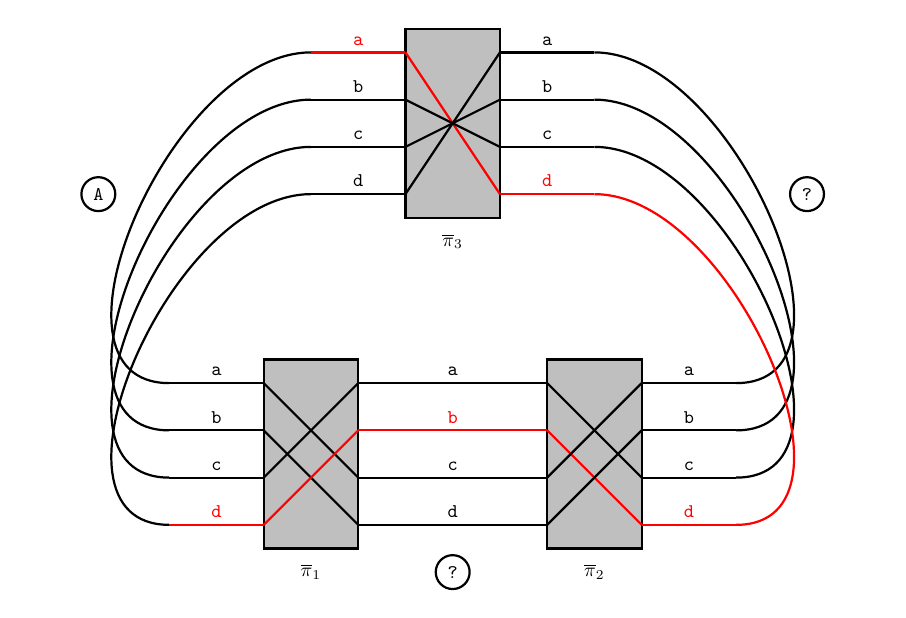
\begin{tikzpicture}[thick, scale=0.6, every node/.style={scale=0.7}]
			% Draw the box
			\draw[fill=lightgray] (2,-1.5) rectangle (4,2.5) node[midway] {};

			\node at (3, -2) {$\overline\pi_3$};

			% Draw the wires entering the box
			\draw[-, red] (0, 2) -- (2, 2) node[midway, above] {\texttt{a}};
			\draw[-] (0, 1) -- (2, 1) node[midway, above] {\texttt{b}};
			\draw[-] (0, 0) -- (2, 0) node[midway, above] {\texttt{c}};
			\draw[-] (0,-1) -- (2,-1) node[midway, above] {\texttt{d}};

			% Draw the wires exiting the box with crossed mappings
			\draw[-] (4, 2) -- (6,2) node[midway, above] {\texttt{a}};
			\draw[-] (4, 1) -- (6, 1) node[midway, above] {\texttt{b}};
			\draw[-] (4, 0) -- (6, 0) node[midway, above] {\texttt{c}};
			\draw[-, red] (4,-1) -- (6, -1) node[midway, above] {\texttt{d}};

			% Draw the lines inside the box to represent the mapping
			\draw[-, red] (2, 2) -- (4,-1);
			\draw[-] (2, 1) -- (4, 0);
			\draw[-] (2, 0) -- (4, 1);
			\draw[-] (2,-1) -- (4, 2);

			\draw[-] (0-3, 2-7) to[out=180, in=180] (0, 2) node[midway, above] {};
			\draw[-] (0-3, 1-7) to[out=180, in=180] (0, 1) node[midway, above] {};
			\draw[-] (0-3, 0-7) to[out=180, in=180] (0, 0) node[midway, above] {};
			\draw[-] (0-3, -1-7) to[out=180, in=180] (0, -1)
			node[midway, above] {};

			\draw[-] (6+3, 2-7) to[out=360, in=360] (6, 2) node[midway, above] {};
			\draw[-] (6+3, 1-7) to[out=360, in=360] (6, 1) node[midway, above] {};
			\draw[-] (6+3, 0-7) to[out=360, in=360] (6, 0) node[midway, above] {};
			\draw[-, red] (6+3, -1-7) to[out=360, in=360] (6, -1)
			node[midway, above] {};

			\draw[fill=lightgray] (2-3,-1.5-7) rectangle (4-3,2.5-7) node[midway] {};

			\node at (3-3, -2-7) {$\overline\pi_1$};

			% Draw the wires entering the box
			\draw[-] (0-3, 2-7) -- (2-3, 2-7) node[midway, above] {\texttt{a}};
			\draw[-] (0-3, 1-7) -- (2-3, 1-7) node[midway, above] {\texttt{b}};
			\draw[-] (0-3, 0-7) -- (2-3, 0-7) node[midway, above] {\texttt{c}};
			\draw[-, red] (0-3,-1-7) -- (2-3,-1-7) node[midway, above] {\texttt{d}};

			% Draw the wires exiting the box
			\draw[-] (4-3, 2-7) -- (6-3,2-7) node[right, above] {\texttt{a}};
			\draw[-, red] (4-3, 1-7) -- (6-3, 1-7) node[right, above] {\texttt{b}};
			\draw[-] (4-3, 0-7) -- (6-3, 0-7) node[right, above] {\texttt{c}};
			\draw[-] (4-3,-1-7) -- (6-3, -1-7) node[right, above] {\texttt{d}};

			% Draw the lines inside the box to represent the mapping
			\draw[-] (2-3, 2-7) -- (4-3, 0-7);
			\draw[-] (2-3, 1-7) -- (4-3, -1-7);
			\draw[-] (2-3, 0-7) -- (4-3, 2-7);
			\draw[-, red] (2-3,-1-7) -- (4-3, 1-7);

			\draw[fill=lightgray] (2+3,-1.5-7) rectangle (4+3,2.5-7) node[midway] {};

			\node at (3+3, -2-7) {$\overline\pi_2$};

			% Draw the wires entering the box
			\draw[-] (0+3, 2-7) -- (2+3, 2-7) node[midway, above] {};
			\draw[-, red] (0+3, 1-7) -- (2+3, 1-7) node[midway, above] {};
			\draw[-] (0+3, 0-7) -- (2+3, 0-7) node[midway, above] {};
			\draw[-] (0+3,-1-7) -- (2+3,-1-7) node[midway, above] {};

			% Draw the wires exiting the box
			\draw[-] (4+3, 2-7) -- (6+3,2-7) node[midway, above] {\texttt{a}};
			\draw[-] (4+3, 1-7) -- (6+3, 1-7) node[midway, above] {\texttt{b}};
			\draw[-] (4+3, 0-7) -- (6+3, 0-7) node[midway, above] {\texttt{c}};
			\draw[-, red] (4+3,-1-7) -- (6+3, -1-7) node[midway, above] {\texttt{d}};

			\draw[-] (2+3, 2-7) -- (4+3, 0-7);
			\draw[-, red] (2+3, 1-7) -- (4+3, -1-7);
			\draw[-] (2+3, 0-7) -- (4+3, 2-7);
			\draw[-] (2+3,-1-7) -- (4+3, 1-7);

			\node[draw,circle] at (-4.5, -1) {\texttt{A}};
			\node[draw,circle] at (3, -9) {\texttt{?}};
			\node[draw,circle] at (10.5, -1) {\texttt{?}};

		\end{tikzpicture}.
	\end{center}
\end{frame}

\begin{frame}
	\begin{center}
		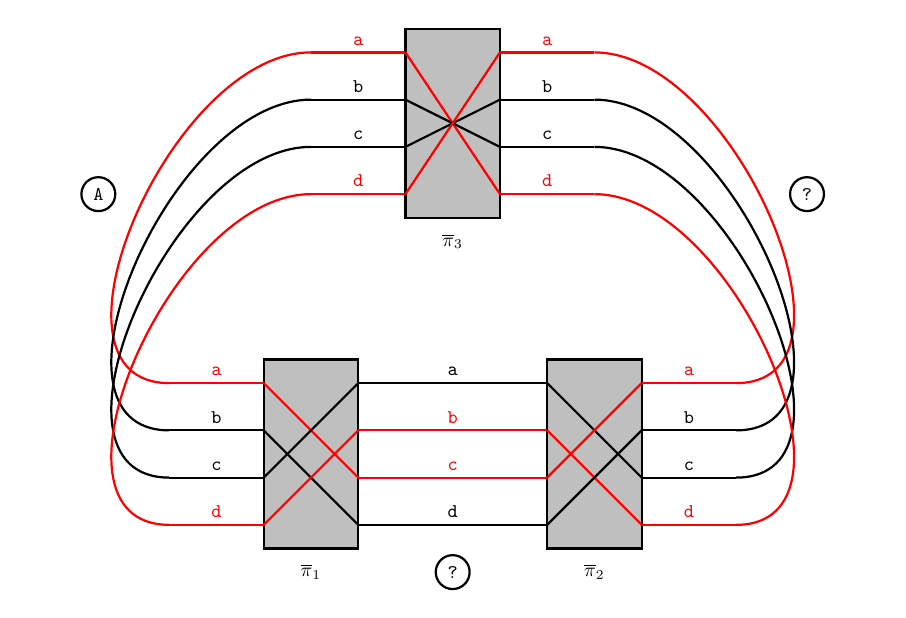
\begin{tikzpicture}[thick, scale=0.6, every node/.style={scale=0.7}]
			% Draw the box
			\draw[fill=lightgray] (2,-1.5) rectangle (4,2.5) node[midway] {};

			\node at (3, -2) {$\overline\pi_3$};

			% Draw the wires entering the box
			\draw[-, red] (0, 2) -- (2, 2) node[midway, above] {\texttt{a}};
			\draw[-] (0, 1) -- (2, 1) node[midway, above] {\texttt{b}};
			\draw[-] (0, 0) -- (2, 0) node[midway, above] {\texttt{c}};
			\draw[-, red] (0,-1) -- (2,-1) node[midway, above] {\texttt{d}};

			% Draw the wires exiting the box with crossed mappings
			\draw[-, red] (4, 2) -- (6,2) node[midway, above] {\texttt{a}};
			\draw[-] (4, 1) -- (6, 1) node[midway, above] {\texttt{b}};
			\draw[-] (4, 0) -- (6, 0) node[midway, above] {\texttt{c}};
			\draw[-, red] (4,-1) -- (6, -1) node[midway, above] {\texttt{d}};

			% Draw the lines inside the box to represent the mapping
			\draw[-, red] (2, 2) -- (4,-1);
			\draw[-] (2, 1) -- (4, 0);
			\draw[-] (2, 0) -- (4, 1);
			\draw[-, red] (2,-1) -- (4, 2);

			\draw[-, red] (0-3, 2-7) to[out=180, in=180] (0, 2) node[midway, above] {};
			\draw[-] (0-3, 1-7) to[out=180, in=180] (0, 1) node[midway, above] {};
			\draw[-] (0-3, 0-7) to[out=180, in=180] (0, 0) node[midway, above] {};
			\draw[-, red] (0-3, -1-7) to[out=180, in=180] (0, -1)
			node[midway, above] {};

			\draw[-, red] (6+3, 2-7) to[out=360, in=360] (6, 2) node[midway, above] {};
			\draw[-] (6+3, 1-7) to[out=360, in=360] (6, 1) node[midway, above] {};
			\draw[-] (6+3, 0-7) to[out=360, in=360] (6, 0) node[midway, above] {};
			\draw[-, red] (6+3, -1-7) to[out=360, in=360] (6, -1)
			node[midway, above] {};

			\draw[fill=lightgray] (2-3,-1.5-7) rectangle (4-3,2.5-7) node[midway] {};

			\node at (3-3, -2-7) {$\overline\pi_1$};

			% Draw the wires entering the box
			\draw[-, red] (0-3, 2-7) -- (2-3, 2-7) node[midway, above] {\texttt{a}};
			\draw[-] (0-3, 1-7) -- (2-3, 1-7) node[midway, above] {\texttt{b}};
			\draw[-] (0-3, 0-7) -- (2-3, 0-7) node[midway, above] {\texttt{c}};
			\draw[-, red] (0-3,-1-7) -- (2-3,-1-7) node[midway, above] {\texttt{d}};

			% Draw the wires exiting the box
			\draw[-] (4-3, 2-7) -- (6-3,2-7) node[right, above] {\texttt{a}};
			\draw[-, red] (4-3, 1-7) -- (6-3, 1-7) node[right, above] {\texttt{b}};
			\draw[-, red] (4-3, 0-7) -- (6-3, 0-7) node[right, above] {\texttt{c}};
			\draw[-] (4-3,-1-7) -- (6-3, -1-7) node[right, above] {\texttt{d}};

			% Draw the lines inside the box to represent the mapping
			\draw[-, red] (2-3, 2-7) -- (4-3, 0-7);
			\draw[-] (2-3, 1-7) -- (4-3, -1-7);
			\draw[-] (2-3, 0-7) -- (4-3, 2-7);
			\draw[-, red] (2-3,-1-7) -- (4-3, 1-7);

			\draw[fill=lightgray] (2+3,-1.5-7) rectangle (4+3,2.5-7) node[midway] {};

			\node at (3+3, -2-7) {$\overline\pi_2$};

			% Draw the wires entering the box
			\draw[-] (0+3, 2-7) -- (2+3, 2-7) node[midway, above] {};
			\draw[-, red] (0+3, 1-7) -- (2+3, 1-7) node[midway, above] {};
			\draw[-, red] (0+3, 0-7) -- (2+3, 0-7) node[midway, above] {};
			\draw[-] (0+3,-1-7) -- (2+3,-1-7) node[midway, above] {};

			% Draw the wires exiting the box
			\draw[-, red] (4+3, 2-7) -- (6+3,2-7) node[midway, above] {\texttt{a}};
			\draw[-] (4+3, 1-7) -- (6+3, 1-7) node[midway, above] {\texttt{b}};
			\draw[-] (4+3, 0-7) -- (6+3, 0-7) node[midway, above] {\texttt{c}};
			\draw[-, red] (4+3,-1-7) -- (6+3, -1-7) node[midway, above] {\texttt{d}};

			\draw[-] (2+3, 2-7) -- (4+3, 0-7);
			\draw[-, red] (2+3, 1-7) -- (4+3, -1-7);
			\draw[-, red] (2+3, 0-7) -- (4+3, 2-7);
			\draw[-] (2+3,-1-7) -- (4+3, 1-7);

			\node[draw,circle] at (-4.5, -1) {\texttt{A}};
			\node[draw,circle] at (3, -9) {\texttt{?}};
			\node[draw,circle] at (10.5, -1) {\texttt{?}};

		\end{tikzpicture}.
	\end{center}
\end{frame}

\begin{frame}
	\begin{center}
		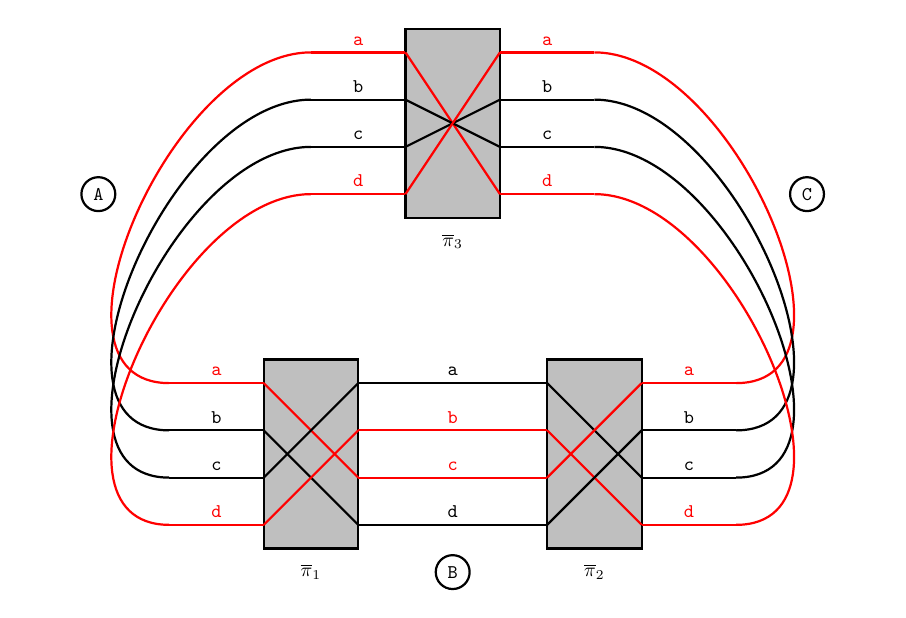
\begin{tikzpicture}[thick, scale=0.6, every node/.style={scale=0.7}]
			% Draw the box
			\draw[fill=lightgray] (2,-1.5) rectangle (4,2.5) node[midway] {};

			\node at (3, -2) {$\overline\pi_3$};

			% Draw the wires entering the box
			\draw[-, red] (0, 2) -- (2, 2) node[midway, above] {\texttt{a}};
			\draw[-] (0, 1) -- (2, 1) node[midway, above] {\texttt{b}};
			\draw[-] (0, 0) -- (2, 0) node[midway, above] {\texttt{c}};
			\draw[-, red] (0,-1) -- (2,-1) node[midway, above] {\texttt{d}};

			% Draw the wires exiting the box with crossed mappings
			\draw[-, red] (4, 2) -- (6,2) node[midway, above] {\texttt{a}};
			\draw[-] (4, 1) -- (6, 1) node[midway, above] {\texttt{b}};
			\draw[-] (4, 0) -- (6, 0) node[midway, above] {\texttt{c}};
			\draw[-, red] (4,-1) -- (6, -1) node[midway, above] {\texttt{d}};

			% Draw the lines inside the box to represent the mapping
			\draw[-, red] (2, 2) -- (4,-1);
			\draw[-] (2, 1) -- (4, 0);
			\draw[-] (2, 0) -- (4, 1);
			\draw[-, red] (2,-1) -- (4, 2);

			\draw[-, red] (0-3, 2-7) to[out=180, in=180] (0, 2) node[midway, above] {};
			\draw[-] (0-3, 1-7) to[out=180, in=180] (0, 1) node[midway, above] {};
			\draw[-] (0-3, 0-7) to[out=180, in=180] (0, 0) node[midway, above] {};
			\draw[-, red] (0-3, -1-7) to[out=180, in=180] (0, -1)
			node[midway, above] {};

			\draw[-, red] (6+3, 2-7) to[out=360, in=360] (6, 2) node[midway, above] {};
			\draw[-] (6+3, 1-7) to[out=360, in=360] (6, 1) node[midway, above] {};
			\draw[-] (6+3, 0-7) to[out=360, in=360] (6, 0) node[midway, above] {};
			\draw[-, red] (6+3, -1-7) to[out=360, in=360] (6, -1)
			node[midway, above] {};

			\draw[fill=lightgray] (2-3,-1.5-7) rectangle (4-3,2.5-7) node[midway] {};

			\node at (3-3, -2-7) {$\overline\pi_1$};

			% Draw the wires entering the box
			\draw[-, red] (0-3, 2-7) -- (2-3, 2-7) node[midway, above] {\texttt{a}};
			\draw[-] (0-3, 1-7) -- (2-3, 1-7) node[midway, above] {\texttt{b}};
			\draw[-] (0-3, 0-7) -- (2-3, 0-7) node[midway, above] {\texttt{c}};
			\draw[-, red] (0-3,-1-7) -- (2-3,-1-7) node[midway, above] {\texttt{d}};

			% Draw the wires exiting the box
			\draw[-] (4-3, 2-7) -- (6-3,2-7) node[right, above] {\texttt{a}};
			\draw[-, red] (4-3, 1-7) -- (6-3, 1-7) node[right, above] {\texttt{b}};
			\draw[-, red] (4-3, 0-7) -- (6-3, 0-7) node[right, above] {\texttt{c}};
			\draw[-] (4-3,-1-7) -- (6-3, -1-7) node[right, above] {\texttt{d}};

			% Draw the lines inside the box to represent the mapping
			\draw[-, red] (2-3, 2-7) -- (4-3, 0-7);
			\draw[-] (2-3, 1-7) -- (4-3, -1-7);
			\draw[-] (2-3, 0-7) -- (4-3, 2-7);
			\draw[-, red] (2-3,-1-7) -- (4-3, 1-7);

			\draw[fill=lightgray] (2+3,-1.5-7) rectangle (4+3,2.5-7) node[midway] {};

			\node at (3+3, -2-7) {$\overline\pi_2$};

			% Draw the wires entering the box
			\draw[-] (0+3, 2-7) -- (2+3, 2-7) node[midway, above] {};
			\draw[-, red] (0+3, 1-7) -- (2+3, 1-7) node[midway, above] {};
			\draw[-, red] (0+3, 0-7) -- (2+3, 0-7) node[midway, above] {};
			\draw[-] (0+3,-1-7) -- (2+3,-1-7) node[midway, above] {};

			% Draw the wires exiting the box
			\draw[-, red] (4+3, 2-7) -- (6+3,2-7) node[midway, above] {\texttt{a}};
			\draw[-] (4+3, 1-7) -- (6+3, 1-7) node[midway, above] {\texttt{b}};
			\draw[-] (4+3, 0-7) -- (6+3, 0-7) node[midway, above] {\texttt{c}};
			\draw[-, red] (4+3,-1-7) -- (6+3, -1-7) node[midway, above] {\texttt{d}};

			\draw[-] (2+3, 2-7) -- (4+3, 0-7);
			\draw[-, red] (2+3, 1-7) -- (4+3, -1-7);
			\draw[-, red] (2+3, 0-7) -- (4+3, 2-7);
			\draw[-] (2+3,-1-7) -- (4+3, 1-7);

			\node[draw,circle] at (-4.5, -1) {\texttt{A}};
			\node[draw,circle] at (3, -9) {\texttt{B}};
			\node[draw,circle] at (10.5, -1) {\texttt{C}};

		\end{tikzpicture}.
	\end{center}
\end{frame}


\begin{frame}
	\begin{center}
		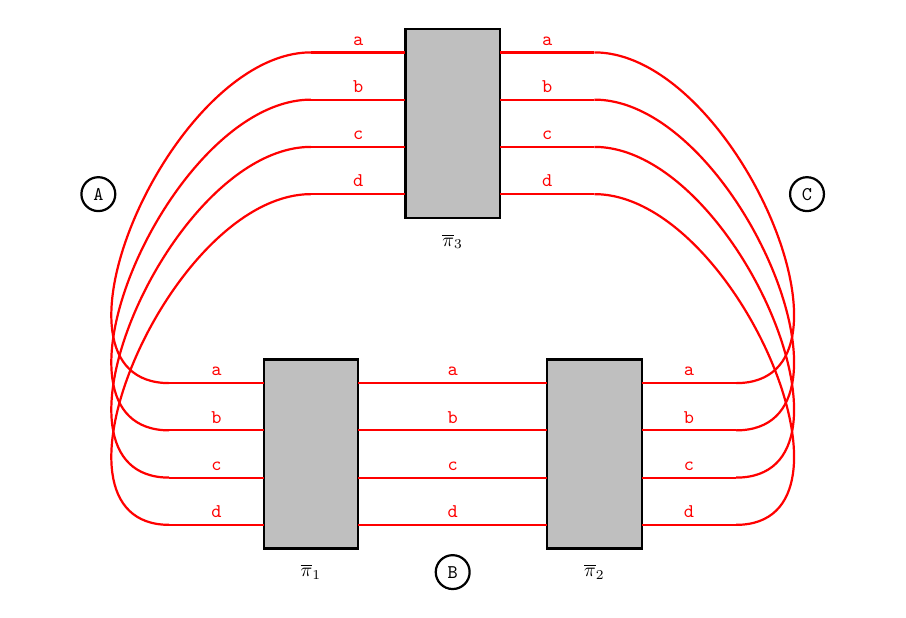
\begin{tikzpicture}[thick, scale=0.6, every node/.style={scale=0.7}]
			% Draw the box
			\draw[fill=lightgray] (2,-1.5) rectangle (4,2.5) node[midway] {};

			\node at (3, -2) {$\overline\pi_3$};

			% Draw the wires entering the box
			\draw[-, red] (0, 2) -- (2, 2) node[midway, above] {\texttt{a}};
			\draw[-, red] (0, 1) -- (2, 1) node[midway, above] {\texttt{b}};
			\draw[-, red] (0, 0) -- (2, 0) node[midway, above] {\texttt{c}};
			\draw[-, red] (0,-1) -- (2,-1) node[midway, above] {\texttt{d}};

			% Draw the wires exiting the box with crossed mappings
			\draw[-, red] (4, 2) -- (6,2) node[midway, above] {\texttt{a}};
			\draw[-, red] (4, 1) -- (6, 1) node[midway, above] {\texttt{b}};
			\draw[-, red] (4, 0) -- (6, 0) node[midway, above] {\texttt{c}};
			\draw[-, red] (4,-1) -- (6, -1) node[midway, above] {\texttt{d}};

			% % Draw the lines inside the box to represent the mapping
			% \draw[-, red] (2, 2) -- (4,-1);
			% \draw[-] (2, 1) -- (4, 0);
			% \draw[-] (2, 0) -- (4, 1);
			% \draw[-, red] (2,-1) -- (4, 2);

			\draw[-, red] (0-3, 2-7) to[out=180, in=180] (0, 2) node[midway, above] {};
			\draw[-, red] (0-3, 1-7) to[out=180, in=180] (0, 1) node[midway, above] {};
			\draw[-, red] (0-3, 0-7) to[out=180, in=180] (0, 0) node[midway, above] {};
			\draw[-, red] (0-3, -1-7) to[out=180, in=180] (0, -1)
			node[midway, above] {};

			\draw[-, red] (6+3, 2-7) to[out=360, in=360] (6, 2) node[midway, above] {};
			\draw[-, red] (6+3, 1-7) to[out=360, in=360] (6, 1) node[midway, above] {};
			\draw[-, red] (6+3, 0-7) to[out=360, in=360] (6, 0) node[midway, above] {};
			\draw[-, red] (6+3, -1-7) to[out=360, in=360] (6, -1)
			node[midway, above] {};

			\draw[fill=lightgray] (2-3,-1.5-7) rectangle (4-3,2.5-7) node[midway] {};

			\node at (3-3, -2-7) {$\overline\pi_1$};

			% Draw the wires entering the box
			\draw[-, red] (0-3, 2-7) -- (2-3, 2-7) node[midway, above] {\texttt{a}};
			\draw[-, red] (0-3, 1-7) -- (2-3, 1-7) node[midway, above] {\texttt{b}};
			\draw[-, red] (0-3, 0-7) -- (2-3, 0-7) node[midway, above] {\texttt{c}};
			\draw[-, red] (0-3,-1-7) -- (2-3,-1-7) node[midway, above] {\texttt{d}};

			% Draw the wires exiting the box
			\draw[-, red] (4-3, 2-7) -- (6-3,2-7) node[right, above] {\texttt{a}};
			\draw[-, red] (4-3, 1-7) -- (6-3, 1-7) node[right, above] {\texttt{b}};
			\draw[-, red] (4-3, 0-7) -- (6-3, 0-7) node[right, above] {\texttt{c}};
			\draw[-, red] (4-3,-1-7) -- (6-3, -1-7) node[right, above] {\texttt{d}};

			% % Draw the lines inside the box to represent the mapping
			% \draw[-, red] (2-3, 2-7) -- (4-3, 0-7);
			% \draw[-] (2-3, 1-7) -- (4-3, -1-7);
			% \draw[-] (2-3, 0-7) -- (4-3, 2-7);
			% \draw[-, red] (2-3,-1-7) -- (4-3, 1-7);

			\draw[fill=lightgray] (2+3,-1.5-7) rectangle (4+3,2.5-7) node[midway] {};

			\node at (3+3, -2-7) {$\overline\pi_2$};

			% Draw the wires entering the box
			\draw[-, red] (0+3, 2-7) -- (2+3, 2-7) node[midway, above] {};
			\draw[-, red] (0+3, 1-7) -- (2+3, 1-7) node[midway, above] {};
			\draw[-, red] (0+3, 0-7) -- (2+3, 0-7) node[midway, above] {};
			\draw[-, red] (0+3,-1-7) -- (2+3,-1-7) node[midway, above] {};

			% Draw the wires exiting the box
			\draw[-, red] (4+3, 2-7) -- (6+3,2-7) node[midway, above] {\texttt{a}};
			\draw[-, red] (4+3, 1-7) -- (6+3, 1-7) node[midway, above] {\texttt{b}};
			\draw[-, red] (4+3, 0-7) -- (6+3, 0-7) node[midway, above] {\texttt{c}};
			\draw[-, red] (4+3,-1-7) -- (6+3, -1-7) node[midway, above] {\texttt{d}};

			% \draw[-] (2+3, 2-7) -- (4+3, 0-7);
			% \draw[-, red] (2+3, 1-7) -- (4+3, -1-7);
			% \draw[-, red] (2+3, 0-7) -- (4+3, 2-7);
			% \draw[-] (2+3,-1-7) -- (4+3, 1-7);

			\node[draw,circle] at (-4.5, -1) {\texttt{A}};
			\node[draw,circle] at (3, -9) {\texttt{B}};
			\node[draw,circle] at (10.5, -1) {\texttt{C}};

		\end{tikzpicture}
	\end{center}
\end{frame}

\begin{frame}{Running the Bombe}
	\begin{center}
    \scalebox{0.8}{
		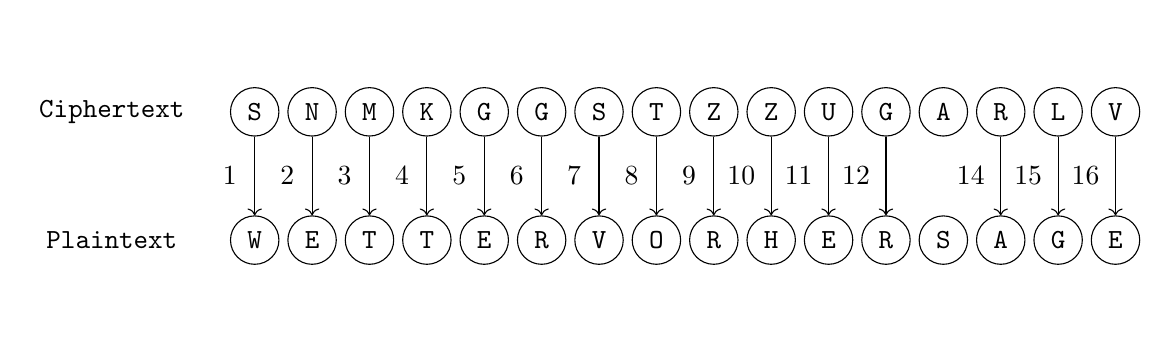
\begin{tikzpicture}[node distance=1cm, every node/.style={draw,
						circle, minimum height=0.1cm, minimum width=0.1cm}]

			% Centering the diagram
			\node (a1) [] {\texttt{S}};
			\node (a2) [right=0.1cm of a1] {\texttt{N}};
			\node (a3) [right=0.1cm of a2] {\texttt{M}};
                \node (a4) [right=0.1cm of a3] {\texttt{K}};    
                \node (a5) [right=0.1cm of a4] {\texttt{G}}; 
                \node (a6) [right=0.1cm of a5] {\texttt{G}}; 
                \node (a7) [right=0.1cm of a6] {\texttt{S}}; 
                \node (a8) [right=0.1cm of a7] {\texttt{T}}; 
                \node (a9) [right=0.1cm of a8] {\texttt{Z}}; 
                \node (a10) [right=0.1cm of a9] {\texttt{Z}}; 
                \node (a11) [right=0.1cm of a10] {\texttt{U}}; 
                \node (a12) [right=0.1cm of a11] {\texttt{G}}; 
                \node (a13) [right=0.1cm of a12] {\texttt{A}}; 
                \node (a14) [right=0.1cm of a13] {\texttt{R}}; 
                \node (a15) [right=0.1cm of a14] {\texttt{L}}; 
                \node (a16) [right=0.1cm of a15] {\texttt{V}}; 
                

			% Nodes for ciphertext
			\node (x1) [below=1cm of a1] {\texttt{W}};
			\node (x2) [below=1cm of a2] {\texttt{E}};
			\node (x3) [below=1cm of a3] {\texttt{T}};
                \node (x4) [below=1cm of a4] {\texttt{T}};
                \node (x5) [below=1cm of a5] {\texttt{E}};
                \node (x6) [below=1cm of a6] {\texttt{R}};
                \node (x7) [below=1cm of a7] {\texttt{V}};
                \node (x8) [below=1cm of a8] {\texttt{O}};
                \node (x9) [below=1cm of a9] {\texttt{R}};
                \node (x10) [below=1cm of a10] {\texttt{H}};
                \node (x11) [below=1cm of a11] {\texttt{E}};
                \node (x12) [below=1cm of a12] {\texttt{R}};
                \node (x13) [below=1cm of a13] {\texttt{S}};
                \node (x14) [below=1cm of a14] {\texttt{A}};
                \node (x15) [below=1cm of a15] {\texttt{G}};
                \node (x16) [below=1cm of a16] {\texttt{E}};
                

			% Arrows for mapping
			\draw[->] (a1) -- (x1) node[midway, left, draw=none, fill=none] {1};
			\draw[->] (a2) -- (x2) node[midway, left, draw=none, fill=none] {2};
			\draw[->] (a3) -- (x3) node[midway, left, draw=none, fill=none] {3};
                \draw[->] (a4) -- (x4) node[midway, left, draw=none, fill=none] {4};
                \draw[->] (a5) -- (x5) node[midway, left, draw=none, fill=none] {5};
                \draw[->] (a6) -- (x6) node[midway, left, draw=none, fill=none] {6};
                \draw[->] (a7) -- (x7) node[midway, left, draw=none, fill=none] {7};
                \draw[->] (a8) -- (x8) node[midway, left, draw=none, fill=none] {8};
                \draw[->] (a9) -- (x9) node[midway, left, draw=none, fill=none] {9};
                \draw[->] (a10) -- (x10) node[midway, left, draw=none, fill=none] {10};
                \draw[->] (a11) -- (x11) node[midway, left, draw=none, fill=none] {11};
                \draw[->] (a12) -- (x12) node[midway, left, draw=none, fill=none] {12};
                \draw[->] (a14) -- (x14) node[midway, left, draw=none, fill=none] {14};
                \draw[->] (a15) -- (x15) node[midway, left, draw=none, fill=none] {15};
                \draw[->] (a16) -- (x16) node[midway, left, draw=none, fill=none] {16};

                 \node[draw=none] at ([xshift=-1.5cm]a1.west) {\texttt{Ciphertext }};
                 \node[draw=none] at ([xshift=-1.5cm]x1.west) {\texttt{Plaintext  }};

		\end{tikzpicture}
        }
        \blfootnote{Thanks to Martin Gillow for the example.}
	\end{center}
\end{frame}

\begin{frame}{Running the Bombe}
	\begin{center}
		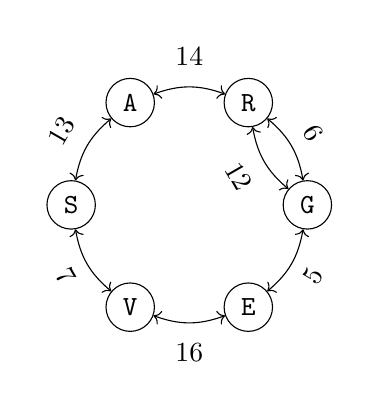
\begin{tikzpicture}[node distance=1cm, every node/.style={draw,
						circle, minimum height=0.1cm, minimum width=0.1cm}]
			\node (R) at (60:1.5) {$\texttt{R}$};
			\node (A) at (120:1.5) {$\texttt{A}$};
			\node (S) at (180:1.5) {$\texttt{S}$};
                \node (V) at (240:1.5) {$\texttt{V}$};
                \node (E) at (300:1.5) {$\texttt{E}$};
                \node (G) at (360:1.5) {$\texttt{G}$};
            

			\draw[<->, bend right=20] (R) to node[midway, sloped, draw=none, above] {14} (A);
			\draw[<->, bend right=20] (A) to node[midway, sloped,draw=none, above] {13} (S);
			\draw[<->, bend right=20] (S) to node[midway, sloped,draw=none, below] {7} (V);
                \draw[<->, bend right=20] (V) to node[midway, sloped,draw=none, below] {16} (E);
                \draw[<->, bend right=20] (E) to node[midway, sloped,draw=none, below] {5} (G);
                \draw[<->, bend right=20] (G) to node[midway, sloped,draw=none, above] {6} (R);
                \draw[<->, bend left=20] (G) to node[midway, sloped, draw=none,below] {12} (R);
		\end{tikzpicture}
	\end{center}
\end{frame}

\begin{frame}{Running the Bombe}
	\begin{center}
		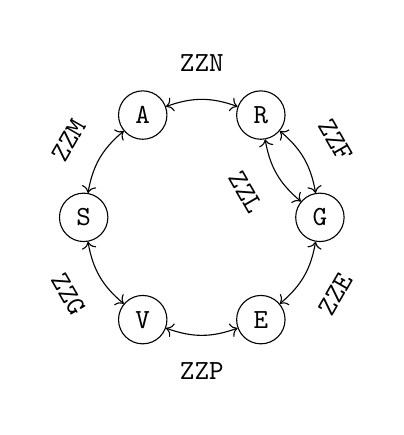
\begin{tikzpicture}[node distance=1cm, every node/.style={draw,
						circle, minimum height=0.1cm, minimum width=0.1cm}]
			\node (R) at (60:1.5) {$\texttt{R}$};
			\node (A) at (120:1.5) {$\texttt{A}$};
			\node (S) at (180:1.5) {$\texttt{S}$};
                \node (V) at (240:1.5) {$\texttt{V}$};
                \node (E) at (300:1.5) {$\texttt{E}$};
                \node (G) at (360:1.5) {$\texttt{G}$};
            

			\draw[<->, bend right=20] (R) to node[midway, sloped, draw=none, above] {\texttt{ZZN}} (A);
			\draw[<->, bend right=20] (A) to node[midway, sloped,draw=none, above] {\texttt{ZZM}} (S);
			\draw[<->, bend right=20] (S) to node[midway, sloped,draw=none, below] {\texttt{ZZG}} (V);
                \draw[<->, bend right=20] (V) to node[midway, sloped,draw=none, below] {\texttt{ZZP}} (E);
                \draw[<->, bend right=20] (E) to node[midway, sloped,draw=none, below] {\texttt{ZZE}} (G);
                \draw[<->, bend right=20] (G) to node[midway, sloped,draw=none, above] {\texttt{ZZF}} (R);
                \draw[<->, bend left=20] (G) to node[midway, sloped, draw=none,below] {\texttt{ZZL}} (R);
		\end{tikzpicture}
	\end{center}
\end{frame}

\begin{frame}{Running the Bombe}
\begin{center}
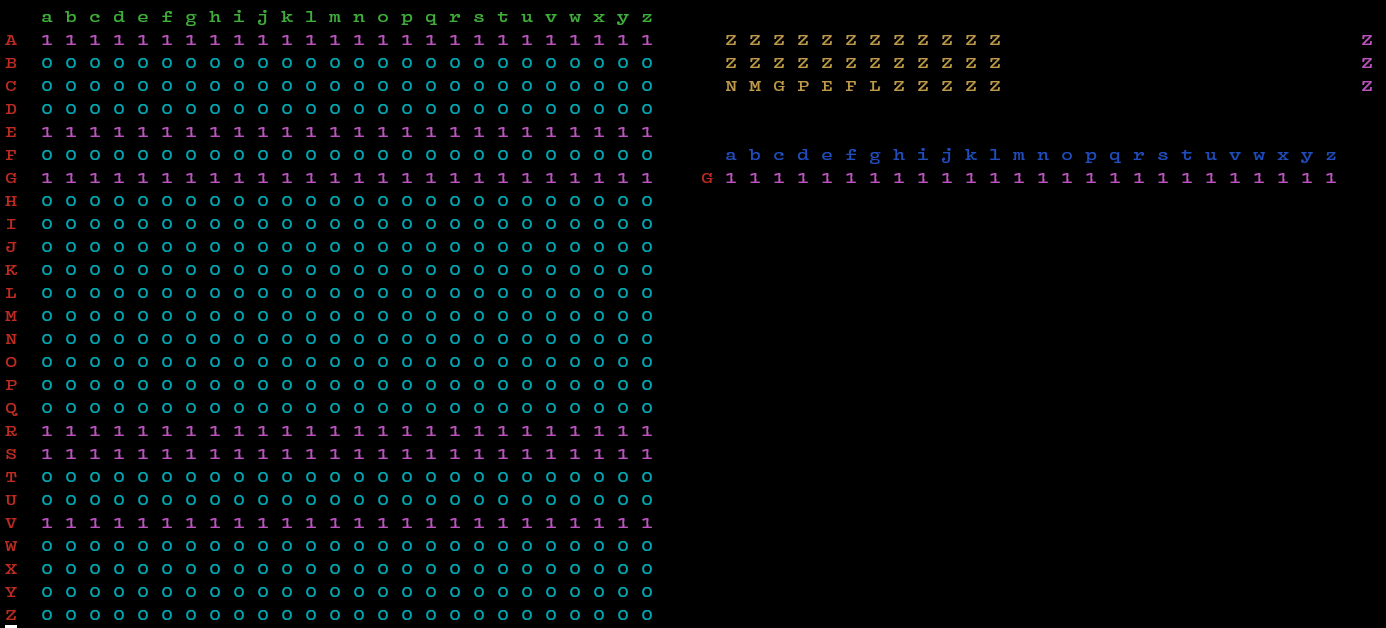
\includegraphics[scale=0.38]{paper/images/bombe_sim_1.png}
\end{center}
\end{frame}


\begin{frame}{Running the Bombe}
\begin{center}
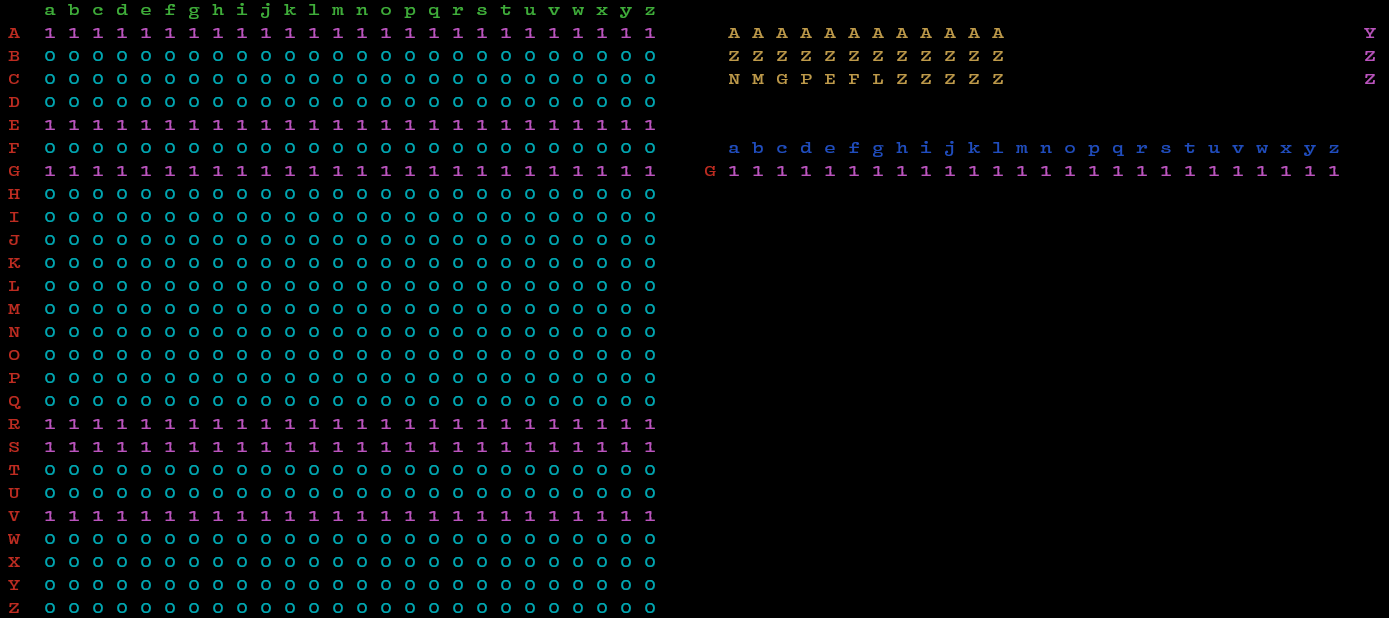
\includegraphics[scale=0.38]{paper/images/bombe_sim_2.png}
\end{center}
\end{frame}


\begin{frame}{Running the Bombe}
\begin{center}
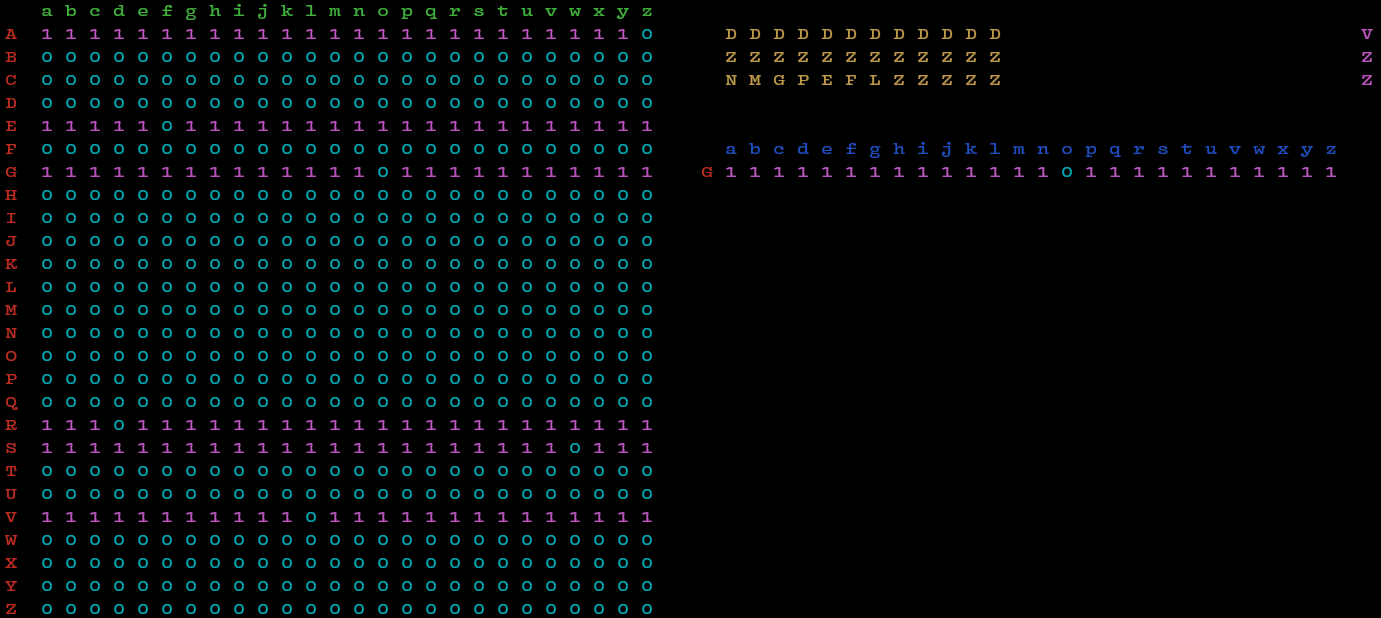
\includegraphics[scale=0.36]{paper/images/bombe_sim_3.png}
\end{center}
\blfootnote{Note that we have a {\bf{normal stop}} at hypothesis $S(\texttt{G}) = \texttt{O}$.}
\end{frame}


\begin{frame}{Running the Bombe}
\begin{center}
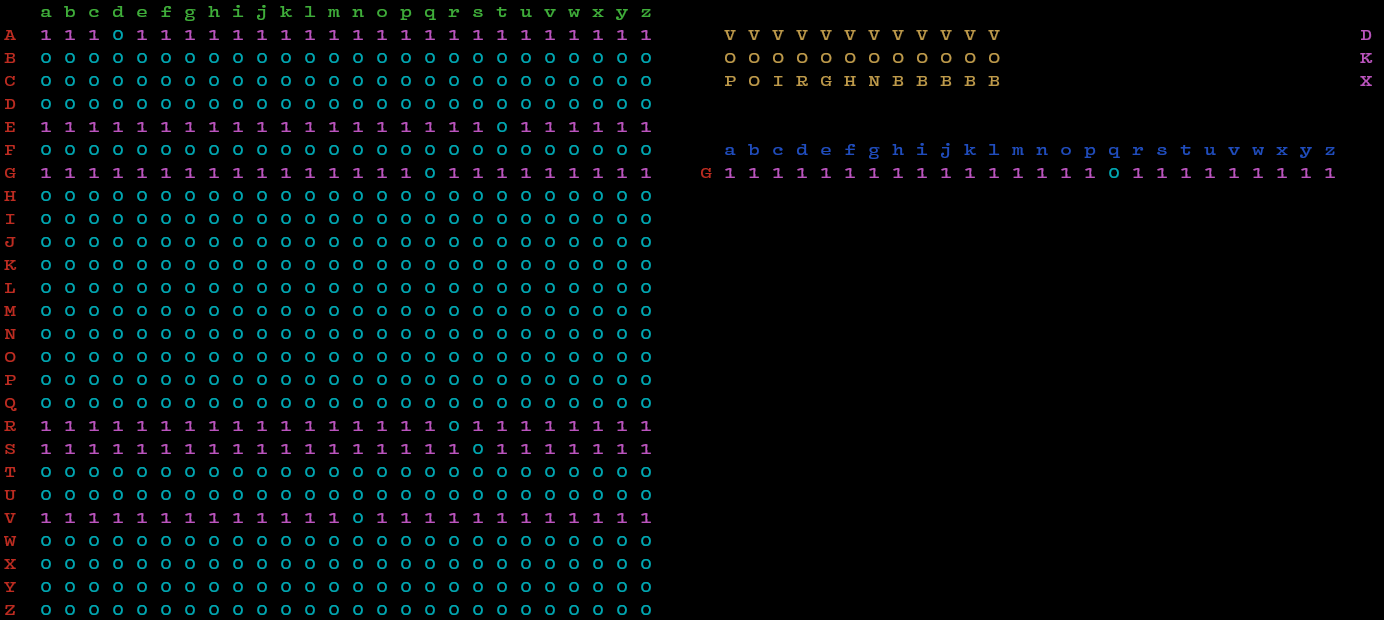
\includegraphics[scale=0.38]{paper/images/bombe_sim_4.png}
\end{center}
\end{frame}

\part{}
\section{Stops}

\begin{frame}[fragile]{}
	\Huge
	\begin{center}
		Analyzing the Bombe's Efficacy
	\end{center}
\end{frame}

\begin{frame}[fragile]{Normal Stops}
	For his analysis, Turing defines a \textbf{normal stop} as, ``positions at which by altering the point at which the current
	enters the diagonal board, one can make 25 relays close.''
\end{frame}

\begin{frame}[fragile]{Turing's Model}
	Turing computes the \emph{expected number of normal stops over all steckering hypothesis} as,
	\begin{center}
		$26^{4-c}$,
	\end{center}
	where $c$ is the number of loops (or closures) in a menu.
\end{frame}

\begin{frame}[fragile]{Issues}
	\begin{enumerate}
		\item Does not consider abnormal stops (under-counts).
		      \vspace{1em}
		\item Repeatedly considers stops with multiple steckering hypotheses producing normal stops (over-counts).
	\end{enumerate}
\end{frame}


\begin{frame}[fragile]{Issues}
	For example, for two closures, Turing estimates $676$ stops.
	\\\\Via simulation we find, $715.79\pm2.25$ stops.
\end{frame}

\begin{frame}[fragile]{Cycle Type Model}
	To address these issues, we propose a new model based on a mixture of combinatoric analysis and simulation.
\end{frame}

\begin{frame}[fragile]{Parity}
	For one loop, we may try to find the expected number of stops by looking at the probability that a uniformly random permutation in $S_{26}$ forms a $26$ cycle.
	\\\\That is, \begin{center}
		$\frac{1}{26}$.
	\end{center}
\end{frame}

\begin{frame}[fragile]{Parity}
	\large
	But permutations generated by the Bombe are not uniformly random!
\end{frame}

\begin{frame}[fragile]{Parity}
	Each permutation $\overline\pi_i$ has a
	$2^{13}$ cycle type and thus odd parity.
	\\\\Then for a loop of length $4$,
	\begin{center}
		$\overline\pi = \overline\pi_4\overline\pi_3\overline\pi_2\overline\pi_1$
	\end{center}
	has even parity.
\end{frame}

\begin{frame}[fragile]{Parity}
	\large
	A $26$ cycle always has odd parity.
	\\\\Then a Bombe with $4$ Enigma machines in a loop must always produce a stop!
\end{frame}

\begin{frame}[fragile]{Parity}
	\large
	Thus we must consider not just the number of closures, but the number of Enigmas within each closure ($\ell$).
\end{frame}

\begin{frame}[fragile]{One Loop}
	For one loop, the problem is easy to address via a Monte Carlo simulation, and the results have low variance.
	\\\\We simply combine $\ell$ Enigma machines in a loop and examine if the cycle type is  not $26^1$, dividing by the total number of samples, to get the probability of a stop.
\end{frame}

\begin{frame}[fragile]{One Loop}
	\large
	While simulating, we will collect the distribution of cycle types formed by an arrangement of $\ell$ Enigma machines for later use.
\end{frame}

\begin{frame}[fragile]{One Loop}
	\begin{table}[H]
		\centering

		\begin{tabular}{|c|c|c|}
			\hline
			{\bf{ $\ell$ }} & {\bf{ Expected Stops }} & {\bf{ Simulated Stops }} \\
			\hline
			2               & 17576.00                & $17576.00 \pm 0.00$      \\
			\hline
			3               & 16246.63                & $16243.78 \pm 6.91$      \\
			\hline
			4               & 17576.00                & $17576.00 \pm 0.00$      \\
			\hline
			5               & 16224.88                & $16220.57 \pm 6.66$      \\
			\hline
			6               & 17576.00                & $17576.00 \pm 0.00$      \\
			\hline
			7               & 16222.69                & $16224.37 \pm 6.63$      \\
			\hline
			8               & 17576.00                & $17576.00 \pm 0.00$      \\
			\hline
			9               & 16223.75                & $16227.80 \pm 6.92$      \\
			\hline
			10              & 17576.00                & $17576.00 \pm 0.00$      \\
			\hline
			11              & 16224.53                & $16228.59 \pm 6.95$      \\
			\hline
			12              & 17576.00                & $17576.00 \pm 0.00$      \\
			\hline
		\end{tabular}
		\caption{Single-Loop Bombe Stop Probabilities for Loop Lengths
			$\ell=2$ to $\ell=12$}
	\end{table}
\end{frame}

\begin{frame}[fragile]{Two Loops}
	For two loops, the complexity of arrangements results in high variance and inaccurate results.
	\\\\We must somehow combine our one loop results in such a way as to produce two loop results.
\end{frame}

\begin{frame}{Two Loops}
	\begin{center}
		\scalebox{0.8}{
			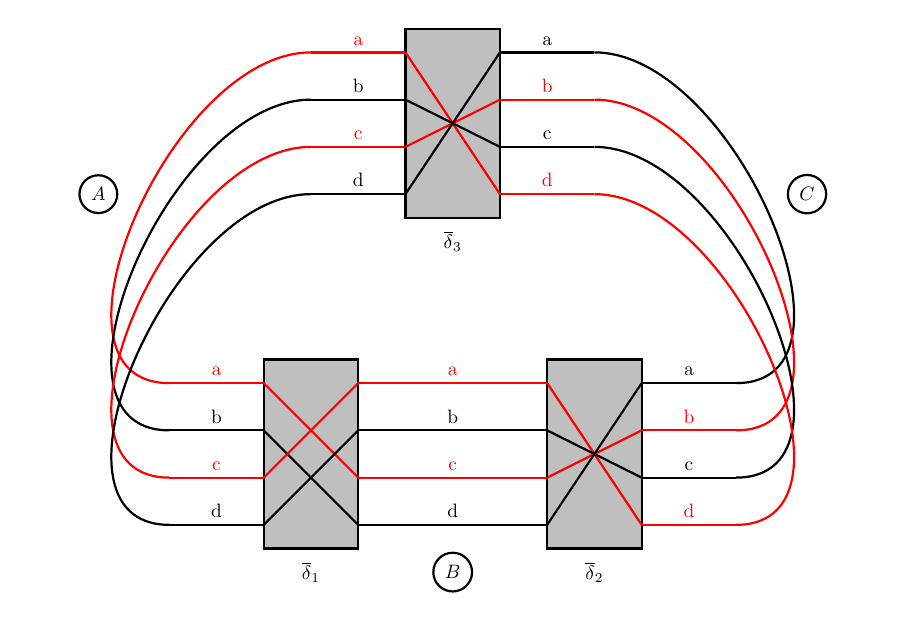
\begin{tikzpicture}[thick, scale=0.6, every node/.style={scale=0.7}]
				% Draw the box
				\draw[fill=lightgray] (2,-1.5) rectangle (4,2.5) node[midway] {};

				\node at (3, -2) {$\overline\delta_3$};

				% Draw the wires entering the box
				\draw[-, red] (0, 2) -- (2, 2) node[midway, above] {a};
				\draw[-] (0, 1) -- (2, 1) node[midway, above] {b};
				\draw[-, red] (0, 0) -- (2, 0) node[midway, above] {c};
				\draw[-] (0,-1) -- (2,-1) node[midway, above] {d};

				% Draw the wires exiting the box with crossed mappings
				\draw[-] (4, 2) -- (6,2) node[midway, above] {a};
				\draw[-, red] (4, 1) -- (6, 1) node[midway, above] {b};
				\draw[-] (4, 0) -- (6, 0) node[midway, above] {c};
				\draw[-, red] (4,-1) -- (6, -1) node[midway, above] {d};

				% Draw the lines inside the box to represent the mapping
				\draw[-, red] (2, 2) -- (4,-1);
				\draw[-] (2, 1) -- (4, 0);
				\draw[-, red] (2, 0) -- (4, 1);
				\draw[-] (2,-1) -- (4, 2);

				\draw[-, red] (0-3, 2-7) to[out=180, in=180] (0, 2) node[midway, above] {};
				\draw[-] (0-3, 1-7) to[out=180, in=180] (0, 1) node[midway, above] {};
				\draw[-, red] (0-3, 0-7) to[out=180, in=180] (0, 0) node[midway, above] {};
				\draw[-] (0-3, -1-7) to[out=180, in=180] (0, -1) node[midway, above] {};

				\draw[-] (6+3, 2-7) to[out=360, in=360] (6, 2) node[midway, above] {};
				\draw[-, red] (6+3, 1-7) to[out=360, in=360] (6, 1) node[midway, above] {};
				\draw[-] (6+3, 0-7) to[out=360, in=360] (6, 0) node[midway, above] {};
				\draw[-, red] (6+3, -1-7) to[out=360, in=360] (6, -1) node[midway, above] {};

				\draw[fill=lightgray] (2-3,-1.5-7) rectangle (4-3,2.5-7) node[midway] {};

				\node at (3-3, -2-7) {$\overline\delta_1$};

				% Draw the wires entering the box
				\draw[-, red] (0-3, 2-7) -- (2-3, 2-7) node[midway, above] {a};
				\draw[-] (0-3, 1-7) -- (2-3, 1-7) node[midway, above] {b};
				\draw[-, red] (0-3, 0-7) -- (2-3, 0-7) node[midway, above] {c};
				\draw[-] (0-3,-1-7) -- (2-3,-1-7) node[midway, above] {d};

				% Draw the wires exiting the box
				\draw[-, red] (4-3, 2-7) -- (6-3,2-7) node[right, above] {a};
				\draw[-] (4-3, 1-7) -- (6-3, 1-7) node[right, above] {b};
				\draw[-, red] (4-3, 0-7) -- (6-3, 0-7) node[right, above] {c};
				\draw[-] (4-3,-1-7) -- (6-3, -1-7) node[right, above] {d};

				% Draw the lines inside the box to represent the mapping
				\draw[-, red] (2-3, 2-7) -- (4-3, 0-7);
				\draw[-] (2-3, 1-7) -- (4-3, -1-7);
				\draw[-, red] (2-3, 0-7) -- (4-3, 2-7);
				\draw[-] (2-3,-1-7) -- (4-3, 1-7);

				\draw[fill=lightgray] (2+3,-1.5-7) rectangle (4+3,2.5-7) node[midway] {};

				\node at (3+3, -2-7) {$\overline\delta_2$};


				% Draw the wires entering the box
				\draw[-, red] (0+3, 2-7) -- (2+3, 2-7) node[midway, above] {};
				\draw[-] (0+3, 1-7) -- (2+3, 1-7) node[midway, above] {};
				\draw[-, red] (0+3, 0-7) -- (2+3, 0-7) node[midway, above] {};
				\draw[-] (0+3,-1-7) -- (2+3,-1-7) node[midway, above] {};

				% Draw the wires exiting the box
				\draw[-] (4+3, 2-7) -- (6+3,2-7) node[midway, above] {a};
				\draw[-, red] (4+3, 1-7) -- (6+3, 1-7) node[midway, above] {b};
				\draw[-] (4+3, 0-7) -- (6+3, 0-7) node[midway, above] {c};
				\draw[-, red] (4+3,-1-7) -- (6+3, -1-7) node[midway, above] {d};

				\draw[-, red] (2+3, 2-7) -- (4+3, -1-7);
				\draw[-] (2+3, 1-7) -- (4+3, 0-7);
				\draw[-, red] (2+3, 0-7) -- (4+3, 1-7);
				\draw[-] (2+3,-1-7) -- (4+3, 2-7);

				\node[draw,circle] at (-4.5, -1) {$A$};
				\node[draw,circle] at (3, -9) {$B$};
				\node[draw,circle] at (10.5, -1) {$C$};
			\end{tikzpicture}
		}
	\end{center}
	\begin{center}
		(\texttt{AC})(\texttt{BD})
	\end{center}
\end{frame}

\begin{frame}{Two Loops}
	\begin{center}
		\scalebox{0.8}{
			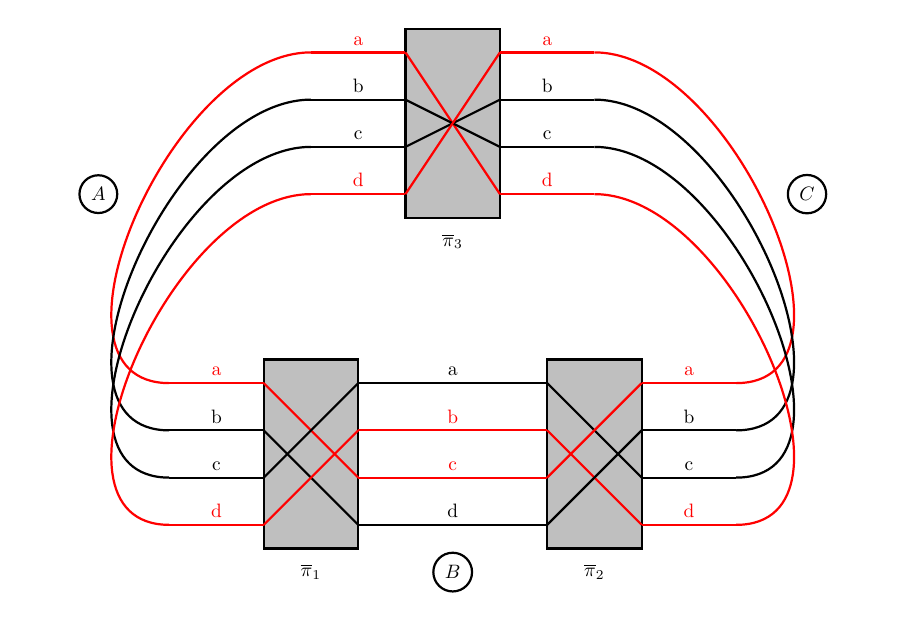
\begin{tikzpicture}[thick, scale=0.6, every node/.style={scale=0.7}]
				% Draw the box
				\draw[fill=lightgray] (2,-1.5) rectangle (4,2.5) node[midway] {};

				\node at (3, -2) {$\overline\pi_3$};

				% Draw the wires entering the box
				\draw[-, red] (0, 2) -- (2, 2) node[midway, above] {a};
				\draw[-] (0, 1) -- (2, 1) node[midway, above] {b};
				\draw[-] (0, 0) -- (2, 0) node[midway, above] {c};
				\draw[-, red] (0,-1) -- (2,-1) node[midway, above] {d};

				% Draw the wires exiting the box with crossed mappings
				\draw[-, red] (4, 2) -- (6,2) node[midway, above] {a};
				\draw[-] (4, 1) -- (6, 1) node[midway, above] {b};
				\draw[-] (4, 0) -- (6, 0) node[midway, above] {c};
				\draw[-, red] (4,-1) -- (6, -1) node[midway, above] {d};

				% Draw the lines inside the box to represent the mapping
				\draw[-, red] (2, 2) -- (4,-1);
				\draw[-] (2, 1) -- (4, 0);
				\draw[-] (2, 0) -- (4, 1);
				\draw[-, red] (2,-1) -- (4, 2);

				\draw[-, red] (0-3, 2-7) to[out=180, in=180] (0, 2) node[midway, above] {};
				\draw[-] (0-3, 1-7) to[out=180, in=180] (0, 1) node[midway, above] {};
				\draw[-] (0-3, 0-7) to[out=180, in=180] (0, 0) node[midway, above] {};
				\draw[-, red] (0-3, -1-7) to[out=180, in=180] (0, -1) node[midway, above] {};

				\draw[-, red] (6+3, 2-7) to[out=360, in=360] (6, 2) node[midway, above] {};
				\draw[-] (6+3, 1-7) to[out=360, in=360] (6, 1) node[midway, above] {};
				\draw[-] (6+3, 0-7) to[out=360, in=360] (6, 0) node[midway, above] {};
				\draw[-, red] (6+3, -1-7) to[out=360, in=360] (6, -1) node[midway, above] {};

				\draw[fill=lightgray] (2-3,-1.5-7) rectangle (4-3,2.5-7) node[midway] {};

				\node at (3-3, -2-7) {$\overline\pi_1$};

				% Draw the wires entering the box
				\draw[-, red] (0-3, 2-7) -- (2-3, 2-7) node[midway, above] {a};
				\draw[-] (0-3, 1-7) -- (2-3, 1-7) node[midway, above] {b};
				\draw[-] (0-3, 0-7) -- (2-3, 0-7) node[midway, above] {c};
				\draw[-, red] (0-3,-1-7) -- (2-3,-1-7) node[midway, above] {d};

				% Draw the wires exiting the box
				\draw[-] (4-3, 2-7) -- (6-3,2-7) node[right, above] {a};
				\draw[-, red] (4-3, 1-7) -- (6-3, 1-7) node[right, above] {b};
				\draw[-, red] (4-3, 0-7) -- (6-3, 0-7) node[right, above] {c};
				\draw[-] (4-3,-1-7) -- (6-3, -1-7) node[right, above] {d};

				% Draw the lines inside the box to represent the mapping
				\draw[-, red] (2-3, 2-7) -- (4-3, 0-7);
				\draw[-] (2-3, 1-7) -- (4-3, -1-7);
				\draw[-] (2-3, 0-7) -- (4-3, 2-7);
				\draw[-, red] (2-3,-1-7) -- (4-3, 1-7);

				\draw[fill=lightgray] (2+3,-1.5-7) rectangle (4+3,2.5-7) node[midway] {};

				\node at (3+3, -2-7) {$\overline\pi_2$};


				% Draw the wires entering the box
				\draw[-] (0+3, 2-7) -- (2+3, 2-7) node[midway, above] {};
				\draw[-, red] (0+3, 1-7) -- (2+3, 1-7) node[midway, above] {};
				\draw[-, red] (0+3, 0-7) -- (2+3, 0-7) node[midway, above] {};
				\draw[-] (0+3,-1-7) -- (2+3,-1-7) node[midway, above] {};

				% Draw the wires exiting the box
				\draw[-, red] (4+3, 2-7) -- (6+3,2-7) node[midway, above] {a};
				\draw[-] (4+3, 1-7) -- (6+3, 1-7) node[midway, above] {b};
				\draw[-] (4+3, 0-7) -- (6+3, 0-7) node[midway, above] {c};
				\draw[-, red] (4+3,-1-7) -- (6+3, -1-7) node[midway, above] {d};

				\draw[-] (2+3, 2-7) -- (4+3, 0-7);
				\draw[-, red] (2+3, 1-7) -- (4+3, -1-7);
				\draw[-, red] (2+3, 0-7) -- (4+3, 2-7);
				\draw[-] (2+3,-1-7) -- (4+3, 1-7);

				\node[draw,circle] at (-4.5, -1) {$A$};
				\node[draw,circle] at (3, -9) {$B$};
				\node[draw,circle] at (10.5, -1) {$C$};
			\end{tikzpicture}
		}
	\end{center}
	\begin{center}
		(\texttt{AD})(\texttt{BC})
	\end{center}
\end{frame}

\begin{frame}{Two Loops}
	\begin{center}
		\scalebox{0.8}{
			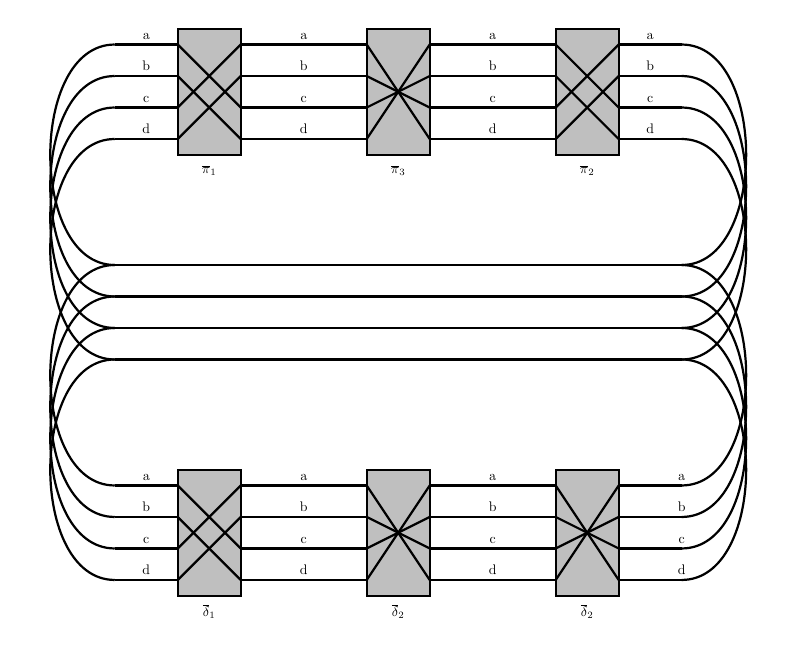
\begin{tikzpicture}[thick, scale=0.4, every node/.style={scale=0.5}]
				% Draw the box
				\draw[fill=lightgray] (2-6,-1.5) rectangle (4-6,2.5) node[midway] {};

				\node at (3-6, -2) {$\overline\pi_1$};

				% Draw the wires entering the box
				\draw[-] (0-6, 2) -- (2-6, 2) node[midway, above] {a};
				\draw[-] (0-6, 1) -- (2-6, 1) node[midway, above] {b};
				\draw[-] (0-6, 0) -- (2-6, 0) node[midway, above] {c};
				\draw[-] (0-6,-1) -- (2-6,-1) node[midway, above] {d};

				% Draw the wires exiting the box with crossed mappings
				\draw[-] (4-6, 2) -- (6-6,2) node[right, above] {a};
				\draw[-] (4-6, 1) -- (6-6, 1) node[right, above] {b};
				\draw[-] (4-6, 0) -- (6-6, 0) node[right, above] {c};
				\draw[-] (4-6,-1) -- (6-6, -1) node[right, above] {d};

				% Draw the lines inside the box to represent the mapping
				\draw[-] (2-6, 2) -- (4-6,0);
				\draw[-] (2-6, 1) -- (4-6, -1);
				\draw[-] (2-6, 0) -- (4-6, 2);
				\draw[-] (2-6,-1) -- (4-6, 1);

				\draw[fill=lightgray] (2,-1.5) rectangle (4,2.5) node[midway] {};

				\node at (3, -2) {$\overline\pi_3$};

				% Draw the wires entering the box
				\draw[-] (0, 2) -- (2, 2) node[midway, above] {};
				\draw[-] (0, 1) -- (2, 1) node[midway, above] {};
				\draw[-] (0, 0) -- (2, 0) node[midway, above] {};
				\draw[-] (0,-1) -- (2,-1) node[midway, above] {};

				% Draw the wires exiting the box
				\draw[-] (4, 2) -- (6,2) node[right, above] {a};
				\draw[-] (4, 1) -- (6, 1) node[right, above] {b};
				\draw[-] (4, 0) -- (6, 0) node[right, above] {c};
				\draw[-] (4,-1) -- (6, -1) node[right, above] {d};

				% Draw the lines inside the box to represent the mapping
				\draw[-] (2, 2) -- (4, -1);
				\draw[-] (2, 1) -- (4, 0);
				\draw[-] (2, 0) -- (4, 1);
				\draw[-] (2,-1) -- (4, 2);

				\draw[fill=lightgray] (2+6,-1.5) rectangle (4+6,2.5) node[midway] {};

				\node at (3+6, -2) {$\overline\pi_2$};


				% Draw the wires entering the box
				\draw[-] (0+6, 2) -- (2+6, 2) node[midway, above] {};
				\draw[-] (0+6, 1) -- (2+6, 1) node[midway, above] {};
				\draw[-] (0+6, 0) -- (2+6, 0) node[midway, above] {};
				\draw[-] (0+6,-1) -- (2+6,-1) node[midway, above] {};

				% Draw the wires exiting the box
				\draw[-] (4+6, 2) -- (6+6,2) node[midway, above] {a};
				\draw[-] (4+6, 1) -- (6+6, 1) node[midway, above] {b};
				\draw[-] (4+6, 0) -- (6+6, 0) node[midway, above] {c};
				\draw[-] (4+6,-1) -- (6+6, -1) node[midway, above] {d};

				\draw[-] (2+6, 2) -- (4+6, 0);
				\draw[-] (2+6, 1) -- (4+6, -1);
				\draw[-] (2+6, 0) -- (4+6, 2);
				\draw[-] (2+6,-1) -- (4+6, 1);

				\draw[-] (0-6, 2) to[out=180, in=180] (-6, 2-7) node[midway, above] {};
				\draw[-] (0-6, 1) to[out=180, in=180] (-6, 1-7) node[midway, above] {};
				\draw[-] (0-6, 0) to[out=180, in=180] (-6, 0-7) node[midway, above] {};
				\draw[-] (0-6, -1) to[out=180, in=180] (-6, -1-7) node[midway, above] {};

				\draw[-] (6+6, 2) to[out=360, in=360] (6+6, 2-7) node[midway, above] {};
				\draw[-] (6+6, 1) to[out=360, in=360] (6+6, 1-7) node[midway, above] {};
				\draw[-] (6+6, 0) to[out=360, in=360] (6+6, 0-7) node[midway, above] {};
				\draw[-] (6+6, -1) to[out=360, in=360] (6+6, -1-7) node[midway, above] {};

				\draw[-] (-6, 2-7) to (6+6, 2-7) node[midway, above] {};
				\draw[-] (-6, 1-7) to (6+6, 1-7) node[midway, above] {};
				\draw[-] (-6, 0-7) to (6+6, 0-7) node[midway, above] {};
				\draw[-] (-6, -1-7) to (6+6, -1-7) node[midway, above] {};

				\draw[-] (0-6, 2-14) to[out=180, in=180] (-6, 2-7) node[midway, above] {};
				\draw[-] (0-6, 1-14) to[out=180, in=180] (-6, 1-7) node[midway, above] {};
				\draw[-] (0-6, 0-14) to[out=180, in=180] (-6, 0-7) node[midway, above] {};
				\draw[-] (0-6, -1-14) to[out=180, in=180] (-6, -1-7) node[midway, above] {};

				\draw[-] (6+6, 2-14) to[out=360, in=360] (6+6, 2-7) node[midway, above] {};
				\draw[-] (6+6, 1-14) to[out=360, in=360] (6+6, 1-7) node[midway, above] {};
				\draw[-] (6+6, 0-14) to[out=360, in=360] (6+6, 0-7) node[midway, above] {};
				\draw[-] (6+6, -1-14) to[out=360, in=360] (6+6, -1-7) node[midway, above] {};

				\draw[fill=lightgray] (2-6,-1.5-14) rectangle (4-6,2.5-14) node[midway] {};

				% \node at (3-6, -2) {$\overline\sigma_3$};

				% Draw the wires entering the box
				\draw[-] (0-6, 2-14) -- (2-6, 2-14) node[midway, above] {a};
				\draw[-] (0-6, 1-14) -- (2-6, 1-14) node[midway, above] {b};
				\draw[-] (0-6, 0-14) -- (2-6, 0-14) node[midway, above] {c};
				\draw[-] (0-6,-1-14) -- (2-6,-1-14) node[midway, above] {d};

				% Draw the wires exiting the box with crossed mappings
				\draw[-] (4-6, 2-14) -- (6-6,2-14) node[right, above] {a};
				\draw[-] (4-6, 1-14) -- (6-6, 1-14) node[right, above] {b};
				\draw[-] (4-6, 0-14) -- (6-6, 0-14) node[right, above] {c};
				\draw[-] (4-6,-1-14) -- (6-6, -1-14) node[right, above] {d};

				% Draw the lines inside the box to represent the mapping
				\draw[-] (2-6, 2-14) -- (4-6,0-14);
				\draw[-] (2-6, 1-14) -- (4-6, -1-14);
				\draw[-] (2-6, 0-14) -- (4-6, 2-14);
				\draw[-] (2-6,-1-14) -- (4-6, 1-14);

				\node at (3-6, -2-14) {$\overline\delta_1$};

				\draw[fill=lightgray] (2,-1.5-14) rectangle (4,2.5-14) node[midway] {};

				\node at (3, -2-14) {$\overline\delta_2$};

				% Draw the wires entering the box
				\draw[-] (0, 2-14) -- (2, 2-14) node[midway, above] {};
				\draw[-] (0, 1-14) -- (2, 1-14) node[midway, above] {};
				\draw[-] (0, 0-14) -- (2, 0-14) node[midway, above] {};
				\draw[-] (0,-1-14) -- (2,-1-14) node[midway, above] {};

				% Draw the wires exiting the box
				\draw[-] (4, 2-14) -- (6,2-14) node[right, above] {a};
				\draw[-] (4, 1-14) -- (6, 1-14) node[right, above] {b};
				\draw[-] (4, 0-14) -- (6, 0-14) node[right, above] {c};
				\draw[-] (4,-1-14) -- (6, -1-14) node[right, above] {d};

				% Draw the lines inside the box to represent the mapping
				\draw[-] (2, 2-14) -- (4, -1-14);
				\draw[-] (2, 1-14) -- (4, 0-14);
				\draw[-] (2, 0-14) -- (4, 1-14);
				\draw[-] (2,-1-14) -- (4, 2-14);

				\draw[fill=lightgray] (2+6,-1.5-14) rectangle (4+6,2.5-14) node[midway] {};

				% \node at (3, -2-14) {$\delta_3$};

				% Draw the wires entering the box
				\draw[-] (0+6, 2-14) -- (2+6, 2-14) node[midway, above] {};
				\draw[-] (0+6, 1-14) -- (2+6, 1-14) node[midway, above] {};
				\draw[-] (0+6, 0-14) -- (2+6, 0-14) node[midway, above] {};
				\draw[-] (0+6,-1-14) -- (2+6,-1-14) node[midway, above] {};

				% Draw the wires exiting the box
				\draw[-] (4+6, 2-14) -- (6+6,2-14) node[right, above] {a};
				\draw[-] (4+6, 1-14) -- (6+6, 1-14) node[right, above] {b};
				\draw[-] (4+6, 0-14) -- (6+6, 0-14) node[right, above] {c};
				\draw[-] (4+6,-1-14) -- (6+6, -1-14) node[right, above] {d};

				% Draw the lines inside the box to represent the mapping
				\draw[-] (2+6, 2-14) -- (4+6, -1-14);
				\draw[-] (2+6, 1-14) -- (4+6, 0-14);
				\draw[-] (2+6, 0-14) -- (4+6, 1-14);
				\draw[-] (2+6,-1-14) -- (4+6, 2-14);

				\node at (3+6, -2-14) {$\overline\delta_2$};
				% \node[draw,circle] at (-4.5, -1) {$A$};
				% \node[draw,circle] at (3, -9) {$B$};
				% \node[draw,circle] at (10.5, -1) {$C$};
			\end{tikzpicture}
		}

	\end{center}
\end{frame}

\begin{frame}{Two Loops}
	\begin{itemize}
		\item Does ``cycle type'' have meaning here?
		      \pause
		      \vspace{1em}
		\item Is this arrangement connected?
	\end{itemize}
\end{frame}

\begin{frame}{Orbits}
	For $\sigma_1,\dots,\sigma_k\in S_n$, the subgroup $\langle \sigma_1,\dots,\sigma_k \rangle$ has a natural group action on $\mathbb{N}_n$ by,
	\begin{align*}
		\phi: \langle \sigma_1,\dots,\sigma_k \rangle \times \mathbb{N}_n & \to \mathbb{N}_n \\
		(\rho, i)                                                         & \mapsto \rho(i)
	\end{align*}
\end{frame}

\begin{frame}{Orbits}

	Then for a single $\sigma\in S_n$, the orbits of $\langle\sigma\rangle$ are just
	\begin{center}
		$\langle\sigma\rangle/\phi = \{\{\sigma^k(i)\text{ }|\text{ }\forall\text{ }k\in\mathbb{Z}\}\text{ }|\text{ }\forall\text{ }i\in\mathbb{N}_n\}$
	\end{center}

\end{frame}

\begin{frame}{Orbits}
	That is, if $\sigma$ has cycles $(\texttt{AB})(\texttt{CD})$, then $\langle\sigma\rangle$ will have orbits $\{\{\texttt{A},\texttt{B}\},\{\texttt{C},\texttt{D}\}\}$
\end{frame}

\begin{frame}{Orbits}
    For more loops $\overline\pi$ and $\overline\delta$, we can view the orbits of $\langle\overline\pi, \overline\delta\rangle$ to see which wires electrify each other.
\end{frame}


\begin{frame}{Two Loops}
	\begin{itemize}
		\item Does ``cycle type'' have meaning here?
		      \pause
		      \begin{itemize}
			      \item Think in terms of orbits of $\langle\overline\pi, \overline\delta\rangle$ instead.
		      \end{itemize}
		      \pause
		      \vspace{1em}
		\item Is this arrangement connected?
	\end{itemize}
\end{frame}

\begin{frame}{Transitivity}
	If we have two loops $\overline\pi$ and $\overline\delta$, the orbits of $\langle\overline\pi, \overline\delta\rangle$ will tell us which wires are reachable from one another.
	\pause
	\\\\If there is only a single orbit $\{\texttt{A}, \texttt{B},\dots, \texttt{Z}\}$, then our arrangement is connected.
	\pause
	\\\\When this happens we say $\langle\overline\pi, \overline\delta \rangle$ is a \textbf{transitive} subgroup of $S_n$.
\end{frame}

\begin{frame}{Two Loops}
	\begin{itemize}
		\item Does ``cycle type'' have meaning here?
		      \begin{itemize}
			      \item Think in terms of orbits of $\langle\overline\pi, \overline\delta\rangle$ instead.
		      \end{itemize}
		      \vspace{1em}
		\item Is this arrangement connected?
		      \pause
		      \begin{itemize}
			      \item Yes if $\langle\overline\pi, \overline\delta\rangle$ is a transitive subgroup of $S_n$.
		      \end{itemize}
	\end{itemize}
\end{frame}


\begin{frame}[fragile]{Dixon's Theorem}
	\large
	Dixon's Theorem (1969) gives a recursive formula to compute the probability that uniformly random $\sigma, \tau\in S_n$ form a transitive subgroup of $S_n$.
\end{frame}

\begin{frame}[fragile]{Dixon's Theorem}
	\begin{theorem}[Dixon's Theorem (1969)]
		Given two uniformly random permutations $\sigma$ and $\tau$ in $S_n$, the
		probability that form a transitive subgroup of $S_n$ is
		\begin{align*}
			t_n = 1-\frac{1}{n!}\sum_{1^{\ell_1}\dots n^{\ell_n} \ne n^1}\prod_{i=1}^n{\frac{(i!t_{i})^{\ell_i}}{\ell_i!}}
		\end{align*}
		where $t_i$ is the probability that two random permutations in
		$S_i$ form a transitive subgroup.
	\end{theorem}

\end{frame}

\begin{frame}[fragile]{Generalized Dixon's Theorem}
	\large
	Now our $\sigma$ and $\tau$ are not uniformly random, but pulled from a particular distribution over cycle types.
\end{frame}

\begin{frame}{Generalized Dixon's Theorem}
\begin{align*}
  & \mathbb{P}(\langle \overline\pi,\overline\delta \rangle\text{
  is a transitive subgroup})
  \\= &\sum_{\alpha, \beta}\mathbb{P}(\overline\pi\text{ has cycle
  type }\alpha)\cdot\mathbb{P}(\overline\delta\text{ has cycle type
  }\beta)\cdot t_{\alpha, \beta}
\end{align*}
\end{frame}
\begin{frame}[fragile]{Generalized Dixon's Theorem}
	We need to generalize Dixon's Theorem to answer the question,
	\\\begin{center}
		\emph{What is the probability that two permutations $\sigma$ and $\tau$, each pulled uniformly from the set of permutations of two fixed cycle types, generate a transitive subgroup of $S_n$?}
	\end{center}
\end{frame}
\begin{frame}[fragile]{Generalized Dixon's Theorem}
	\scalebox{0.9}{
		\begin{minipage}{\linewidth}
			\scriptsize
			\setlength{\baselineskip}{0.9\baselineskip}
			\begin{algorithmic}[1]
				\Function{GeneralDixons}{$p_1$, $p_2$, $n$}
				\Comment{$p_1$, $p_2$: partition of $n$ representing each permutation's cycle types}


				\Comment{$n$: size of the symmetric group}
				\If{$|p_1| = 1$ \textbf{or} $|p_2| = 1$}
				\State \Return $1.0$
				\EndIf
				\State $S \gets$ (number of permutation pairs with cycle types $p_1$ and $p_2$)
				\State $R \gets S$
				\For{integer partition $\nu = (\nu_1, \nu_2, \dots, \nu_k)$ of $n$}
				\If{$|\nu| = 1$} \State \textbf{continue} \EndIf
				\State $C_1, C_2 \gets$ (partitions of $p_1$, $p_2$ whose sums are $\nu_i$s)
				\State $T \gets 0$
				\For{$(c_1, c_2)$ in $C_1 \times C_2$}
				\State $P \gets 1$
				\For{$i = 1$ to $|\nu|$}
				\State $P \gets P \times$ (number of permutation pairs with cycle types $c_1[i]$ and $c_2[i]$)
				\State $P \gets P \times$ \Call{GeneralDixons}{$c_1[i]$, $c_2[i]$, $\nu_i$}
				\EndFor
				\State $T \gets T + P$
				\EndFor
				\State $R \gets R - T \times$ (number of set partitions of $\mathbb{N}_n$ of type $\nu$)
				\EndFor
				\State \Return $R / S$
				\EndFunction
			\end{algorithmic}
		\end{minipage}}
\end{frame}

\begin{frame}{Generalized Dixon's Theorem}
\begin{align*}
  & \mathbb{P}(\langle \overline\pi,\overline\delta \rangle\text{
  is a transitive subgroup})
  \\= &\sum_{\alpha, \beta}\mathbb{P}(\overline\pi\text{ has cycle
  type }\alpha)\cdot\mathbb{P}(\overline\delta\text{ has cycle type
  }\beta)\cdot t_{\alpha, \beta}
\end{align*}
\end{frame}

% \begin{frame}[fragile]{Algo}
% 	\begin{minipage}{\linewidth}
% 		\scriptsize
% 		\setlength{\baselineskip}{0.9\baselineskip}
% 		\begin{algorithmic}[1]
% 			\Function{TransitiveProbability}{$p_1$, $p_2$, $n$}
% 			\State \Comment{$p_1, p_2$ are integer partitions of $n$, represented as tuples of integers}
% 			\State \Comment{$n$ is a positive integer}
% 			\If{$|p_1| = 1$ \textbf{or} $|p_2| = 1$}
% 			\State \Return $1.0$
% 			\EndIf
% 			\State Compute $S \gets$ product of cycle type counts for $p_1$ and $p_2$ given $n$
% 			\State Initialize $R \gets S$
% 			\For{each partition $\pi$ of $n$}
% 			\If{$|\pi| = 1$}
% 			\State \textbf{continue}
% 			\EndIf
% 			\State Compute $C_1 \gets$ set of ways to partition $p_1$ into sub-partitions matching $\pi$
% 			\State Compute $C_2 \gets$ set of ways to partition $p_2$ into sub-partitions matching $\pi$
% 			\If{$|C_1| = 0$ \textbf{or} $|C_2| = 0$}
% 			\State \textbf{continue}
% 			\EndIf
% 			\State Initialize $T \gets 0$
% 			\For{each pair $(c_1, c_2)$ in $C_1 \times C_2$}
% 			\State Initialize $P \gets 1$
% 			\For{each $i$ from 1 to $|\pi|$}
% 			\State Let $s_1 \gets$ $i$-th sub-partition in $c_1$
% 			\State Let $s_2 \gets$ $i$-th sub-partition in $c_2$
% 			\State Let $v \gets$ $\pi[i]$
% 			\State $P \gets P \times$ (product of cycle type counts for $s_1$ and $s_2$ given $v$) $\times$ transitive probability of $s_1$, $s_2$, $v$
% 			\EndFor
% 			\State $T \gets T + P$
% 			\EndFor
% 			\State $R \gets R - T \times$ number of permutations of $n$ with partition $\pi$
% 			\EndFor
% 			\State \Return $R / S$
% 			\EndFunction
% 		\end{algorithmic}
% 	\end{minipage}
% \end{frame}



\begin{frame}[fragile]{Two Loops}
	\begin{table}[H]
		\centering
		\begin{adjustbox}{max width=\textwidth,max height=2\textheight}
\begin{tabular}{|c|c|c|c|c|c|c|c|c|c|c|c|}
  \hline
  & 2       & 3       & 4       & 5       & 6       & 7       & 8       & 9       & 10      & 11      & 12      \\
  \hline
  2 & \textbf{781.69} & \textbf{749.40} & \textbf{750.42} & \textbf{751.24} & \textbf{750.81} & \textbf{750.08} & \textbf{750.78} & 750.25 & \textbf{750.05} & \textbf{750.24} & \textbf{750.13} \\
  \hline
  3 &               & \textbf{704.13} & \textbf{705.75} & \textbf{706.53} & \textbf{706.12} & \textbf{705.39} & \textbf{706.07} & \textbf{705.55} & \textbf{705.35} & \textbf{705.56} & \textbf{705.40} \\
  \hline
  4 &               &               & \textbf{707.42} & \textbf{708.20} & \textbf{707.79} & \textbf{707.05} & \textbf{707.74} & \textbf{707.21} & \textbf{707.02} & \textbf{707.22} & 707.07 \\
  \hline
  5 &               &               &               & \textbf{708.98} & \textbf{708.57} & \textbf{707.83} & \textbf{708.51} & 707.99 & \textbf{707.80} & \textbf{708.00} & 707.84 \\
  \hline
  6 &               &               &               &               & \textbf{708.16} & \textbf{707.42} & \textbf{708.11} & \textbf{707.59} & \textbf{707.39} & \textbf{707.59} & \textbf{707.44} \\
  \hline
  7 &               &               &               &               &               & \textbf{706.68} & \textbf{707.37} & \textbf{706.85} & \textbf{706.65} & \textbf{706.85} & 706.70 \\
  \hline
  8 &               &               &               &               &               &               & \textbf{708.05} & \textbf{707.53} & \textbf{707.33} & \textbf{707.54} & \textbf{707.38} \\
  \hline
  9 &               &               &               &               &               &               &               & \textbf{707.01} & \textbf{706.81} & \textbf{707.02} & \textbf{706.86} \\
  \hline
  10 &              &               &               &               &               &               &               &               & 706.62 & \textbf{706.82} & \textbf{706.67} \\
  \hline
  11 &              &               &               &               &               &               &               &               &               & \textbf{707.02} & \textbf{706.87} \\
  \hline
  12 &              &               &               &               &               &               &               &               &               &               & \textbf{706.72} \\
  \hline
\end{tabular}

		\end{adjustbox}
		\caption{Expected number of stops via generalized Dixon's Theorem, for two closures each ranging
			from length $\{2,\dots,12\}$. Values within the $95\%$ margin of
			error of the following table are noted in
			\textbf{bold}.}
	\end{table}
\end{frame}

\begin{frame}[fragile]{Two Loops}
	\renewcommand{\arraystretch}{1.5}
	\begin{table}[H]
		\centering
		\small
		\begin{adjustbox}{max width=\textwidth}
			\begin{tabular}{|c|c|c|c|c|c|c|c|c|c|c|c|}
				\hline
				                  & 2                 & 3                 & 4                 & 5                 & 6                 & 7                 & 8                 & 9                 & 10                & 11                & 12                \\
				\hline
				2                 & $781.08 \pm 4.99$ & $749.89 \pm 3.58$ & $752.43 \pm 3.43$ &
				$748.28 \pm 3.46$ & $749.09 \pm 3.42$ & $751.22 \pm 3.47$ &
				$749.06 \pm 3.42$ & $753.89 \pm 3.58$ & $749.75 \pm 3.56$ &
				$750.87 \pm 3.49$ & $750.22 \pm 3.57$                                                                                                                                                                                                         \\
				\hline
				3                 &                   & $704.02 \pm 1.73$ & $705.49 \pm 1.75$ & $706.84 \pm 1.69$
				                  & $706.50 \pm 1.78$ & $705.45 \pm 1.68$ & $705.42 \pm 1.70$ &
				$706.25 \pm 1.69$ & $706.54 \pm 1.69$ & $706.08 \pm 1.62$ &
				$705.98 \pm 1.70$                                                                                                                                                                                                                             \\
				\hline
				4                 &                   &                   & $707.55 \pm 1.63$ & $707.93 \pm 1.59$ & $707.22 \pm
				1.60$             & $706.95 \pm 1.58$ & $707.50 \pm 1.66$ & $708.45 \pm
				1.65$             & $707.32 \pm 1.63$ & $707.85 \pm 1.66$ & $709.15 \pm 1.62$                                                                                                                                                                 \\
				\hline
				5                 &                   &                   &                   & $708.55 \pm 1.65$ & $707.70 \pm 1.61$ & $708.97 \pm
				1.61$             & $707.65 \pm 1.65$ & $706.33 \pm 1.59$ & $707.45 \pm
				1.66$             & $707.84 \pm 1.68$ & $705.78 \pm 1.57$                                                                                                                                                                                     \\
				\hline
				6                 &                   &                   &                   &                   & $706.69 \pm 1.59$ & $706.74 \pm 1.61$ & $706.55 \pm
				1.66$             & $706.21 \pm 1.60$ & $707.41 \pm 1.57$ & $707.38 \pm
				1.62$             & $707.28 \pm 1.66$                                                                                                                                                                                                         \\
				\hline
				7                 &                   &                   &                   &                   &                   & $707.64 \pm 1.61$ & $708.29 \pm 1.56$ & $707.38
				\pm 1.60$         & $708.17 \pm 1.60$ & $705.95 \pm 1.58$ & $708.60 \pm 1.58$                                                                                                                                                                 \\
				\hline
				8                 &                   &                   &                   &                   &                   &                   & $707.48 \pm 1.63$ & $707.15 \pm 1.59$ & $706.82
				\pm 1.66$         & $707.60 \pm 1.61$ & $706.73 \pm 1.61$                                                                                                                                                                                     \\
				\hline
				9                 &                   &                   &                   &                   &                   &                   &                   & $706.91 \pm 1.64$ & $708.12 \pm 1.64$ &
				$706.56 \pm 1.57$ & $707.28 \pm 1.60$                                                                                                                                                                                                         \\
				\hline
				10                &                   &                   &                   &                   &                   &                   &                   &                   & $708.33 \pm 1.62$ & $707.54 \pm 1.58$ &
				$707.88 \pm 1.61$                                                                                                                                                                                                                             \\
				\hline
				11                &                   &                   &                   &                   &                   &                   &                   &                   &                   & $707.23 \pm 1.63$ & $707.18 \pm 1.62$ \\
				\hline
				12                &                   &                   &                   &                   &                   &                   &                   &                   &                   &                   & $708.22 \pm 1.60$ \\
				\hline
			\end{tabular}
		\end{adjustbox}
		\caption{Simulated number of stops for two closures each ranging
			from length $\{2,\dots,12\}$.}
	\end{table}

\end{frame}

% \part{}
% \section{The H-M Factor}

% \subsection{Prior Work}

% \begin{frame}[fragile]{Slide}
% \end{frame}

% \subsection{A New H-M Factor}

% \begin{frame}[fragile]{Slide}
% \end{frame}

% \part{}
% \section{Code Contributions}

% \begin{frame}[fragile]{Slide}
% \end{frame}

\part{}
\section{Conclusion}

\begin{frame}[fragile]{}
	\Huge
	\begin{center}
		Conclusion
	\end{center}
\end{frame}

\begin{frame}[fragile]{Future Work}
\begin{itemize}
    \item Optimize code to allow for $3+$ loops
    \pause
    \vspace{1em}
    \item New cycle type dependent H-M factor for diagonal board
    \pause
    \vspace{1em}
    \item Other uses for generalized Dixon's Theorem (probability a bipartite graph is connected?)
\end{itemize}
\end{frame}

\begin{frame}[fragile]{Code Contributions}
All code used for the project is available at \url{https://github.com/JonahWeinbaum/building-a-bombe} and includes scripts for
\begin{itemize}
  \item Simulating the Bombe
  \item Simulating the Enigma
  \item Creating and using Zygalski Sheets
  \item Computing scoring, distance, dummyismus, and repeat sheets
    for Banburismus
  \item Capturing cycle distributions in the Bombe
  \item Computing probabilities in generalized Dixon's Theorem
  \item Computing the expected number of stops in the Bombe for
    various menu arrangements
\end{itemize}
\end{frame}

\part{}
\section{Pocket Slides}





\begin{frame}[fragile]{...why?}
\begin{itemize}
    \item Modern, hardware-based encryption exist
\end{itemize}
\end{frame}

\begin{frame}[fragile]{...why?}
\begin{center}
    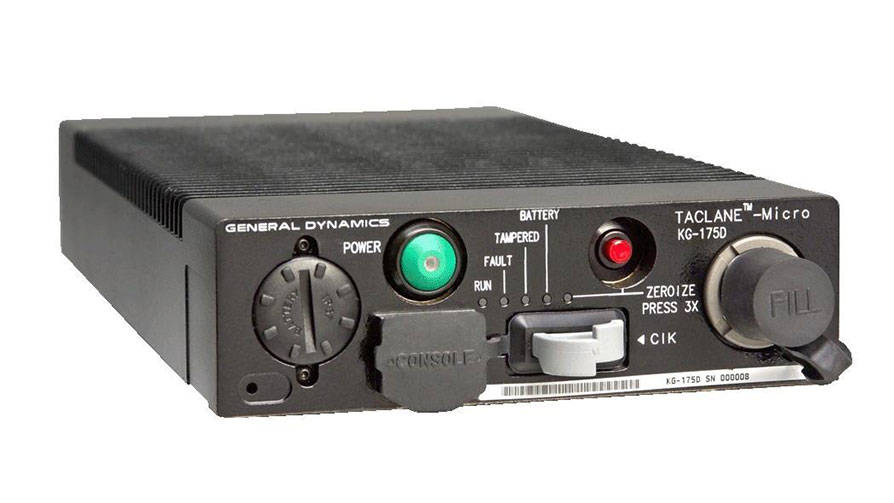
\includegraphics[scale=0.3]{paper/images/taclane.jpg}
\end{center}
\end{frame}

\begin{frame}[fragile]{...why?}
\begin{itemize}
    \item  Modern, hardware-based encryption exist
    \vspace{1em}
        \item Lessons from history
        \begin{itemize}
            \item Breaking down encryption schemes into smaller components
            \item Operator error and key distribution security 
            \item International cooperation in cryptography
        \end{itemize}
\end{itemize}
\end{frame}


\begin{frame}[fragile]{...why?}
\begin{center}
    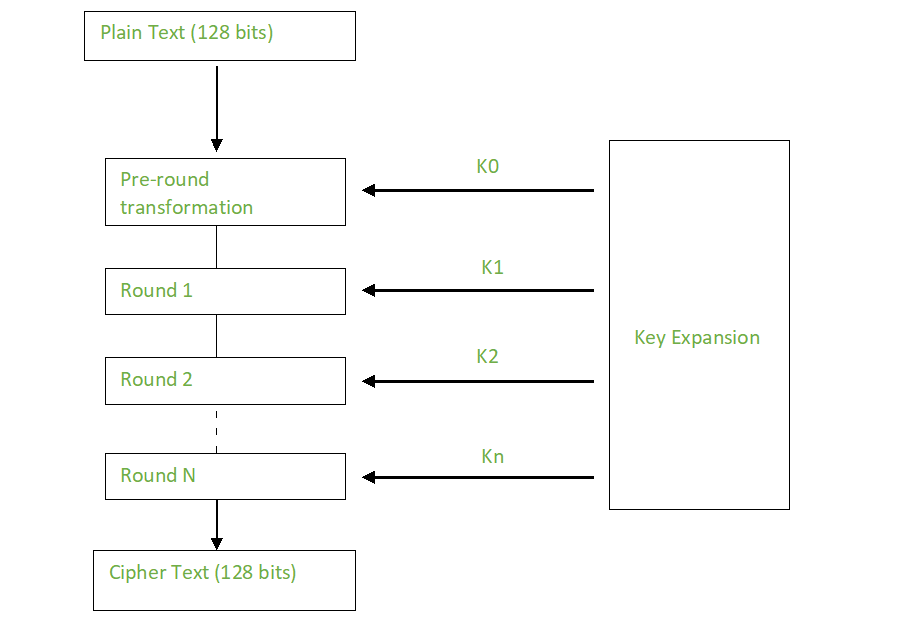
\includegraphics[scale=0.3]{paper/images/aes.png}
\end{center}
\end{frame}

\begin{frame}[fragile]{...why?}
\begin{itemize}
    \item  Modern, hardware-based encryption exist
    \vspace{1em}
        \item Lessons from history
        \begin{itemize}
            \item Breaking down encryption schemes into smaller components
            \item Operator error and key distribution security 
            \item International cooperation in cryptography
        \end{itemize}
    \vspace{1em}
        \item New discoveries by examining ``outdated'' subjects
    \vspace{1em}
    \pause
    \item How did modern computing come to exist?
        \vspace{1em}
    \pause
    \item Specialty built analog computers
\end{itemize}
\end{frame}

\begin{frame}[fragile]{How does Turing's model work?}
Using Dixon's Theorem, we calculate for two loops (not accurate but fine for a heuristic argument)
\begin{itemize}
    \item $95.9\%$ -- $26^1$
    \item  $4.1\%$ -- non-$26^1$ (i.e.\ stops)
    \begin{itemize}
        \item $92.3\%$ -- $1^125^1$
    \end{itemize}
\end{itemize}
\end{frame}

\begin{frame}[fragile]{How does Turing's model work?}
If all stops were $1^125^1$ stops then
\begin{enumerate}
  \item All stops have a steckering hypothesis producing a normal stop.
  \item The number of steckering hypothesis producing a normal stop
    for each stop type is $1$.
\end{enumerate}
so Turing's estimate becomes the true number of stops.
\end{frame}

\begin{frame}[fragile]{How does Turing's model work?}
As a heuristic consider the Orbit-Stabilizer Theorem 
\begin{theorem}[Orbit-Stabilizer Theorem]
  For a group $G$ acting on a finite set $X$, we have that for $x\in X$
  \begin{align*}
    |G\cdot x| = \frac{|G|}{|G_x|}
  \end{align*}
  where $G\cdot x$ is the orbit of $x$ and $G_x$ is the stabilizer of $x$.
\end{theorem}
\end{frame}


\begin{frame}[fragile]{Generalized Dixon's Theorem Sanity Check}
\begin{theorem}
  For $\sigma,\tau\in S_n$ with cycle types, $\alpha$ and $\beta$
  respectively, we have
  \begin{align*}
    &t_{\alpha, \beta}\ = 
    \\&1 -
    \frac{Z(\alpha)Z(\beta)}{(n!)^2}\sum_{(\upsilon_1,\dots,\upsilon_k)\ne(n)}\frac{n!}{Y(m^{(\upsilon)})}\sum_{\alpha^{(\upsilon_j)}\in
    S_{\alpha,\upsilon}}\sum_{\beta^{(\upsilon_j)}\in
    S_{\beta,\upsilon}}\prod_{j=1}^k
    {\frac{(\upsilon_j!)^2}{Z(\alpha^{(\upsilon_j)})Z(\beta^{(\upsilon_j)})}}\cdot
    t_{\alpha^{(\upsilon_j)},\beta^{(\upsilon_j)}}.
  \end{align*}
\end{theorem}
\end{frame}

\begin{frame}[fragile]{Generalized Dixon's Theorem Sanity Check}
\begin{center}
\[
  t_n = \sum_{\alpha,\beta}\frac{1}{Z(\alpha)Z(\beta)}\cdot t_{\alpha,\beta}
\]
\end{center}
\end{frame}

\begin{frame}[fragile]{Finding Plaintext-Ciphertext Pairings}
\begin{center}
\begin{align*}
  & \texttt{QFZWRWIVTYRESXBFOGKUHQBAISEZ}
  \\
  & \texttt{WETTERVORHER}{\uline{\texttt{S}}}\texttt{AGEBISKAYA.....}
  \\
  &
  \texttt{.WETTER}{\uline{\texttt{V}}}\texttt{ORH}{\uline{\texttt{E}}}\texttt{RSAGEBISKAY}{\uline{\texttt{A}}}\texttt{....}
  \\
  & \texttt{..WETTE}{\uline{\texttt{R}}}\texttt{VORHERSAGEBISKAYA...}
  \\
  &
  \texttt{...}{\uline{\texttt{W}}}\texttt{ETTERVORHERSA}{\uline{\texttt{G}}}\texttt{EBISK}{\uline{\texttt{A}}}\texttt{YA...}
  \\
  & \texttt{....WETTERVORHERSAGEBISKAYA..}
  \\
\end{align*}
\end{center}
\end{frame}

\begin{frame}[fragile]{Finding Plaintext-Ciphertext Pairings}
\begin{center}
\begin{figure}[H]
  \begin{center}
    \scalebox{0.5}{
      \begin{tikzpicture}[>=stealth, every node/.style={}]
        % Manual node positions
        \node (E) at (0,0) {\texttt{E}};
        \node (O) at (3,1.5) {\texttt{0}};
        \node (B) at (0,3) {\texttt{B}};
        \node (U) at (-3,3) {\texttt{U}};
        \node (S) at (6,3) {\texttt{S}};
        \node (Y) at (9,3) {\texttt{Y}};
        \node (G) at (-6,3) {\texttt{G}};
        \node (H) at (0,6) {\texttt{H}};
        \node (X) at (-3,6) {\texttt{X}};
        \node (W) at (3,0) {\texttt{W}};
        \node (R) at (6,0) {\texttt{R}};
        \node (F) at (9,0) {\texttt{F}};
        \node (A) at (-3,0) {\texttt{A}};
        \node (I) at (-3,-3) {\texttt{I}};
        \node (Q) at (-6,-3) {\texttt{Q}};
        \node (T) at (0,-3) {\texttt{T}};
        \node (K) at (-6,0) {\texttt{K}};
        \node (V) at (6,-3) {\texttt{V}};

        % Connections
        \draw[-] (E) -- (W) node[midway, above, sloped] {\texttt{ZZB}};
        \draw[-] (W) -- (R) node[midway, above, sloped] {\texttt{ZZA}};
        \draw[-] (R) -- (F) node[midway, above, sloped] {\texttt{ZZL}};
        \draw[-] (R) -- (Y) node[midway, above, sloped] {\texttt{ZZF}};
        \draw[-] (E) -- (O) node[midway, above, sloped] {\texttt{ZZH}};
        \draw[-] (O) -- (S) node[midway, above, sloped] {\texttt{ZZM}};
        \draw[-] (S) -- (Y) node[midway, above, sloped] {\texttt{ZZV}};
        \draw[-] (R) -- (S) node[midway, above, sloped] {\texttt{ZZI}};
        \draw[-] (B) -- (S) node[midway, above, sloped] {\texttt{ZZS}};
        \draw[-] (E) -- (B) node[midway, above, sloped] {\texttt{ZZK}};
        \draw[-] (B) -- (H) node[midway, above, sloped] {\texttt{ZZQ}};
        \draw[-] (X) -- (H) node[midway, above, sloped] {\texttt{ZZJ}};
        \draw[-] (U) -- (E) node[midway, above, sloped] {\texttt{ZZP}};
        \draw[-] (G) -- (A) node[midway, above, sloped] {\texttt{ZZN}};
        \draw[-] (A) -- (E) node[midway, above, sloped] {\texttt{ZZW}};
        \draw[-] (K) -- (G) node[midway, above, sloped] {\texttt{ZZO}};
        \draw[-] (K) -- (A) node[midway, above, sloped] {\texttt{ZZT}};
        \draw[-] (T) -- (E) node[midway, above, sloped] {\texttt{ZZE}};
        \draw[-] (I) -- (A) node[midway, above, sloped] {\texttt{ZZU}};
        \draw[-] (Q) -- (I) node[midway, above, sloped] {\texttt{ZZR}};
        \draw[-] (I) -- (T) node[midway, above, sloped] {\texttt{ZZC}};
        \draw[-] (T) -- (V) node[midway, above, sloped] {\texttt{ZZD}};
        \draw[-] (V) -- (R) node[midway, above, sloped] {\texttt{ZZG}};

    \end{tikzpicture}}
  \end{center}
  \caption{Example menu}
  \label{fig:menu}
\end{figure}
\end{center}
\end{frame}

\begin{frame}[fragile]{Diagonal Board}
\begin{figure}[H]
  \begin{center}
    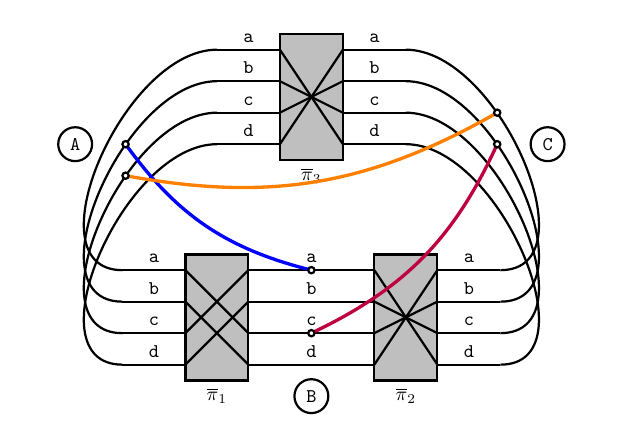
\begin{tikzpicture}[thick, scale=0.4, every node/.style={scale=0.7}]
      % Draw the box
      \draw[fill=lightgray] (2,-1.5) rectangle (4,2.5) node[midway] {};

      \node at (3, -2) {$\overline\pi_3$};

      % Draw the wires entering the box
      \draw[-] (0, 2) -- (2, 2) node[midway, above] {\texttt{a}};
      \draw[-] (0, 1) -- (2, 1) node[midway, above] {\texttt{b}};
      \draw[-] (0, 0) -- (2, 0) node[midway, above] {\texttt{c}};
      \draw[-] (0,-1) -- (2,-1) node[midway, above] {\texttt{d}};

      % Draw the wires exiting the box with crossed mappings
      \draw[-] (4, 2) -- (6,2) node[midway, above] {\texttt{a}};
      \draw[-] (4, 1) -- (6, 1) node[midway, above] {\texttt{b}};
      \draw[-] (4, 0) -- (6, 0) node[midway, above] {\texttt{c}};
      \draw[-] (4,-1) -- (6, -1) node[midway, above] {\texttt{d}};

      % Draw the lines inside the box to represent the mapping
      \draw[-] (2, 2) -- (4, -1);
      \draw[-] (2, 1) -- (4, 0);
      \draw[-] (2, 0) -- (4, 1);
      \draw[-] (2,-1) -- (4, 2);

      \draw[-] (0-3, 2-7) to[out=180, in=180] (0, 2) node[midway, above] {};
      \draw[-] (0-3, 1-7) to[out=180, in=180] (0, 1) node[midway, above] {};
      \draw[-] (0-3, 0-7) to[out=180, in=180] (0, 0) node[midway, above] {};
      \draw[-] (0-3, -1-7) to[out=180, in=180] (0, -1)
      node[midway, above] {};

      \draw[-] (6+3, 2-7) to[out=360, in=360] (6, 2) node[midway, above] {};
      \draw[-] (6+3, 1-7) to[out=360, in=360] (6, 1) node[midway, above] {};
      \draw[-] (6+3, 0-7) to[out=360, in=360] (6, 0) node[midway, above] {};
      \draw[-] (6+3, -1-7) to[out=360, in=360] (6, -1) node[midway, above] {};

      \draw[fill=lightgray] (2-3,-1.5-7) rectangle (4-3,2.5-7) node[midway] {};

      \node at (3-3, -2-7) {$\overline\pi_1$};

      % Draw the wires entering the box
      \draw[-] (0-3, 2-7) -- (2-3, 2-7) node[midway, above] {\texttt{a}};
      \draw[-] (0-3, 1-7) -- (2-3, 1-7) node[midway, above] {\texttt{b}};
      \draw[-] (0-3, 0-7) -- (2-3, 0-7) node[midway, above] {\texttt{c}};
      \draw[-] (0-3,-1-7) -- (2-3,-1-7) node[midway, above] {\texttt{d}};

      % Draw the wires exiting the box
      \draw[-] (4-3, 2-7) -- (6-3,2-7) node[right, above] {\texttt{a}};
      \draw[-] (4-3, 1-7) -- (6-3, 1-7) node[right, above] {\texttt{b}};
      \draw[-] (4-3, 0-7) -- (6-3, 0-7) node[right, above] {\texttt{c}};
      \draw[-] (4-3,-1-7) -- (6-3, -1-7) node[right, above] {\texttt{d}};

      % Draw the lines inside the box to represent the mapping
      \draw[-] (2-3, 2-7) -- (4-3, 0-7);
      \draw[-] (2-3, 1-7) -- (4-3, -1-7);
      \draw[-] (2-3, 0-7) -- (4-3, 2-7);
      \draw[-] (2-3,-1-7) -- (4-3, 1-7);

      \draw[fill=lightgray] (2+3,-1.5-7) rectangle (4+3,2.5-7) node[midway] {};

      \node at (3+3, -2-7) {$\overline\pi_2$};

      % Draw the wires entering the box
      \draw[-] (0+3, 2-7) -- (2+3, 2-7) node[midway, above] {};
      \draw[-] (0+3, 1-7) -- (2+3, 1-7) node[midway, above] {};
      \draw[-] (0+3, 0-7) -- (2+3, 0-7) node[midway, above] {};
      \draw[-] (0+3,-1-7) -- (2+3,-1-7) node[midway, above] {};

      % Draw the wires exiting the box
      \draw[-] (4+3, 2-7) -- (6+3,2-7) node[midway, above] {\texttt{a}};
      \draw[-] (4+3, 1-7) -- (6+3, 1-7) node[midway, above] {\texttt{b}};
      \draw[-] (4+3, 0-7) -- (6+3, 0-7) node[midway, above] {\texttt{c}};
      \draw[-] (4+3,-1-7) -- (6+3, -1-7) node[midway, above] {\texttt{d}};

      \draw[-] (2+3, 2-7) -- (4+3, -1-7);
      \draw[-] (2+3, 1-7) -- (4+3, 0-7);
      \draw[-] (2+3, 0-7) -- (4+3, 1-7);
      \draw[-] (2+3,-1-7) -- (4+3, 2-7);

      \node[draw,circle] at (-4.5, -1) {\texttt{A}};
      \node[draw,circle] at (3, -9) {\texttt{B}};
      \node[draw,circle] at (10.5, -1) {\texttt{C}};

      % Diagonal wires
      \draw[-, blue, very thick] (3,2-7) to[bend left=20] (-3+0.1, 2-3);
      \draw[fill=white] (-3+0.1, 2-3) circle (0.1);
      \draw[fill=white] (3, 2-7) circle (0.1);

      \draw[-, orange,  very thick] (9-0.1,2-2) to[bend left=20] (-3+0.1, 2-4);
      \draw[fill=white] (9-0.1, 2-2) circle (0.1);
      \draw[fill=white] (-3+0.1, 2-4) circle (0.1);

      \draw[-, purple, very thick] (3,0-7) to[bend right=20] (9-0.1, 2-3);
      \draw[fill=white] (3, 0-7) circle (0.1);
      \draw[fill=white] (9-0.1, 2-3) circle (0.1);

    \end{tikzpicture}
  \end{center}
  \caption{Diagonal wires}
  \label{fig:diagonal}
\end{figure}
\end{frame}

\end{document}
